%%%%%%%%%%%%%%%%%%%%%%%%%%%%%%%%%%%%%%%%%%%%%%%%%%
% 载入模版
%
% 载入csuthesis.cls文件定义的模板
% 支持选项,forprint(黑白打印模式)
% 载入主体内容样式与参考文献样式
%%%%%%%%%%%%%%%%%%%%%%%%%%%%%%%%%%%%%%%%%%%%%%%%%%
% 选项
%   type=[bachelor|research|translation],                  % 可选(默认:bachelor),论文类型(学位or课程/调研报告/文献翻译)
%   output=[print|electronic],                            % 可选(默认:print),输出要求(电子版/打印)
\documentclass[type=bachelor, output=electronic, fontset=none]{csuthesis}
% 来自https://github.com/hushidong/biblatex-gb7714-2015
% 参考文献 gb7714-2015 支持宏包
% 使用了biblatex-gb7714-2015宏包,指定后端为biber
\usepackage[backend=biber,style=gb7714-2015,gbnamefmt=lowercase,gbpub=false,gbpunctin=false, doi=false, url=false]{biblatex}
% 重定义参考文献字体为楷体GB_2312 字号5号
\renewcommand{\bibfont}{\zihao{5} \kgb}
% 导入参考文献数据库
\addbibresource{csuthesis_main.bib}
% 按照章节(chapter)标注图片和表格序号,亦可根据需要改为section等
\counterwithin{figure}{chapter}
\counterwithin{table}{chapter}

% 公式、图片、表格序号改成(1-1)的形式
\renewcommand{\theequation}{\thechapter-\arabic{equation}}
\renewcommand\thefigure{\arabic{chapter}-\arabic{figure}}
\renewcommand\thetable{\arabic{chapter}-\arabic{table}}

\usepackage{array}
\newcolumntype{L}[1]{>{\raggedright\let\newline\\\arraybackslash\hspace{0pt}}m{#1}}
\newcolumntype{C}[1]{>{\centering\let\newline\\\arraybackslash\hspace{0pt}}m{#1}}
\newcolumntype{R}[1]{>{\raggedleft\let\newline\\\arraybackslash\hspace{0pt}}m{#1}}

% 各级小标题前后间距:前后各一个字符,首行缩进俩字符
% \titlespacing{\section}{0pt}{2.5ex plus 1ex minus .2ex}{1.3ex plus .2ex}
% \titlespacing{\section}{2em}{*0.5}{*0.5}
% \titlespacing{\subsection}{2em}{*0}{*0}

% 设置有序列表和无序列表缩进
\setlist[enumerate]{leftmargin=4em}
% \setlist[itemize]{leftmargin=4em}

% 将伪代码的require和ensure修改为input和output
\renewcommand{\algorithmicrequire}{\textbf{Input:}}
\renewcommand{\algorithmicensure}{\textbf{Output:}}


%%%%%%%%%%%%%%%%%%%%%%%%%%%%%%%%%%%%%%%%%%%%%%%%%%
% 基本信息
%
% 用户自行输入标题、作者等基本信息
% 都存储在\content\info.tex文件中
%%%%%%%%%%%%%%%%%%%%%%%%%%%%%%%%%%%%%%%%%%%%%%%%%%
%!TEX root = ../csuthesis_main.tex
% 文章信息
\titlecn{考虑边缘计算的无人机航迹规划及任务调度研究}
\titleen{Research on trajectory planning and mission scheduling of UAV considering edge computing}

\priormajor{}     % 主修
\minormajor{}       % 辅修(选填)
\interestmajor{}  % 兴趣(选填)
\author{}              % 作者
\supervisor{}        % 指导老师
\subsupervisor{}
\department{}         % 学院
\studentid{}          % 学号
\thesisdate{year=2022,month=5}  % 时间
\myclass{}        % 班级


%以下的对本科生没有用
\clcnumber{TP391} 				% 中图分类号 Chinese Library Classification
\schoolcode{10533}			% 学校代码
\udc{004.9}						% UDC
\academiccategory{学术学位}	% 学术类别



\begin{document}
%%%%%%%%%%%%%%%%%%%%%%%%%%%%%%%%%%%%%%%%%%%%%%%%%%
% 封面绘制
%
% 1.5版本重新编写了封面绘制宏,并用latex使用者更习惯的
% \maketitle代替之前的\makecoverpage
%%%%%%%%%%%%%%%%%%%%%%%%%%%%%%%%%%%%%%%%%%%%%%%%%%
\maketitle

% 启用大罗马字母进行编号
\frontmatter
% 设置页眉和页脚


%%%%%%%%%%%%%%%%%%%%%%%%%%%%%%%%%%%%%%%%%%%%%%%%%%
% 中文摘要
%
% 存储在\content\abstractzh.tex文件中
%%%%%%%%%%%%%%%%%%%%%%%%%%%%%%%%%%%%%%%%%%%%%%%%%%
%!TEX root = ../csuthesis_main.tex
% 设置中文摘要
\keywordscn{多无人机\quad 边缘计算\quad 任务分配\quad 航迹规划\quad 资源调度\quad 智能优化算法}
%\categorycn{TP391}
\begin{abstractzh}

近年来,随着无人机技术的不断发展,无人机在军事和民用领域都得到了广泛的应用。为了推广无人机在城市环境下的应用,本文针对无人机航迹规划及任务调度问题进行研究,在对该问题进行详细描述及分析的基础上,基于边缘计算架构将其分解为了任务计算资源调度问题、多无人机航迹规划及任务分配问题共两个子问题,分别建立了相应的数学模型,并通过设计基于ASA算法的静态任务计算资源调度算法、基于FD算法的动态任务计算资源调度算法、基于RRT*-Connect算法的静态场景下的无人机航迹规划算法、基于A*算法的动态场景下的无人机航迹规划算法以及基于TSAVN算法的多无人机任务分配算法实现对上述两个子问题的求解。最后,对于各个子问题分别设计了相应的仿真实验,验证了本文所提出的算法在求解考虑边缘计算的无人机航迹规划及任务调度各个子问题的有效性及优越性。

仿真实验结果表明:
% 任务计算资源调度问题
在任务计算资源调度问题中,ASA算法能够在考虑传输时延等情况下生成较优的计算资源调度方案,同时相较于其他对比算法,其生成的计算资源调度方案与算法的运行时间都有着显著的优越性和鲁棒性;而FD算法相较于其他对比算法,虽然其生成的计算资源调度方案较差,但其运行时间能够满足问题场景下所需要的实时性。
% 多无人机航迹规划及任务分配问题
在多无人机航迹规划及任务分配问题中,RRT*-Connect算法的能够在城市密集障碍物静态场景下快速规划出优良的无人机飞行航迹,相较于其他对比算法,其规划的飞行航迹有着更好的性能和鲁棒性;A*算法能够根据实时获取的障碍物信息对无人机飞行航迹进行快速修订,相较于其他对比算法,其生成的飞行航迹与运行时间都有着显著的优越性和鲁棒性;同时的TSAVN算法能够根据所给飞行航程信息与任务信息,在较短时间内生成无人机的收集型侦察任务分配方案,相较于其他对比算法,其生成的任务分配方案以及算法的运行时间都有着显著的优越性与鲁棒性。

\end{abstractzh}


%%%%%%%%%%%%%%%%%%%%%%%%%%%%%%%%%%%%%%%%%%%%%%%%%%
% 英文摘要
%
% 存储在\content\abstracten.tex文件中
%%%%%%%%%%%%%%%%%%%%%%%%%%%%%%%%%%%%%%%%%%%%%%%%%%
%!TEX root = ../csuthesis_main.tex
\keywordsen{Multi-UAV\ \ Edge Computing\ \ Task Scheduling\ \ Trajectory Planning\ \ Resource Scheduling\ \ Intelligent Optimization Algorithm}
\begin{abstracten}

In recent years, with the continuous development of UAV technology, UAVs have been widely used in both military and civilian fields. In order to promote the application of UAVs in urban environments, this thesis investigates the UAV task scheduling and dynamic trajectory planning problem. Based on a detailed description and analysis of the problem, it is decomposed into two sub-problems based on edge computing architecture: the task computing resource scheduling problem, the multi-UAV task allocation and trajectory planning problem, and the single-UAV real-time obstacle avoidance problem. The corresponding mathematical models are established, and the above sub-problems are solved by designing the static mission computing resource scheduling algorithm based on ASA algorithm, the dynamic mission computing resource scheduling algorithm based on FD algorithm, the UAV trajectory planning algorithm in static scenes based on RRT*-Connect algorithm, the UAV trajectory planning algorithm in dynamic scenes based on A* algorithm and the multi-UAV mission allocation algorithm based on TSAVN algorithm algorithm based on A* algorithm. Finally, the corresponding simulation experiments are designed for each subproblem to verify the effectiveness and superiority of the proposed algorithms in solving each subproblem of UAV task scheduling and dynamic trajectory planning considering edge computing.

The simulation experimental results show that 
% 任务计算资源调度问题
in the task computational resource scheduling problem, the ASA algorithm is able to generate a better computational resource scheduling scheme resource information, considering the transmission delay. At the same time, its generated computational resource scheduling scheme and the running time of the algorithm are significantly superior and robust compared to other comparative algorithms. The FD algorithm, on the other hand, generates a poorer computational resource scheduling scheme compared to other comparative algorithms, but its running time can meet the real-time performance required in the problem scenario.
% 多无人机航迹规划及任务分配问题
In the multi-UAV mission assignment and trajectory planning problem, the RRT*-Connect algorithm is able to quickly plan excellent UAV flight trajectories in urban dense obstacle scenarios with better performance and robustness compared to other comparative algorithms; the A* algorithm can quickly revise the UAV flight trajectory based on the obstacle information acquired in real time, which has significant superiority and robustness in terms of generated flight trajectory and running time compared to other comparative algorithms;meanwhile, the TSAVN algorithm is able to generate UAV collection-based reconnaissance mission assignment schemes in a short time based on the given flight distance information and mission information, which has significant superiority and robustness compared to other comparative algorithms in terms of the generated mission assignment schemes and the running time of the algorithm.

\end{abstracten}



%%%%%%%%%%%%%%%%%%%%%%%%%%%%%%%%%%%%%%%%%%%%%%%%%%
% 目录
%
% 使用重定义的tableofcontents宏绘制目录
% 满足学校的样式要求
%%%%%%%%%%%%%%%%%%%%%%%%%%%%%%%%%%%%%%%%%%%%%%%%%%
\tableofcontents


% 启用数字编号,改为第 x 页  共 x 页格式
\mainmatter

%%%%%%%%%%%%%%%%%%%%%%%%%%%%%%%%%%%%%%%%%%%%%%%%%%
% 正文
%
% 存储在\content\content.tex文件中
%%%%%%%%%%%%%%%%%%%%%%%%%%%%%%%%%%%%%%%%%%%%%%%%%%
% 正文
%!TEX root = ../csuthesis_main.tex

%子章节为了便于查找和修改,建议通过input拆分文件

%!TEX root = ../../csuthesis_main.tex
\chapter{绪论}


\section{研究背景及意义}

5G (5th-Generation) 通信技术,即第五代移动通信技术,为4G通信技术的进一步发展的新技术。由于5G通信技术与此前的4G通信技术相比,有着高速率、宽带宽、高可靠、低时延等优势,能够满足在自动驾驶、远程医疗等方面的应用的要求,同时在如今新基建的浪潮下,5G技术与AI、物联网等技术应用得以如雨后春笋般迅猛发展,带来了信息流量及运算算力等方面的巨大变化。

如图~\ref{fig:2016-2021年移动互联网流量及月户均流量(DOU)增长情况}所示,根据\href{https://www.miit.gov.cn/gxsj/tjfx/txy/art/2022/art_e8b64ba8f29d4ce18a1003c4f4d88234.html}{2021年通信业统计公报}的数据,截止2021年底,移动互联网产生的流量比上年增长33.9\%,共达2216亿GB,其中手机上网流量就已达到2125亿GB,在总流量中占比高达95.9\%;与此同时物联网用户已达13.99亿户,比上年增长23.3\%,其中应用于智慧公共视野、智能制造、智慧交通的终端用户占比分别达22.4\%、18.1\%、15.6\%。从以上数据可知,数据流量和物联网还在如喷涌般迅速发展,使得数据的分析和处理也有着极大且还在快速增长的需求。

\begin{figure}[!htbp]
    \centering
    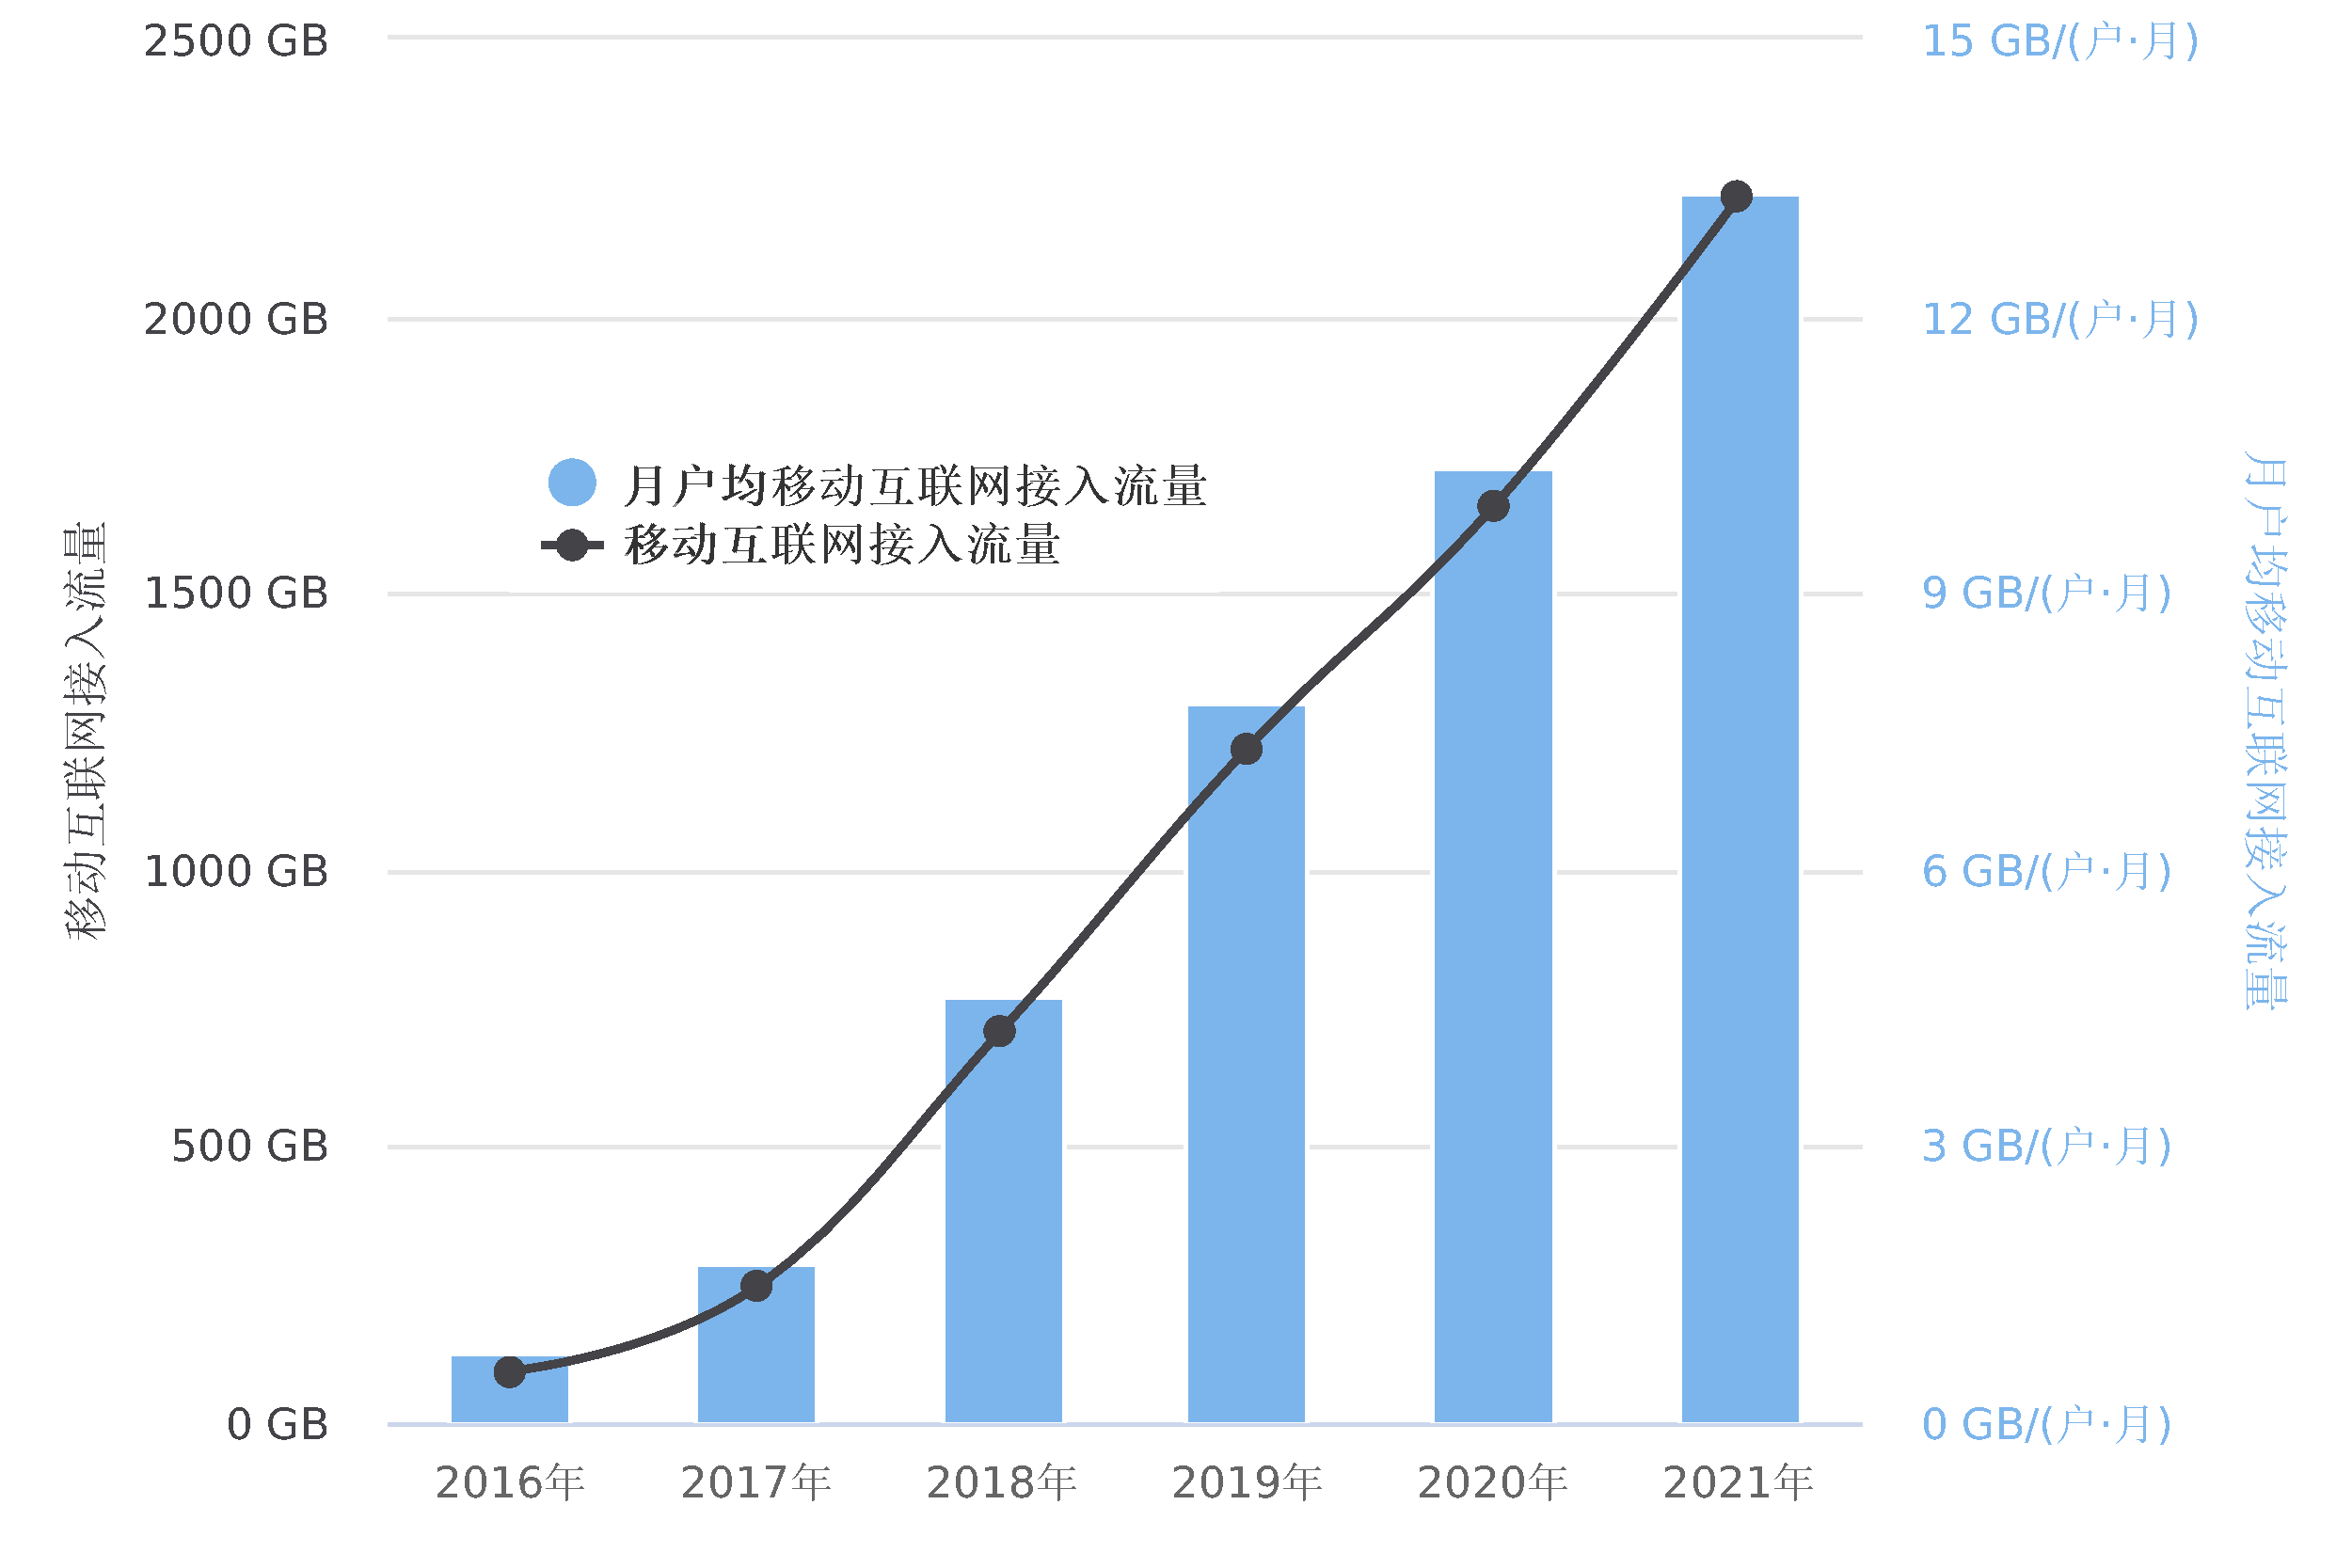
\includegraphics[width=0.75\textwidth]{./images/2016-2021年移动互联网流量及月户均流量(DOU)增长情况.pdf}
    \caption{2016-2021年移动互联网流量及月户均流量(DOU)增长情况(来源:\href{https://www.miit.gov.cn/gxsj/tjfx/txy/art/2022/art_e8b64ba8f29d4ce18a1003c4f4d88234.html}{2021年通信业统计公报})}
    \label{fig:2016-2021年移动互联网流量及月户均流量(DOU)增长情况}
\end{figure}

5G通信技术及其他技术的迅猛发展,促使了用户的边缘数据量快速增长。随着边缘数据量不断增大,在数据传输时存在通信占用带宽过多、处理时占用负载较大、储存占用空间过多、边缘设备性能使用率较低等问题。为了解决这些问题,研究学者提出了将一部分任务分配至边缘设备中进行处理的边缘计算技术,能够应用于在靠近用户或数据源的边缘设备中,为其提供网络、计算、储存等所需服务。通过这一技术降低了数据中心服务器的荷载,并且为用户提供了高稳定和低时延的良好使用体验;延伸了数据中心-用户的计算框架并形成了数据中心-边缘设备-用户的新型框架;还有助于数据、算力、成本的灵活布置,有助于对时延、稳定性等性能要求较高的需求的满足。

UAV (Unmanned Aerial Vehicle, 无人机)是一种机上无需载乘任何操作人员、能够自主控制或由机组人员远程遥控的,可搭载一定设备且能够重复利用的无人飞行平台及设备。近些年,无论在科学研究还是在应用市场中,针对UAV的研究和应用受到了越来越广泛的关注,其民用市场规模也逐年递增(见图~\ref{fig:2015-2020年中国民用无人机市场规模})。同时,随着相关技术的快速发展,UAV的自身性能得到了迅速增强,与传统的载人飞行器相比,UAV的性价比更高,且具有体积小、重量轻、灵活性好、机动性强,易部署、成本低、广视角、隐蔽性好等诸多优点。

\begin{figure}[!htbp]
    \centering
    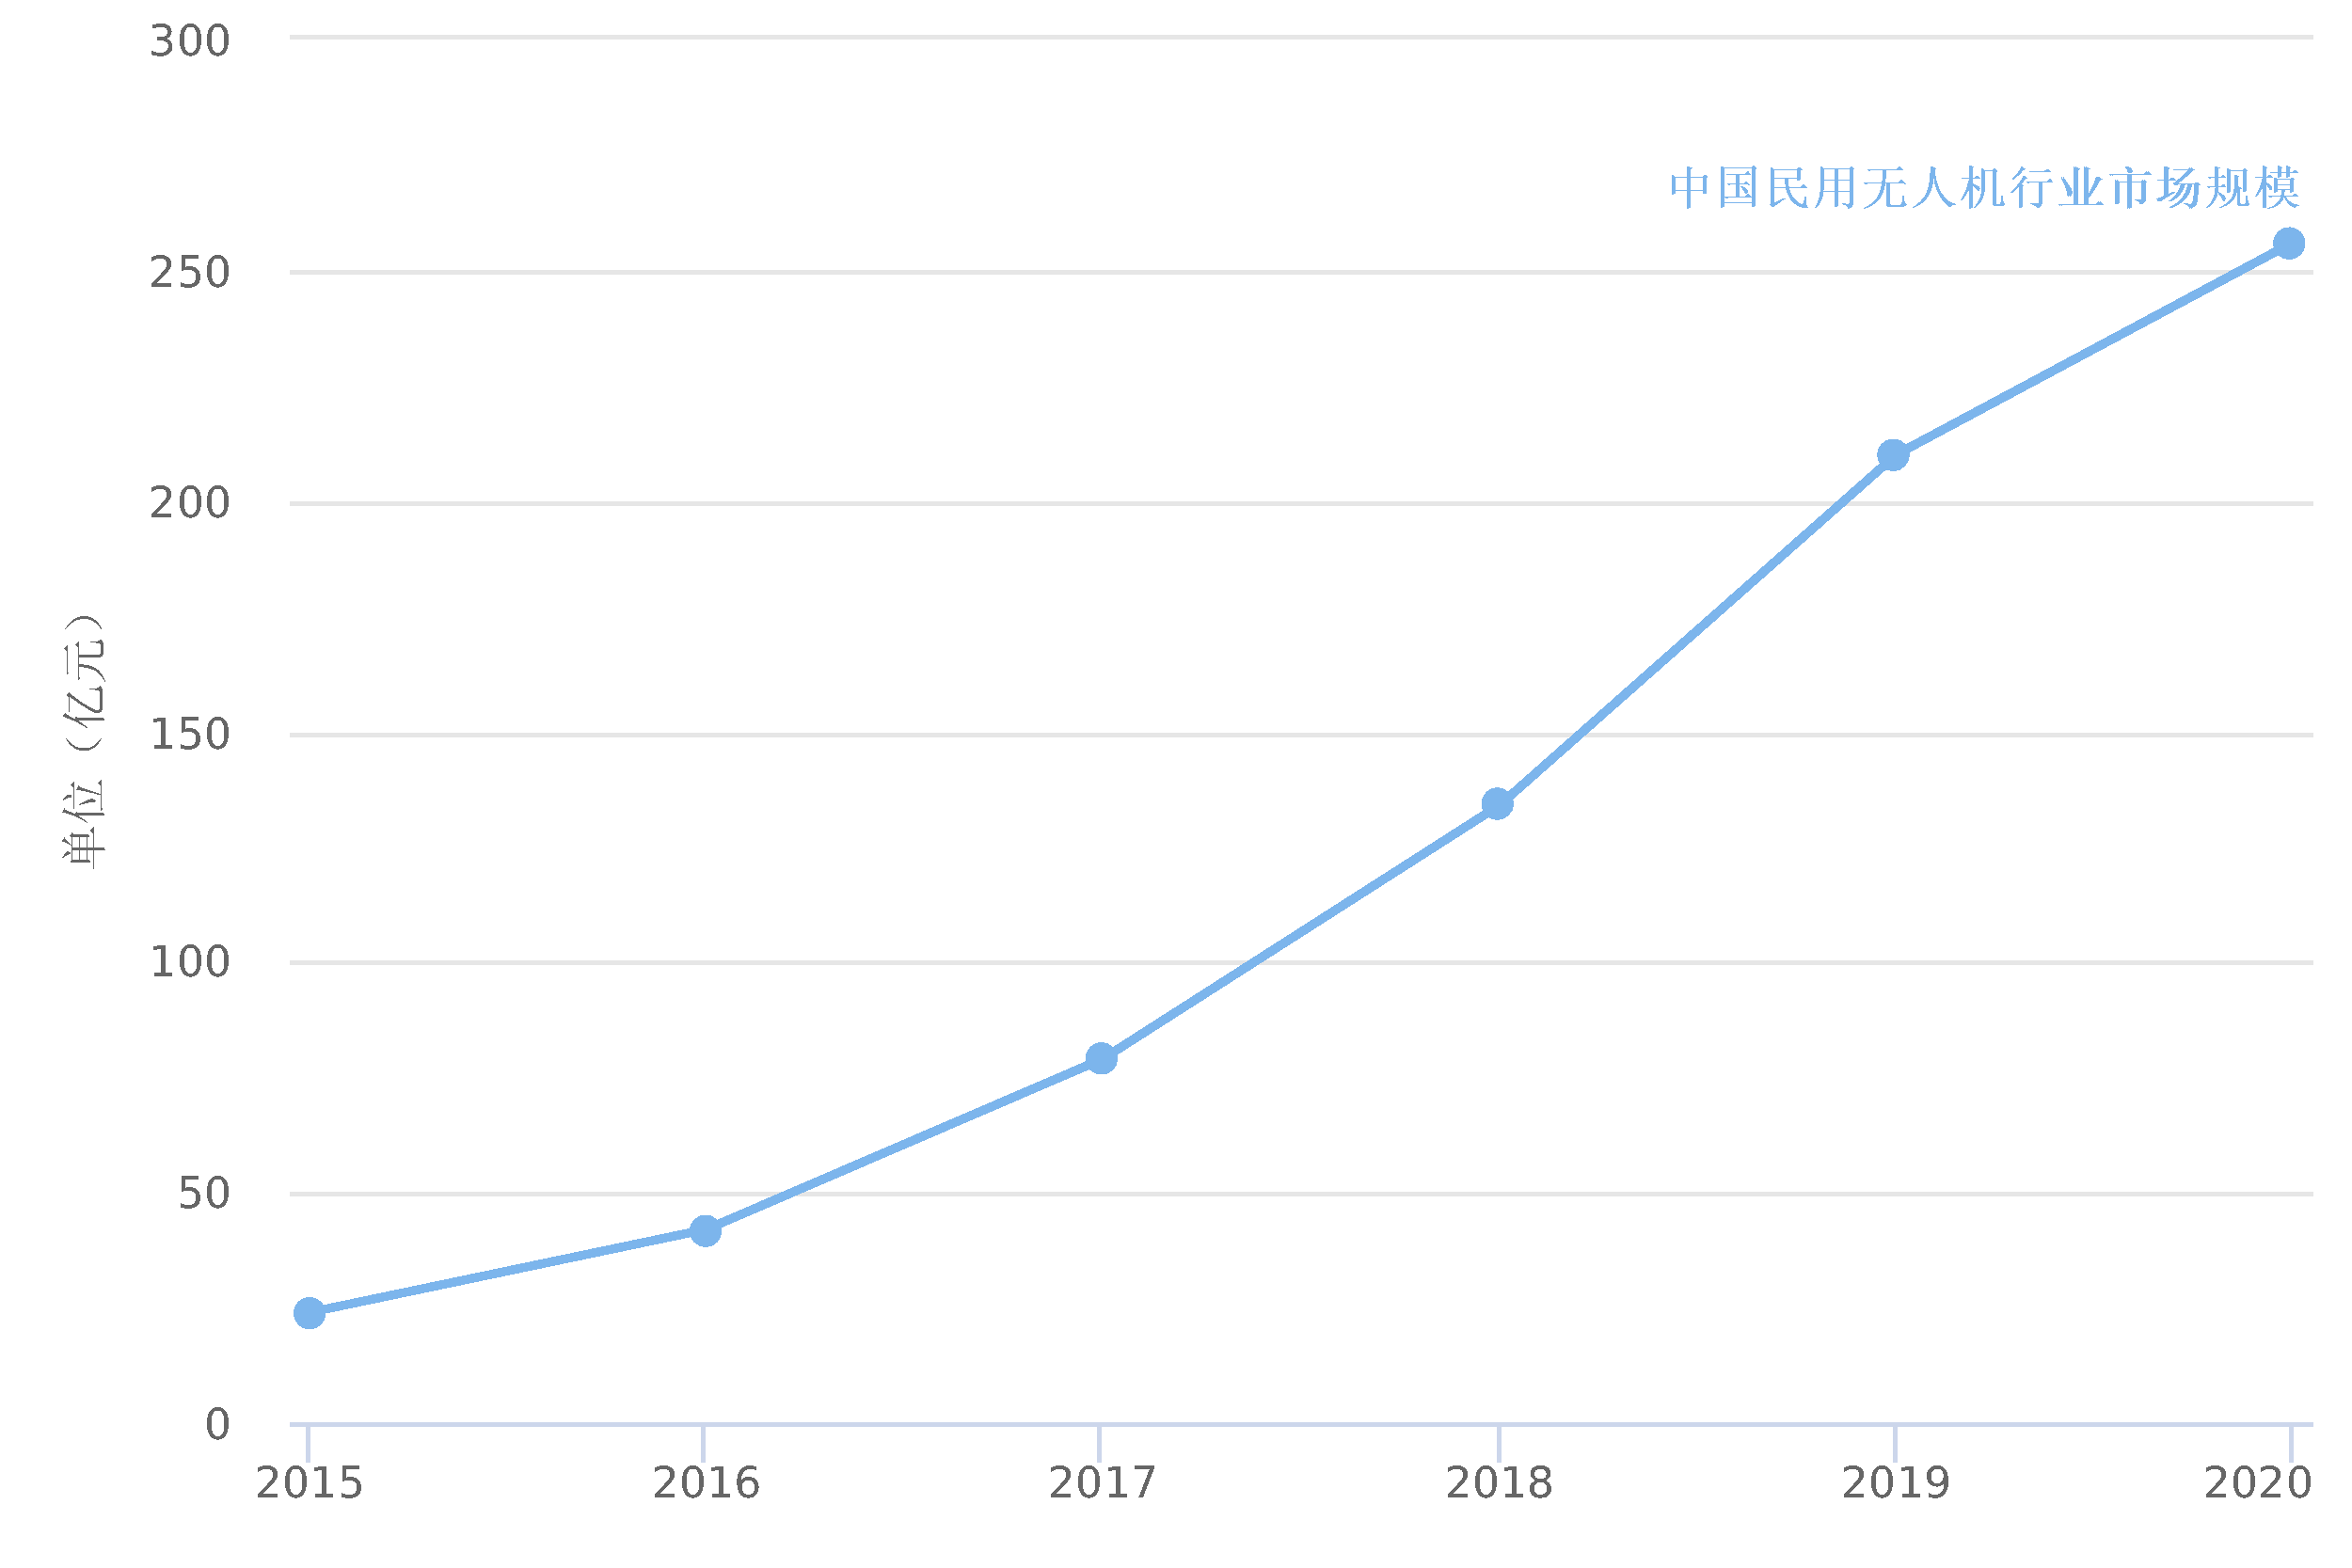
\includegraphics[width=0.75\textwidth]{images/2015-2020年中国民用无人机市场规模.pdf}
    \caption{2015-2020年中国民用无人机市场规模(来源:\href{https://bg.qianzhan.com/trends/detail/506/220215-4753a4d9.html}{前瞻产业研究院})}
    \label{fig:2015-2020年中国民用无人机市场规模}
\end{figure}

UAV的上述优点加速了其在相关民用和军事领域的应用,如图~\ref{fig:集群无人机应用场景}所示,UAV目前常应用于在铁路故障巡检、交通调查、物流配送\citep{peng2019HybridGeneticAlgorithma}、灾难响应\citep{yang2020MaritimeSearchRescuea}、森林火情监视等民用邻域,以及集群作战\citep{liu2018MeiJunZhuYaoWuRenJiJiQunXiangMuFaZhanQianXia}、对地目标打击等军事领域。目前美军出台了多个无人机项目,例如低成本无人机集群技术项目、小精灵项目、进攻性集群使能战术项目等,大力推动发展各类场景下人机协同或集群作战的能力,走在了世界前列\citep{liu2018MeiJunZhuYaoWuRenJiJiQunXiangMuFaZhanQianXia}。但目前无人机也存在着单机计算能力较弱的缺点\citep{yao2013WuRenJiQunXieTongZuoZhanRenWuFenPeiFangFaYanJiu},因此,将边缘计算技术引入无人机应用领域已经成为无人机的发展方向之一。

\begin{figure}[!htbp]
    \centering
    \begin{subfigure}[t]{0.35\textwidth}
        \captionsetup{justification=centering}
        \begin{minipage}[b]{1\linewidth}
            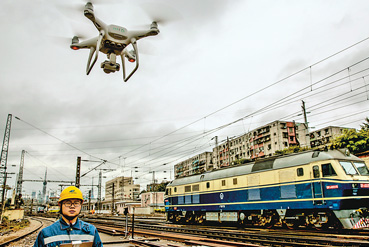
\includegraphics[width=\textwidth]{./images/铁路巡检.png}
            \caption{铁路巡检}
        \end{minipage}
    \end{subfigure}
    \begin{subfigure}[t]{0.3\textwidth}
        \captionsetup{justification=centering}
        \begin{minipage}[b]{1\linewidth}
            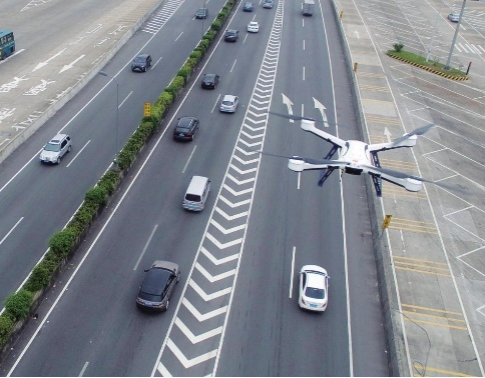
\includegraphics[width=\textwidth]{./images/交通调查.png}
            \caption{交通调查}
        \end{minipage}
    \end{subfigure}
    \begin{subfigure}[t]{0.275\textwidth}
        \captionsetup{justification=centering}
        \begin{minipage}[b]{1\linewidth}
            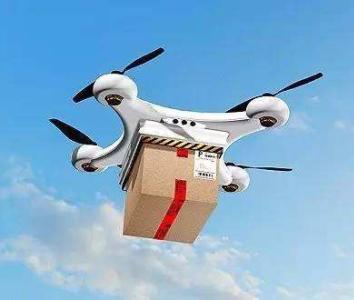
\includegraphics[width=\textwidth]{./images/物流配送.png}
            \caption{物流配送}
        \end{minipage}
    \end{subfigure}

    \begin{subfigure}[t]{0.3\textwidth}
        \captionsetup{justification=centering}
        \begin{minipage}[b]{1\linewidth}
            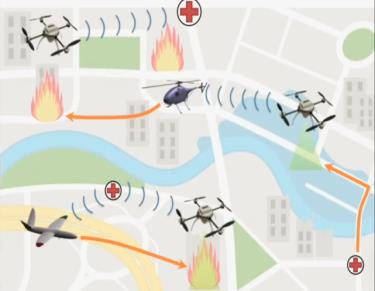
\includegraphics[width=\textwidth]{./images/灾难响应.png}
            \caption{灾难响应}
        \end{minipage}
    \end{subfigure}
    % \hfill
    \begin{subfigure}[t]{0.31\textwidth}
        \captionsetup{justification=centering}
        \begin{minipage}[b]{1\linewidth}
            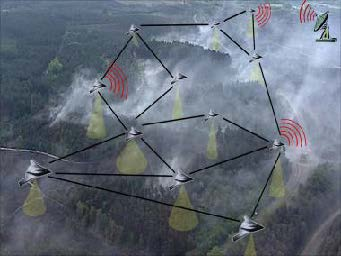
\includegraphics[width=\textwidth]{./images/森林火情监视.png}
            \caption{森林火情监视}
        \end{minipage}
    \end{subfigure}
    % \hfill
    \begin{subfigure}[t]{0.305\textwidth}
        \captionsetup{justification=centering}
        \begin{minipage}[b]{1\linewidth}
            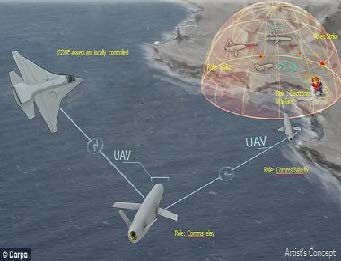
\includegraphics[width=\textwidth]{./images/军事目标打击.png}
            \caption{军事目标打击}
        \end{minipage}
    \end{subfigure}

    \caption{集群无人机应用场景}
    \label{fig:集群无人机应用场景}
\end{figure}

我国“十四五”规划已明确提出要加快将中国建设成为交通强国,UAV作为一种新型的交通运输方式,已经成为“交通强国”战略中的重要一环。将多无人机合理有效地应用于交通领域将有利于促进数字交通体系精细化、信息化,加快智慧交通建设立体化、快速化,以及推动交通运输系统高效化、智能化。作为UAV关键应用之一,面向城市低空环境的多无人机侦察任务,存在着因设备数量多、基站带宽有限等原因而带来的如通信延迟较大、计算性能有限等问题;同时城市低空环境与其他环境相比,有着空间更为狭窄、障碍数量更多且密集,人员活动更为密集等特点,这也对无人机的航迹规划技术在实时性和避障性提出了更高的要求。以上问题使得UAV应用目前还远远达不到“交通强国”战略中的应用需求,而这势必会阻碍我国交通建设迈向更高水平及质量。

基于无人机的边缘计算研究是将边缘计算的架构应用于无人机平台,使得无人机作为边缘端既能够将一定的任务卸载到位于地面基站的服务器中,也可以将一定的任务卸载至其余空闲无人机中的研究,该方法既能够解决数据中心的集中式计算带来的通信占用带宽过多、处理时占用负载较大、储存占用空间过多、边缘设备性能使用率较低等问题,还能够充分利用现有设备的算力,使得设备整体利用率上升,便于控制成本。根据无人机是作为用户节点还是边缘服务器,其可被分为两种不同的场景:一种是无人机作为用户节点,地面基站为其提供计算服务支持,即面向无人机网络的边缘计算场景,如图~\ref{fig:面向无人机网络的边缘计算}所示;另一种是在无人机上装备边缘计算服务器,为地面网络提供计算服务,即面向地面网络的无人机边缘计算场景,如图~\ref{fig:面向地面网络的无人机边缘计算}所示。

\begin{figure}[!htbp]
    \centering
    \begin{subfigure}[t]{0.4\textwidth}
        \captionsetup{justification=centering}
        \begin{minipage}[b]{1\linewidth}
            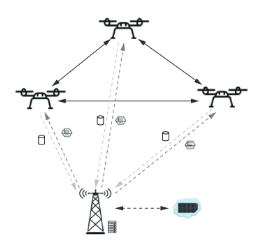
\includegraphics[width=\textwidth]{images/面向无人机网络的边缘计算.png}
            \caption{面向无人机网络的边缘计算}
            \label{fig:面向无人机网络的边缘计算}
        \end{minipage}
    \end{subfigure}
    % \hfill
    \begin{subfigure}[t]{0.55\textwidth}
        \captionsetup{justification=centering}
        \begin{minipage}[b]{1\linewidth}
            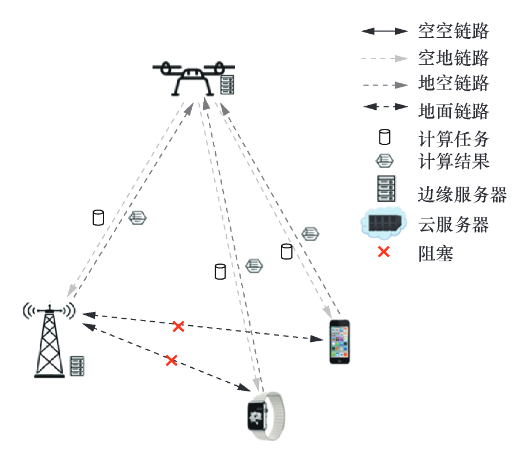
\includegraphics[width=\textwidth]{images/面向地面网络的无人机边缘智能计算.png}
            \caption{面向地面网络的无人机边缘计算}
            \label{fig:面向地面网络的无人机边缘计算}
        \end{minipage}
    \end{subfigure}
    \caption{基于无人机的边缘计算研究场景}
    \label{fig:基于无人机的边缘计算研究场景}
\end{figure}

因此,本文提出面向边缘计算的无人机航迹规划及任务调度方法,以解决在城市低空环境下的多无人机航迹规划及任务调度任务中的局限性,进一步提高系统的性能使用率、降低运算成本,有助于推广UAV在城市低空环境下的可应用性。

\section{国内外研究现状}

\subsection{面向无人机网络的边缘计算研究}

在面向无人机网络的边缘计算研究的场景中,多架无人机联合执行任务,无人机之间通过空空链路进行连接。无人机边缘端将图像分析等计算密集型任务卸载到位于地面基站的地面端服务器上,地面端服务器完成任务处理后将结果返还给无人机,通过这种方式可以大大降低无人机的能耗和任务的处理时延,从而延长无人机的续航时间,并提升任务的完成效率。

在面向无人机网络的边缘计算研究中,通常会采用三种不同的架构,分别是将无人机作为边缘中转设备的用户设备-无人机-地面基站3层架构、\citet{chen2019WhenUAVSwarmb}提出的将无人机作为终端设备的无人机-边缘服务器-云服务器3层架构,以及\citet{cheng2018AirGroundIntegratedMobile}提出的将无人机既作为终端设备也作为边缘设备的空地一体移动边缘架构。到目前为止,面向无人机网络的边缘计算研究在不同架构下所应用的方法主要分为以下三种:博弈论方法、运筹学方法、智能算法,如表~\ref{tab:面向无人机网络的边缘计算研究总结}所示。

\begin{table}[!htbp]
    \caption{面向无人机网络的边缘计算研究总结}
    \label{tab:面向无人机网络的边缘计算研究总结}
    \centering
    \begin{tabular}{c c c}
        \toprule
        \textbf{类型} & \textbf{方法} & \textbf{优缺点} \\
        \midrule
        \multirow{2}{*}{博弈论方法} & 纳什均衡\citep{messous2017ComputationOffloadingGamea} & \multirow{2}{15em}{算法计算快、可靠性强,适用于求解大规模问题场景;容易限于局部最优解,解质量可能较差。} \\
        & 博弈理论 + 纳什均衡\citep{peng2021DuoWuRenJiXieTongZhiBoChangJingXiaZiGuaYingRenWuXieZaiJueCe} & \\
        \cmidrule(lr){1-3}
        \multirow{3}{*}{运筹学方法} & 匈牙利算法\citep{kim2019OptimalTaskUAVEdgeMatchingb} & \multirow{3}{15em}{考虑了无人机位置与延迟的关系,贴近真实场景;实时性强,可用于动态调度;但问题规模较大时计算时间较久。} \\
        & 排队论方法\citep{zhang2020ResponseDelayOptimizationa} & \\
        & 交替优化 + 逐次凸逼近\citep{cao2018MobileEdgeComputinga} & \\
        \cmidrule(lr){1-3}
        \multirow{3}{*}{智能算法} & 模拟退火 + 粒子群算法\citep{zhu2018CooperativeComputationOffloadinga} & \multirow{3}{15em}{算法步骤简单易懂;能在可接受时间内,得出一个较优解;容易限于局部最优解,解质量可能较差。} \\
        & Q-Learning 强化学习算法\citep{kim2020MachineLearningBaseda} & \\
        & 强化学习 + 差分演化算法\citep{yang2020MultiUAVEnabledLoadBalanceMobileEdge} & \\
        \bottomrule
    \end{tabular}
\end{table}

% 博弈论方法
从博弈论角度出发,\citet{messous2017ComputationOffloadingGamea}根据纳什均衡提出了一种分布式算法,构建了一个能耗和时延的加权和的代价函数作为系统收益指标,通过优化卸载决策降低能量消耗,减少执行时延,从而获得最小化代价函数。\citet{peng2021DuoWuRenJiXieTongZhiBoChangJingXiaZiGuaYingRenWuXieZaiJueCe}通过提出一个基于博弈理论和纳什均衡的自适应任务卸载方案来实现最小化能耗和时延的加权和。当电池能量较为充足时,可以通过增加时延的权重来提升用户体验;而当电池容量不足时,可以通过增加能耗的权重来减少无人机的能耗。

% 运筹学方法
从运筹学角度出发,\citet{kim2019OptimalTaskUAVEdgeMatchingb}使用匈牙利算法提出了最优的任务-无人机-移动边缘服务器匹配方法,最小化了能量消耗和处理时延的加权和,代价函数的权值可以根据用户对QoS的不同要求灵活改变。模拟结果显示,提出的算法相较于基于距离的算法具有更好的性能。\citet{zhang2020ResponseDelayOptimizationa}构建了一种包括一个集中式顶部无人机和一群分布式底部无人机的场景,利用随机几何和排队理论,得到了闭环解的最优响应时延。\citet{cao2018MobileEdgeComputinga}讨论了单个无人机从初始位置飞往最终位置的过程中,将计算任务卸载到沿途 5 个地面基站的场景。在满足无人机最大速度限制和地面基站计算能力有限的情况下,采用交替优化和逐次凸逼近技术联合优化无人机路径和卸载决策方案,

% 智能优化方法
由于智能算法能够在较短时间内获得较好的解,因此不少学者在解决该问题时选择了该种算法。\citet{zhu2018CooperativeComputationOffloadinga}考虑了在不同时延约束下多个边缘服务器为单个无人机提供计算卸载服务的问题,采用拉格朗日乘子法优化数据传输速率,采用基于模拟退火的粒子群优化算法解决任务分配,从而满足不同业务的服务质量(quality of service, QoS)要求。
% 强化学习
\citet{kim2020MachineLearningBaseda}还提出了一种基于强化学习的边缘辅助无人机计算卸载方法,这种方法同时考虑了能量效率和任务处理时间,利用Q-Learning来解决无人机与任务集群的匹配和寻找最优的边缘服务器这两个问题。
% 智能优化算法 + 强化学习
\citet{yang2020MultiUAVEnabledLoadBalanceMobileEdge}提出了一种基于差分演化的多无人机部署机制,实现无人机的负载均衡,并在此基础上使用一种基于深度强化学习的无人机任务调度算法,提高了无人机的任务执行效率。

\subsection{无人机航迹规划技术研究现状}

无人机航迹规划技术是指在指定的场景下,能够为单架或多架无人机分别规划一条从指定起点出发,到达指定终点的,能够满足无人机的飞行参数约束,并且其性能指标(如最短的飞行航程、最短的飞行时间、最高的飞行安全性等)能达到一个能够接受的较好的飞行路径的技术方法\citep{bortoff2000PathPlanningUAVsa}。

一般的航迹规划算法主要分为依次是环境建模和路径搜索两个步骤。其中,环境建模是将无人机所处的连续空间转化为便于计算机理解、计算的拓扑空间,并生成路径网络图;而路径搜索则是在路径网络图的基础上,采用一定的路径搜索策略来生成各架无人机在环境下的最佳航迹。到目前为止,无人机航迹规划算法主要分为以下四种:图搜索法、采样算法、人工势场法、智能算法,如表~\ref{tab:无人机航迹规划技术研究总结}所示。

\begin{table}[!htbp]
    \caption{无人机航迹规划技术研究总结}
    \label{tab:无人机航迹规划技术研究总结}
    \centering
    \begin{tabular}{c c c}
        \toprule
        \textbf{类型} & \textbf{方法} & \textbf{动态航迹规划} \\
        \midrule
        \multirow{2}{*}{图搜索法} & 切线法\citep{rohnert1986ShortestPathsPlane} & 否 \\
        & A*算法\citep{hart1968FormalBasisHeuristicb, li2002YiZhongSanWeiHangJiKuaiSuSouSuoFangFa} & 是 \\
        \cmidrule(lr){1-3}
        人工势场法 & APF算法\citep{khatib1985RealtimeObstacleAvoidance, zhang2018JiYuGaiJinRenGongShiChangDeWuRenJiBianDuiBiZhangKongZhiYanJiu} & 是\\
        \cmidrule(lr){1-3}
        \multirow{3}{*}{采样算法} & RRT算法\citep{lin2017SamplingBasedPathPlanning} & 是\\
        & RRT*算法\citep{karaman2011SamplingbasedAlgorithmsOptimal, li2002YiZhongSanWeiHangJiKuaiSuSouSuoFangFa} & 是\\
        & RRT-Connect算法\citep{zhang2018ImprovedPathPlanninga} & 是\\
        \cmidrule(lr){1-3}
        \multirow{3}{*}{智能算法} & GA算法\citep{sonmez2015OptimalPathPlanning} & 是 \\
        & PSO算法\citep{wang2014ThreedimensionalPathPlanning} & 是 \\
        & Q-Learning强化学习\citep{yan2018PathPlanningAlgorithm} & 是 \\
        \bottomrule
    \end{tabular}
\end{table}

从图论角度出发,\citet{rohnert1986ShortestPathsPlane}提出利用凸多边形的切线寻找无人机最优航迹的算法,即切线法,但该方法会需要大量的内存以储存各个凸多边形的切线,规划效率低,且生成的航迹曲折且紧靠障碍物,在实际场景中难以应用。\citet{hart1968FormalBasisHeuristicb}提出的A*算法是目前常用的用于在地图中寻找最优路径的算法之一,能够在较短时间内得到最短路径。\citet{li2002YiZhongSanWeiHangJiKuaiSuSouSuoFangFa}将路径的约束条件一并融入进A*算法当中,提出了基于稀疏A*算法的三维航迹规划算法,能够快速有效地完成规划任务,提升了航迹搜索的效率。

由\citet{khatib1985RealtimeObstacleAvoidance}提出的人工势场法(Artificial Potential Field,APF)也是解决无人机航迹规划问题的一种有效方法,其基本原理是借助物理中“场”的概念,将环境虚拟成一个具有势能的场景,其中目标点对无人机产生吸引力,障碍物对无人机产生排斥力,从而规避障碍物到达目标点,但存在着容易陷入局部最优解等缺点。

从空间探索角度出发,快速搜索随机树(Rapidly-exploring Random Tree, RRT)是一种通过在空间中进行采样来生成路径的规划方法,可以不通过对环境空间建模,而是直接从环境空间中进行采样。\citet{lin2017SamplingBasedPathPlanning}基于快速搜索随机树(Rapidly-exploring Random Tree, RRT)提出闭环RRT算法并将其成功应用于无人机航迹规划问题当中。\citet{karaman2011SamplingbasedAlgorithmsOptimal}则证明了在航迹规划问题中RRT*算法相较RRT算法有着更好的性能。\citet{zhang2018ImprovedPathPlanninga}通过结合APF算法与RRT-Connect算法,在复杂静态的航迹规划问题中取得了更好的性能表现。

智能算法,如启发式智能算法和人工智能算法等,因其具有的广泛的适用性和高效的求解能力,成为了近年来的热门话题,\citet{sonmez2015OptimalPathPlanning}采用了遗传算法(Genetic Algorithm, GA)进行求解,\citet{wang2014ThreedimensionalPathPlanning}采用了粒子群算法(Partial Swarm Optimization,PSO)进行求解,\citet{yan2018PathPlanningAlgorithm}成功地将Q-Learning强化学习方法进行改进并使其能够解决航迹规划问题,但此类算法目前存在着求解稳定性较差、计算成本高等缺点。

\subsection{无人机任务分配技术研究现状}

无人机任务分配是基于无人机的飞行约束、性能约束以及已知的环境信息,根据给定的任务需求,对无人机分配一组最优的有序任务序列,以达到完成任务的收益最大或完成任务的数量最多,同时体系的整体效益以及可用资源的利用率达到最优的技术方法。无人机任务分配问题是一个有着多参数、多约束的NP-Hard问题\citep{ghazzai2019FutureUAVBasedITS},会随着所给任务、所用无人机的规模的增加,其解空间的大小呈现指数级增加。该问题与常见的组合优化问题,诸如旅行商问题(Traveling Salesman Problem, TSP)、车辆路径规划问题(Vehicle Routing Problem, VRP)和工作流调度问题(Job-shop Problem, JSP)等经典问题存在着相似性。目前常用的的方法有精确算法、启发式智能算法等,如表~\ref{tab:无人机任务分配技术研究总结}所示。

\begin{table}[!htbp]
    \caption{无人机任务分配技术研究总结}
    \label{tab:无人机任务分配技术研究总结}
    \centering
    \begin{tabular}{c c c}
        \toprule
        类型 & 方法 & 优缺点 \\
        \midrule
        \multirow{3}{*}{精确算法} & 分支定界法\citep{alidaee2009NoteIntegerProgramming} & \multirow{3}{*}{\makecell{可求得最优解,但耗时长,\\不适用于大规模问题}}\\
        & 线性规划算法\citep{schermer2019MatheuristicVehicleRouting} &\\
        & 列生成算法\citep{faiz2019ColumnGenerationAlgorithm} &\\
        \cmidrule(lr){1-3}
        \multirow{3}{*}{启发式智能算法} & GA算法\citep{jia2018CooperativeMultipleTask, yao2013WuRenJiQunXieTongZuoZhanRenWuFenPeiFangFaYanJiu} & \multirow{3}{*}{\makecell{全局性好,能获得满意解,\\但解的质量不稳定}}\\
        & AC算法\citep{zhen2018CooperativeSearchattackMission} &\\
        & PSO算法\citep{zhu2019MultiUAVRapidAssessmentTaskAssignment} &\\
        \bottomrule
    \end{tabular}
\end{table}

在求解时,精确算法具备稳定搜索到全局最优解的能力,\citet{alidaee2009NoteIntegerProgramming}将无人机任务分配问题转化为混合整数线型规划模型(Mixed Integer Linear Programming,MILP),并使用了分支定界法来对该模型进行求解。\citet{schermer2019MatheuristicVehicleRouting}同样将其研究的问题建模为MILP模型,然后在此基础上应用了线性规划算法,取得了较好的结果,但仅能在问题规模较小下能在可接受的时间范围内得到结果。\citet{faiz2019ColumnGenerationAlgorithm}通过使用列生成算法对MILP模型进行降维并对降维后的模型进行求解,使得在问题规模较大时能有更好的计算效率。

精确算法虽然能够稳定搜索到全局最优解,但其在求解大规模问题下的计算成本呈指数级增加,难以应用于实际场景,为了解决这个问题,不少学者使用启发式算法进行求解,启发式算法虽然不能稳定获得全局最优解,但可得到较优解,且所需计算成本远小于精确算法。\citet{yao2013WuRenJiQunXieTongZuoZhanRenWuFenPeiFangFaYanJiu}构建了一种适用于多目标、多无人机、多任务种类的集群协同任务分配模型,并在其基础上设计了GA算法,但由于该模型较为复杂,较难设计GA算法的染色体编码方式,而且GA算法的运行时间会随着问题规模的增大而相应增加,在大规模问题上的求解能力尚且不足。\citet{zhen2018CooperativeSearchattackMission}针对多无人机任务分配问题,设计了改进的分布式蚁群算法(Ant Colony Algorithm,AC),并通过大量的仿真实验验证了该算法在求解该问题上的鲁棒性。\citet{zhu2019MultiUAVRapidAssessmentTaskAssignment}将地震后场景下的无人机任务分配问题视为团队定向运动的一种特殊情形,并提出一种基于SA算法的高效PSO算法(HPSO-SA)来解决该问题。

\section{研究内容}

针对无人机航迹规划及任务调度问题,本文在现有相关技术研究的基础上,考虑边缘计算技术,将其分解为两个子问题,分别是任务计算资源调度子问题、多无人机航迹规划及任务分配子问题。对于各个子问题,以最小化无人机的总航程、最小化任务集合的完成时间、最小化设备的总空闲时间等为优化目标,分别建立面向边缘计算具备负载平衡的任务资源分配模型、多无人机的航迹规划及任务分配模型;然后,提出基于多种启发式智能优化算法的不同算法来分别求解上述问题,并设计对应的性能实验验证算法的有效性及性能优越性。

\begin{itemize}
    \item {\textbf{第一章}:介绍了考虑边缘计算的无人机交通侦察动态规划方法的研究背景和意义,查询并了解了问题中所涉及到的相关技术目前在国内外的研究现状,从而以此为基础确定本文具体的研究方向和技术路线;}

    \item {\textbf{第二章}:描述了无人机航迹规划及任务调度的任务场景和类型,将其分解为了任务计算资源调度问题和多无人机航迹规划及任务分配问题,并根据对问题所处环境进行建模,并提出合理的模型假设,建立对应的任务计算资源调度模型、多无人机航迹规划及任务分配模型,并分别对各个模型的优化目标和约束条件进行介绍;}

    \item {\textbf{第三章}:介绍了考虑边缘计算的无人机航迹规划及任务调度算法的应用流程,设计并提出了基于ASA的静态任务计算资源调度算法、基于FD的动态任务计算资源调度算法、基于RRT*-Connect的静态场景下的无人机航迹规划算法、基于A*的动态场景下的无人机航迹规划算法和基于TSAVN的多无人机任务调度分配算法来分别解决任务计算资源调度子问题、多无人机航迹规划及任务分配子问题;}

    \item {\textbf{第四章}:设计并构建仿真实验场景,对任务计算资源分配模型、航迹规划及任务分配模型的求解算法分别进行性能测试,证明算法的有效性。}

    \item {\textbf{第五章}:总结本文的研究工作,并展望下一步的研究方向及相应工作。}
\end{itemize}

\newpage

\section{技术路线}

\begin{figure}[!htbp]
    \centering
    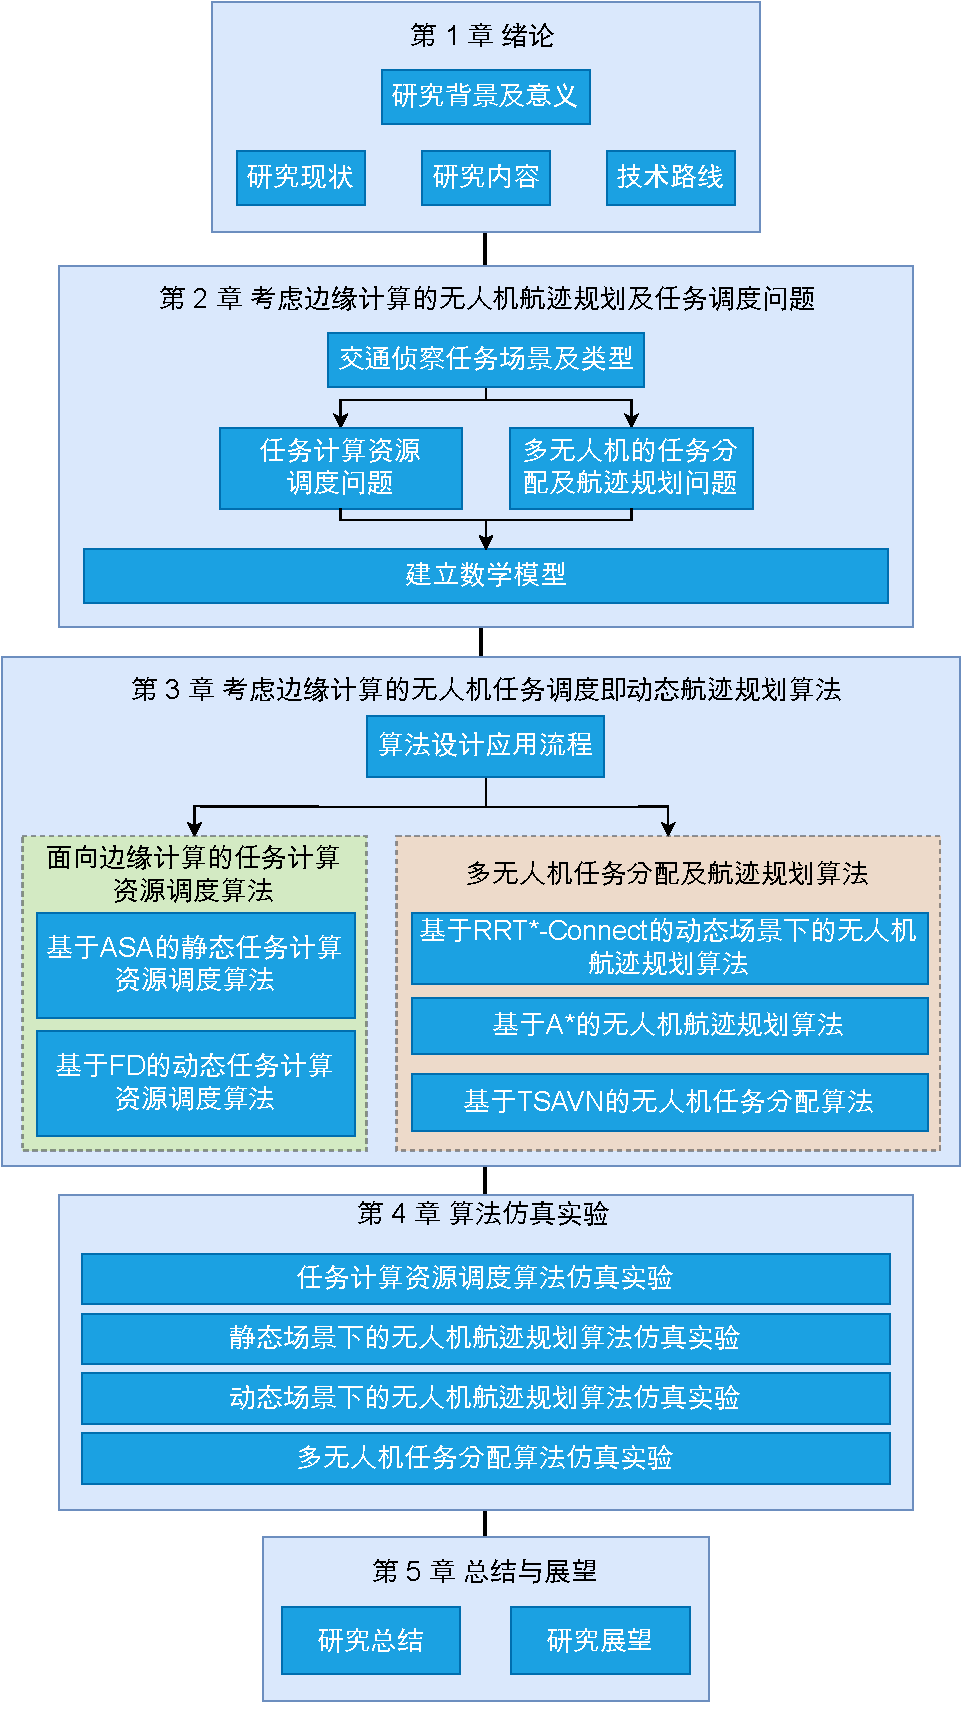
\includegraphics[width=0.7\textwidth]{./images/毕业设计技术路线结构图.drawio.pdf}
    \caption{毕业设计技术路线结构图}
    \label{fig:毕业设计技术路线结构图}
\end{figure}

\newpage


%!\mathbf{T}EX root = ../../csuthesis_main.tex
\chapter{考虑边缘计算的无人机航迹规划及任务调度问题}

\section{问题描述及场景设置} \label{sec:description}

\subsection{问题描述}

在交通及交通相关领域中,因为无人机具备隐蔽性好、机动性强、灵活性强,部署容易和应用范围广等特点,可以通过无人机的使用来一定程度上代替人工来完成所需的侦察任务,例如在铁路系统中对铁轨健康状况的检查、事故现场的侦察勘探、高速公路上的交通巡逻任务(见图~\ref{fig:无人机在高速公路上执行交通巡逻任务})等,因此,基于无人机的交通侦察应用逐渐具备了可行性与实用性。

\begin{figure}[!htbp]
    \centering
    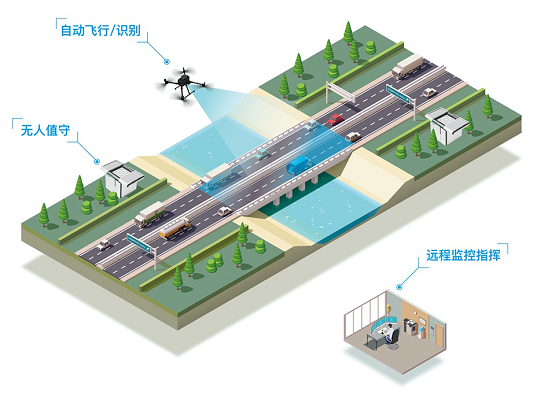
\includegraphics[width=0.7\textwidth]{images/无人机交通侦察应用场景.png}
    \caption{无人机在高速公路上执行交通巡逻任务}
    \label{fig:无人机在高速公路上执行交通巡逻任务}
\end{figure}

本文所研究的问题内容为考虑边缘计算的无人机航迹规划及任务调度问题,为方便讨论,本文将无人机需要执行的侦察任务分为两个部分(见图~\ref{fig:无人机侦察任务组成结构}),分别为收集型任务和计算型任务,其关系如图~\ref{fig:无人机侦察任务关系}所示。收集型任务主要与无人机的摄像设备以及储存设备有关,因此必须由无人机来完成,且该种任务的完成时间是可知的;而计算型任务则需要用到大量算力,若全靠无人机进行计算,则会使得无人机的续航大幅下降,从而使得无人机交通侦察系统效率大幅降低,而全由服务器进行计算,则容易因数据大量同时传输而造成网络拥堵等现象,同样降低了无人机交通侦察系统的效率。

\begin{figure}[!htbp]
    \centering
    \begin{subfigure}[t]{0.4\textwidth}
        \captionsetup{justification=centering}
        \begin{minipage}[b]{\linewidth}
            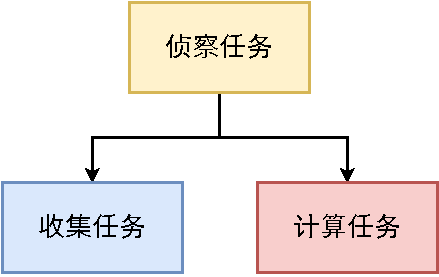
\includegraphics[width=\textwidth]{images/无人机侦察任务组成.pdf}
            \caption{无人机侦察任务组成结构}
            \label{fig:无人机侦察任务组成结构}
        \end{minipage}
    \end{subfigure}
    \begin{subfigure}[t]{0.75\textwidth}
        \captionsetup{justification=centering}
        \begin{minipage}[b]{\linewidth}
            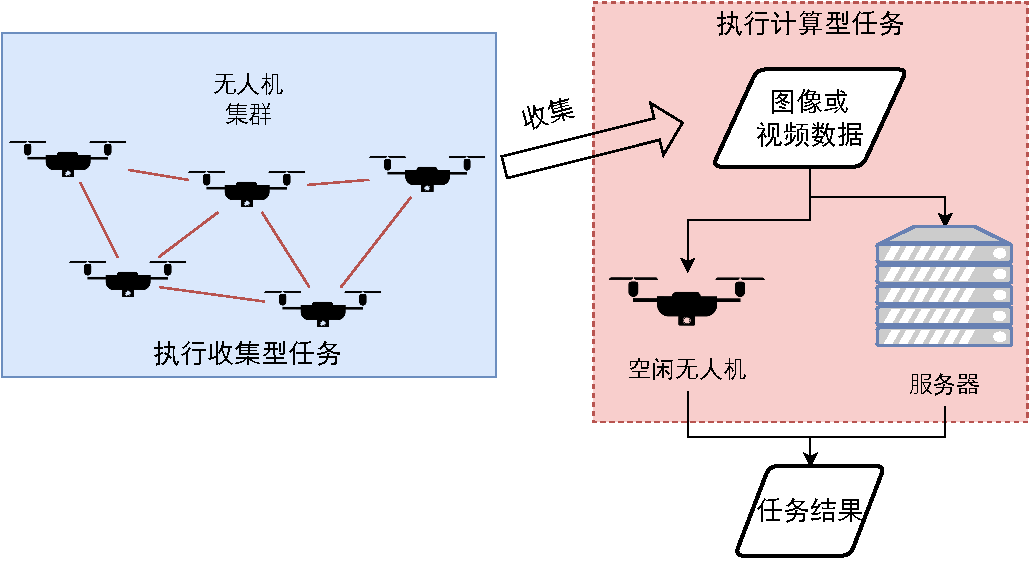
\includegraphics[width=\textwidth]{images/无人机侦察任务关系.pdf}
            \caption{无人机侦察任务关系}
            \label{fig:无人机侦察任务关系}
        \end{minipage}
    \end{subfigure}

    \caption{无人机交通侦察任务组成及关系}
    \label{fig:无人机交通侦察任务组成及关系}
\end{figure}

\begin{figure}[!htbp]
    \centering
    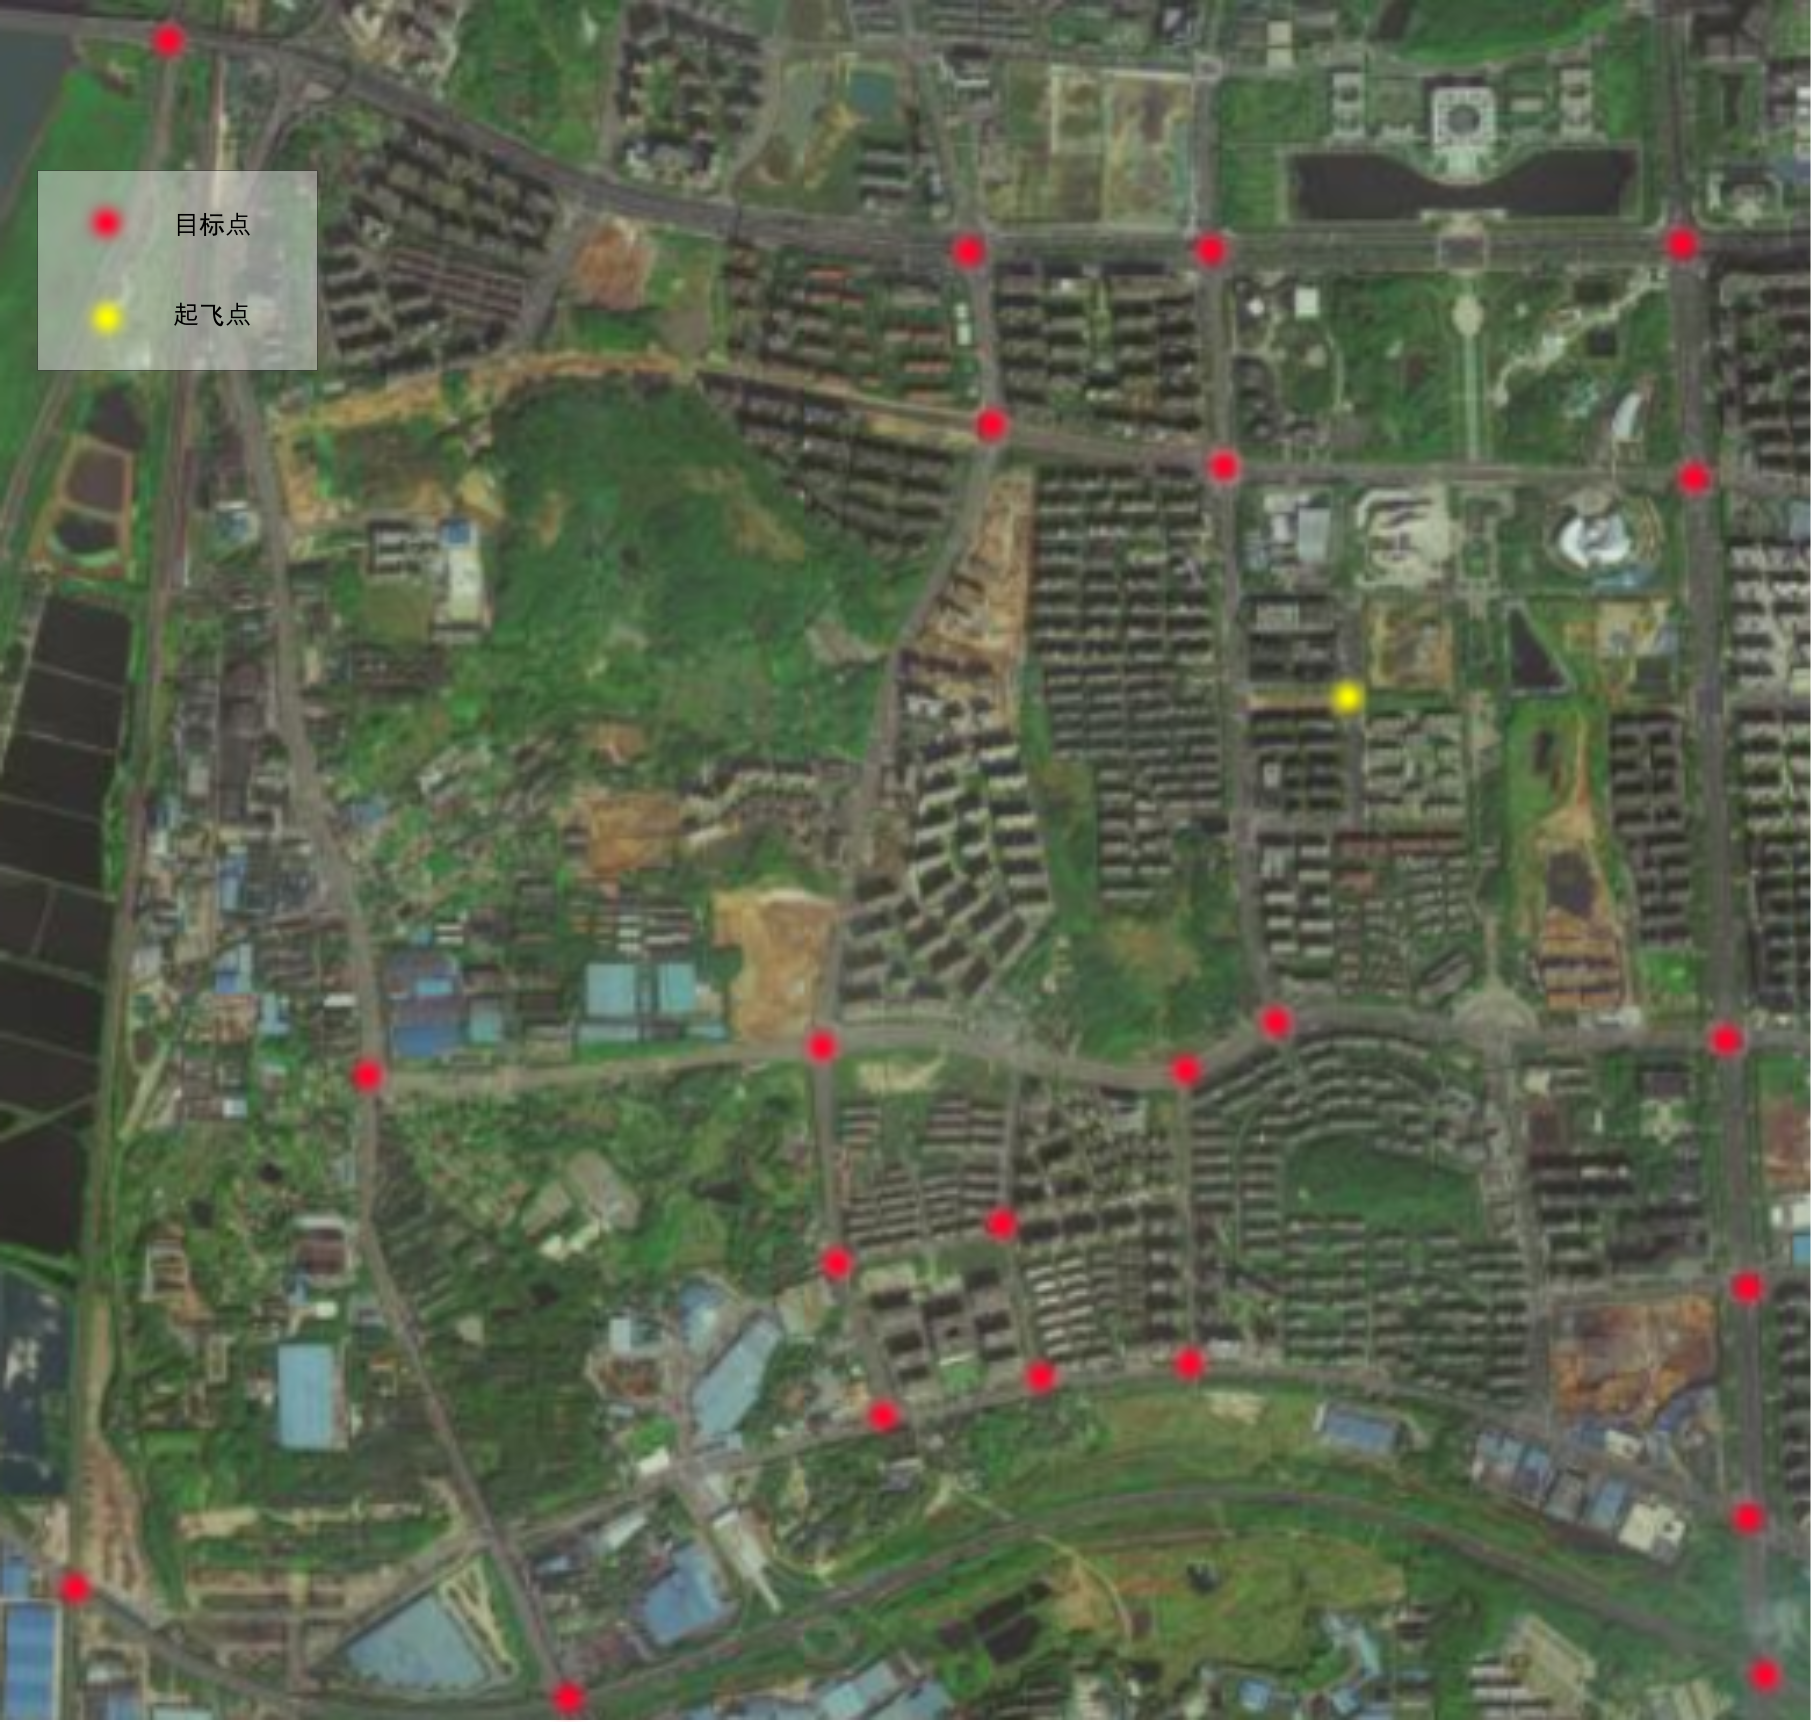
\includegraphics[width=0.7\textwidth]{./images/示例地图}
    \caption{示例地图信息}
    \label{fig:示例地图信息}
\end{figure}

为便于理解上述概念,此处不妨以侦察城市中道路交叉口当前的道路拥堵情况的侦察任务为例,可以将其分解为对该交叉口拍照或录制视频来收集当前道路情况的信息的收集型任务,以及对上述收集到的信息通过神经网络等方法进行计算得出当前该交叉口的道路拥挤情况的计算型任务。对于某个区域而言,存在着22个可能出现拥堵的交叉口(见图\ref{fig:示例地图信息}),需要使用一定数量的无人机来对每个交叉口拥堵情况进行数据收集,在每个任务的数据收集完成后,按照计算资源分配方案将任务数据通过网络通信等方式传输至地面端或边缘端中进行计算,得出各个交叉口拥挤情况后采取相应的措施。

那么基于上述内容,该问题的整体框架如图~\ref{fig:研究问题整体框架}所示,具体流程如下:

\begin{enumerate}[label=(\arabic*)]
    \item {当上级下达指令后,位于地面端的服务器根据任务信息以及地图信息,得到无人机的任务分配方案,包含所需无人机的数量、各无人机所要执行的需进行数据的采集与收集的收集型侦察任务以及相应的飞行航迹;}

    \item {同时服务器根据任务信息、服务器的计算资源以及无人机的计算资源,得到考虑边缘计算下的计算资源分配方案,来安排执行各计算型任务的设备;}

    \item {之后根据得到的无人机的收集型任务分配方案,将对应指令传输至无人机集群中,无人机根据接受到的指令进行飞行控制;}

    \item {在无人机按照飞行航迹进行飞行时,若飞行航迹中存在与航迹冲突的障碍物,那么需要实时对航迹进行修订,使得无人机能够在与障碍物发生碰撞之前对障碍物进行回避;}

    \item {在无人机到达目标点并采集完任务数据后,按照计算资源分配方案将任务数据通过网络通信等方式传输至地面端或边缘端中进行计算;}

    \item {最后根据计算所得的侦察任务结果采取对应的措施。}
\end{enumerate}

\begin{figure}[!htbp]
    \centering
    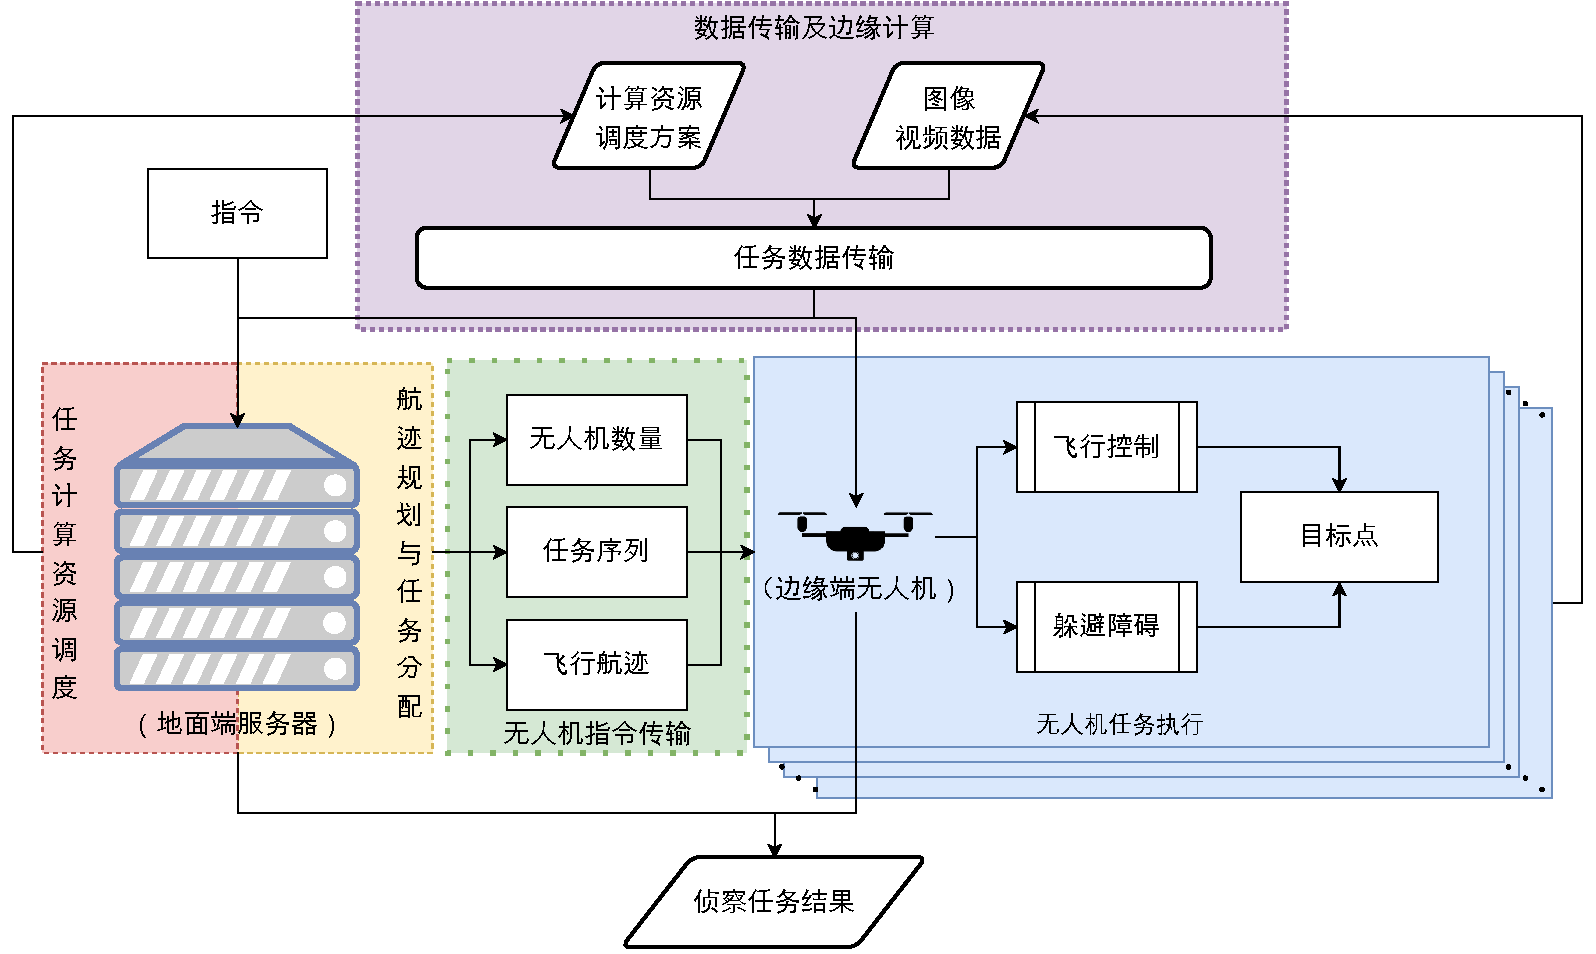
\includegraphics[width=\textwidth]{images/毕设问题框架.pdf}
    \caption{本文研究问题整体框架}
    \label{fig:研究问题整体框架}
\end{figure}

其中数据与指令的传输不在本文的研究范围内,因此本文将考虑边缘计算的无人机航迹规划及任务调度问题分为两个子问题,分别为面向边缘计算的任务计算资源调度优化问题、多无人机的航迹规划及任务分配问题。

\begin{figure}[!htbp]
    \centering
    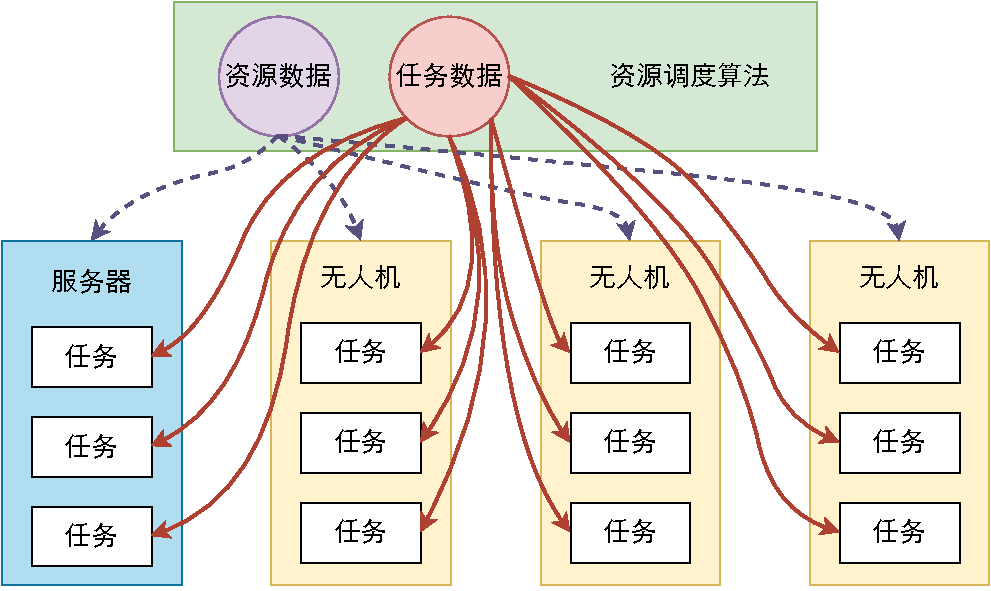
\includegraphics[width=0.7\textwidth]{images/资源调度算法.pdf}
    \caption{资源调度算法示意图}
    \label{fig:资源调度算法示意图}
\end{figure}

\begin{figure}[!htbp]
    \centering
    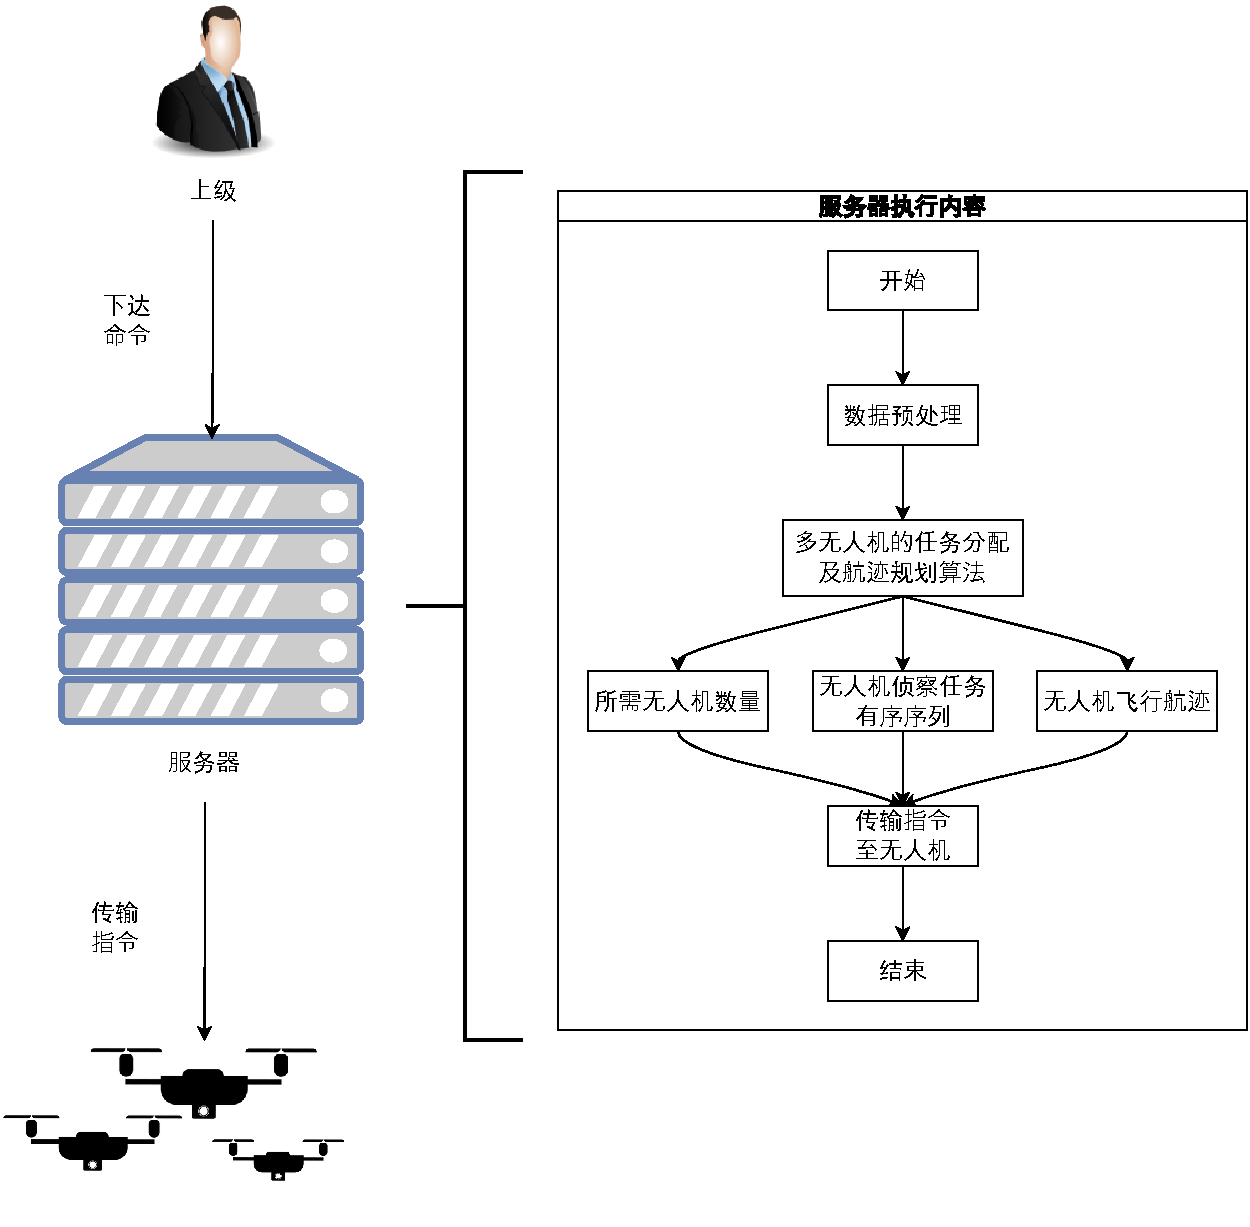
\includegraphics[width=0.9\textwidth]{images/多无人机的任务分配及航迹规划流程.pdf}
    \caption{多无人机的航迹规划及任务分配流程}
    \label{fig:多无人机的航迹规划及任务分配流程}
\end{figure}

任务计算资源的调度优化问题是在有限的计算资源及设备的情况下,通过一定的算法生成任务计算资源调度方案来安排计算设备完成指定的计算型任务,使得整个系统的成本较低,具备实用性的问题。因为无论是无人机集群还是服务器,其计算资源存在着一定的上限,而过多的布置无人机或服务器的数量,虽然能够确保所有计算任务都能够及时准确地完成计算,但会极大增加系统的成本,且有非常严重的资源浪费,而对计算资源进行充分地利用,能极大降低应用成本,提高系统的可行性,因此,在有限计算资源下对任务计算资源进行调度优化十分重要。对于整个系统而言,由于侦察任务有不同的种类,每个种类对于计算资源的要求各有不同,而无人机的计算资源,无论是可用CPU核心数还是可用内存,都与服务器存在着较大的差异,因此会存在着对于不同的侦察任务,其在不同设备的计算完成时间不一致的现象。与此同时,由于无人机与无人机、无人机与服务器之间是通过无线通信技术进行交流,因此还会存在着诸如通信延迟、传输丢包等通信问题,如何处理这些问题也是解决任务计算资源的调度优化问题中极为重要的内容。本文则提出一种具备负载均衡的面向边缘计算的任务计算资源分配算法(如图~\ref{fig:资源调度算法示意图}中的资源调度算法),根据设备的计算资源情况以及任务的需求情况,将不同的任务分配至无人机与服务器计算,合理有效地对计算资源进行分配。

由于无人机的计算功率,即是否进行对侦察任务数据的计算、计算所耗费的时间等,都会影响到无人机飞行的续航时间,而这不利于本章算法所涉及的资源分配问题的解决,同时也会对另外两个问题产生影响。因此,本章假定无人机的续航时间为可容许的最小续航时间,而剩余的续航时间所对应的计算资源则供给给可能需要进行计算的计算型侦察任务的数据。

如图~\ref{fig:多无人机的航迹规划及任务分配流程}所示,多无人机的航迹规划及任务分配问题是在给定收集型任务信息、地图信息后,由服务器根据所给信息,在尽可能短的时间内使用一定的算法确定完成任务所需的无人机数量、各无人机所执行的最优侦察任务有序序列、各无人机执行任务序列的最优飞行航迹,以便控制无人机完成所给的侦察任务的问题。

\subsection{场景设置}

本文以无人机群在城市环境中低空飞行,完成指定区域的目标识别任务、目标搜索任务等侦察任务为研究的应用场景。为简化整体问题便于研究,本文设定执行侦察任务所用无人机为同一型号的旋翼无人机,环境为存在障碍物高低差且障碍物数量较多、较为复杂的城市环境作为测试场景。

\section{模型假设}

为了能够集中力量研究主要问题,确定研究问题的边界,便于开展问题的研究,在不影响模型建立和求解算法的基础上,本文对考虑边缘计算的无人机航迹规划及任务调度问题提出下列合理的假设以简化模型:

\begin{enumerate}
    \item {无人机应用场景中,所有的障碍物均以长方体进行拟合;}

    \item {服务器具有的计算能力和计算资源均强于无人机,使得在计算同一侦察任务的数据使服务器能够以更快的速度完成任务以及同时能够完成更多任务;}

    \item {通信传输的延迟不会受到除了设备间的欧式距离以外的因素的影响;}

    \item {无人机与无人机、无人机与服务器之间的网络延迟具备可预测性,即能够根据无人机位置、通信时间等预测设备间的网络延迟;}

    \item {无人机携带的传感器能够实时感知所在环境的障碍物信息,能够获取无人机与障碍物的距离等所需信息;}

    \item {无人机能够自行处理部分侦察任务的数据,但计算时间会长于服务器计算时间;}

    \item {服务器拥有的地图数据为最新数据,与现实地图不存在较大的差距变化,例如现实中存在的大楼在地图数据中显示为空地,仅存在微小的变化,例如大楼外部的空调外机;}

    \item {无人机进行转向活动时耗费的时间不计;}

    \item {同一任务在相同设备上运行时间具备可预测性,即能够根据任务类型、任务所需内存及设备类型预测该任务在该设备下完成计算所需时间;}

    \item {无人机和服务器都可以同时执行任意数量的任务且不会影响它们的运算速度。}
\end{enumerate}

\section{符号定义}

表~\ref{tab:数学符号及意义}为小节~\ref{sec:math_model}中的数学模型所使用的数学符号:

\begin{longtable}{c C{0.8\textwidth}}
    \caption{数学符号及意义} 
    \label{tab:数学符号及意义} \\
    \hline
        \textbf{符号} & \textbf{意义}\\
    \hline
        \( N \) & 无人机数量 \\
        \( \mathbf{O} \) & 障碍物集合 \\
        \( \ell_\text{max} \) & 无人机最大航程 \\
        \( C_k \) & 第\( k \)台无人机的航迹坐标 \\
        \( d(C_k) \) & 根据第\( k \)台无人机的航迹坐标计算得出的飞行航程 \\
        \( \mathbf{J} \) & 任务集合 \\
        \( J \) & 任务数量 \\
        \( i \) & 第\( i \)个任务 \\
        \( \mathbf{T} \) & 任务类型集合 \\
        \( \mathbf{T}_i \) & 第\( i \)个任务的类型 \\
        \( k \) &  第\( k \)台设备 \\
        \( \mathbf{M} \) & 设备集合 \\
        \( M \) & 设备数量 \\
        \( G_k \) &  第\( k \)台设备为地面端,0则不是,1则是 \\
        \( L_k \) & 第\( k \)台设备的最大内存 \\
        \( W_i \) & 执行第\( i \)个任务所需内存 \\
        \( D_{i k} \) & 第\( i \)个任务上传至第\( k \)个设备的通信延迟,不需要上传时为\( 0 \) \\
        \( X_{i k} \) & 第\( i \)个任务是否由第\( k \)个设备处理 \\
        \( F_{i k} \) & 第\( i \)个任务上传至第\( k \)个设备的上传速度,不需要上传时为\( \infty \) \\
        \( P(W_i, \mathbf{T}_i, G_k) \) & 根据第\( i \)个任务的所需内存和任务类型预测在第\( k \)个设备中开始处理到处理完成所需的时间的函数 \\
        \( t_{i k} \) & 第\( i \)个任务从开始执行到在第\( k \)个设备中处理到执行完成总共的时间 \\
        \( S_{i} \) & 第\( i \)个任务开始执行的时间 \\
        \( C_{i} \) & 第\( i \)个任务执行完成的时间 \\
        \( C_{\text{max}} \) & 所有任务中最后完成执行的任务的完成时间 \\
    \hline
\end{longtable}

\section{数学模型} \label{sec:math_model}

本小节根据小节~\ref{sec:description}中对无人机交通侦察动态规划问题进行分解后的问题分别建立任务计算资源调度模型(见小节~\ref{sec:resouce_scheduling_model})、多无人机航迹规划及任务分配模型(见小节~\ref{sec:assignment_model})。

\subsection{任务计算资源调度模型} \label{sec:resouce_scheduling_model}

\begin{equation}
    \min F_1 = (C_{\text{max}}, C_{\text{max}} \cdot M - \sum^J_{i} \sum^M_{k} t_{ik} X_{i k})  \label{eq:target1}
\end{equation}

\begin{equation}
    C_{\text{max}} = \max(C_{i}) \label{eq:target_mean1}
\end{equation}

\begin{equation}
    C_{i} = S_{i} + \sum_{k \in [1, M]} t_{ik} X_{ik} \label{eq:completion_time3}
\end{equation}

\begin{equation}
    t_{ik} = 2 D_{ik} + \frac{W_i}{F_{ik}} + P(W_i, \mathbf{T}_i, G_k) \label{eq:compute_time3}
\end{equation}

s.t.

\begin{equation}
    \sum_{i \in [1, J]} W_i X_{ik} < L_k, \forall_{t \in [0, C_{\text{max}}]} \forall_{k \in [1, M]} \label{eq:mem_restrant3}
\end{equation}

\begin{equation}
    \sum_{k \in [1, M]} X_{ik} = 1, \forall_{i \in [1, J]} \label{eq:only_one3}
\end{equation}

\begin{equation}
    X_{ik} = \{0, 1\}, \forall_{i \in [1, J], k \in [1, M]} \label{eq:integer_restrant3}
\end{equation}

\begin{equation}
    \sum_{i \in [1,  J]} \sum_{k \in [1, M]} X_{i k} = J \label{eq:all_mission3}
\end{equation}

\begin{equation}
    P(W_i, \mathbf{T}_i, G_k) > 0, \forall_{i \in [1, J], k \in [1, M]} \label{eq:predict_function3}
\end{equation}

\begin{equation}
    C_{i} > S_{i} \ge 0, \forall_{i \in [1, J], k \in [1, M]} \label{eq:time_restrant3}
\end{equation}

\begin{equation}
    D_{ik}, F_{ik}, L_{i}, W_{i}, t_{ik}, G_{k} > 0, \forall_{i \in [1, J], k \in [1, M]}, G_{k} \in \mathbb{Z} \label{eq:variable_restrant3}
\end{equation}

其中,式~\ref{eq:target1}为模型的目标函数,该目标值的含义如表~\ref{tab:数学符号及意义}中所示,即任务完成时间\( C_{\text{max}} \)最短、设备空闲时间\( C_{\text{max}} \cdot M - \sum^J_{i = 1} \sum^M_{k = 0} t_{ik} X_{i k} \)最少,而设备空闲时间最少是为了确保设备的资源利用率,使得本文所提出的算法具备负载平衡的功能,其中任务完成时间的计算方式如式~\ref{eq:target_mean1}所示;而对于第\( i \)任务的完成时间\( C_{i} \),则由式~\ref{eq:completion_time3}中所示,由任务的开始执行时间\( S_{i} \)与决策确定的完成所需时间\( \sum_{k \in [1, M]} t_{ik} X_{ik} \)之和决定;而对于第\( i \)个任务在第\( k \)台设备上的完成所需时间\( t_{ik} \),则由式~\ref{eq:compute_time3}所决定,其中分别为上传延迟\( D_{i k} \)、上传时间\( \frac{W_i}{F_{i k}} \)、计算时间\( P(W_i, \mathbf{T}_i, G_k) \)和下载延迟\( D_{i k} \)所决定。

在上述基础上,本文对整个场景进行了约束,其中式~\ref{eq:mem_restrant3}确保在任意时刻下,任意设备所执行的任务所需内存总和不超过该设备最大可用内存;式~\ref{eq:only_one3}和~\ref{eq:integer_restrant3}确保每一个任务只会且只能由一台设备所执行;式~\ref{eq:all_mission3}确保每一个任务都会被完成;式~\ref{eq:predict_function3}是确保对任务完成所需时间的预测在一个符合实际的范围;式~\ref{eq:variable_restrant3}则式对各个变量进行约束。

\subsection{多无人机航迹规划及任务分配模型} \label{sec:assignment_model}

\begin{equation}
    \min F_2 = (\sum^N_{k=1} d(C_k), N)  \label{eq:target2}
\end{equation}

s.t.

\begin{equation}
    C_k \notin \mathbf{O}, \forall_{k \in [1, N]} \label{eq:route_constrain}
\end{equation}

\begin{equation}
    d(C_k) \le \ell_\text{max} , \forall_{k \in [1, N]} \label{eq:route_length_constrain}
\end{equation}

\begin{equation}
    C_1 \cap C_2 \cap \ldots \cap C_N = \emptyset \label{eq:crash_constrain}
\end{equation}

其中,式~\ref{eq:target2}表示优化目标为无人机数量最少,且无人机的飞行航程之和最小;式~\ref{eq:route_constrain}为
无人机与障碍物的飞行避撞约束,即无人机在飞行航迹中任意一点均不与障碍物接触,从而避免飞行过程中发生无人机因与障碍物碰撞而损毁的情况;
式~\ref{eq:route_length_constrain}为无人机的航程约束,确保每一无人机飞行航迹的飞行航程均不超过其最大航程,从而
避免无人机因续航耗尽导致的损毁;式~\ref{eq:crash_constrain}无人机与无人机的飞行避撞约束,
即无人机在飞行航迹中任意一点均不与其他无人机接触,从而避免飞行过程中发生无人机因与其他无人机碰撞而损毁的情况。

\section{本章小结}

本章主要对无人机航迹规划及任务调度问题进行具体描述和分析,同时将该问题分解成了两个子问题,分别是任务计算资源的调度优化问题、多无人机的航迹规划及任务分配问题,并在提出合理假设和数学符号的基础上,分别建立任务计算资源的调度优化问题、多无人机的航迹规划及任务分配问题的数学模型,并对各个模型的目标函数及约束条件进行了说明。

\newpage


%!TEX root = ../../csuthesis_main.tex
\chapter{考虑边缘计算的无人机航迹规划及任务调度算法}

\section{算法设计应用流程}

\begin{figure}[!htbp]
    \centering
    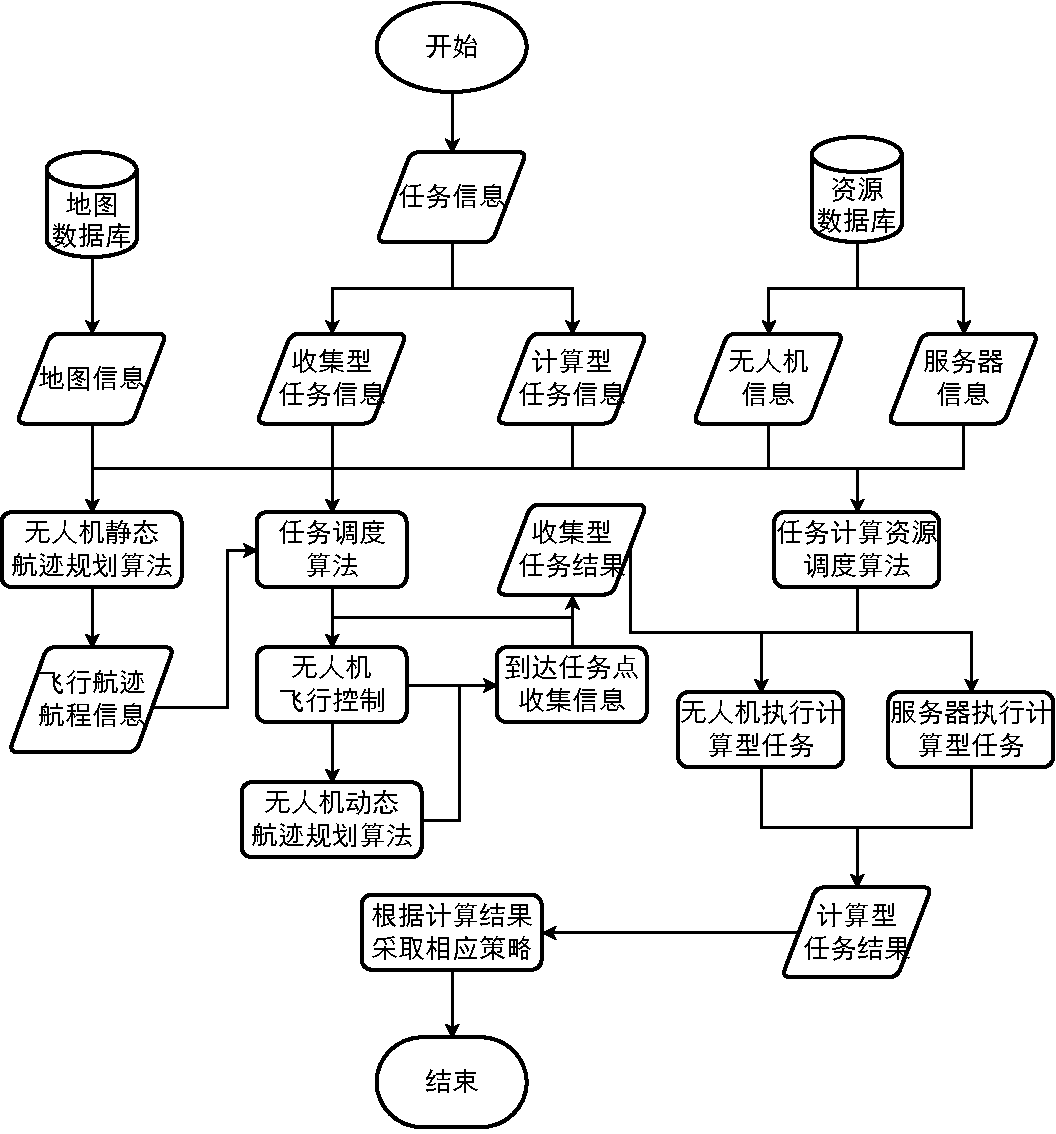
\includegraphics[width=0.9\textwidth]{images/算法设计应用流程.pdf}
    \caption{算法设计应用流程}
    \label{fig:算法设计应用流程}
\end{figure}

本文针对无人机航迹规划及任务调度问题所设计的算法的应用流程如下,首先将所给的任务信息分解成收集型任务信息和计算型任务信息,然后服务器根据收集型任务信息、从资源数据库中得到的无人机信息、从地图数据库中得到的地图信息,放入静态场景下的无人机航迹规划算法中,得到各点间的无人机飞行航迹和航程的对应信息,再将以上信息以及收集型任务信息放入任务调度算法,得到所需无人机的数量、每个无人机需要执行的收集型任务有序序列、无人机飞行航迹等信息;同时服务器再根据计算型任务信息、无人机信息和服务器信息通过任务计算资源调度算法,为每一个计算型任务分配对应的计算设备;然后无人机根据所给的任务序列和飞行航迹进行飞行控制,若遇到航迹中的存在的障碍物则使用动态场景下的航迹规划算法修订航迹来回避障碍物,在到达任务点后执行收集型任务,在完成后将收集得到的任务结果传输至执行该收集型任务对应的计算型任务的设备中进行计算,在计算型任务完成后,便能够根据任务结果采取相应的措施,流程如图~\ref{fig:算法设计应用流程}所示。

\section{面向边缘计算的任务计算资源调度算法}

由于生成任务计算资源调度方案需要无人机的航程信息,而在无人机飞行过程中,随时可能因为出现与原定航迹相冲突的障碍物而对航迹进行修订,进而使其航程信息发生变化,因此在解决该问题时,本文先将该问题分为无人机尚未接收到指令开始执行任务前的静态场景以及无人机开始执行任务,但由于中途进行了避障操作而使得原本的资源调度方案需要重新生成的动态场景。在静态场景中,由于不需要在很短时间内给出调度方案,因而计算资源调度方案的质量比算法计算时间更为重要;而在动态场景中,由于场景信息不断发生变动,为避免计算资源调度方案的生成时间过长导致无人机的数据传输需要进行等待,进而导致系统效率下降,此时算法的运行时间更为重要。

基于以上分析,本文提出的面向边缘计算的任务计算资源调度算法共包含两个算法,分别是用于求解静态场景的参数自适应的模拟退火算法(Adaptive Simulated Annealing, ASA)以及用于求解动态场景的快速决策算法(Fast Decision-making Algorithm, FD)。

\subsection{基于ASA的静态场景下的任务计算资源调度算法}

本算法是在传统SA算法的基础上,对其进行了邻域结构以及参数方面的改进。

\subsubsection{邻域结构设计} \label{sec:neighbor_design}

由于需要执行的任务数是一定的,且一个任务仅由一个设备进行处理计算,而一个设备可能需要处理多个任务,因此可以简单地使用一个数组来作为算法的解,其中数组的元素对应的位置为任务的序号、数组的元素为设备的序号,以此来设计本文所使用的邻域结构。

第一种邻域结构为任务交换邻域结构,如图~\ref{fig:任务交换邻域结构}所示,具体操作流程如下:

\begin{enumerate}[label=(\arabic*)]
    \item {选取待交换的两个任务\(M_1\)、\(M_2\);}
    \item {获取用于处理任务\(M_1\)与\(M_2\)的设备\(D_1\)与\(D_2\);}
    \item {交换处理这两个任务的设备,即原本由设备\(D_1\)处理任务\(M_1\),设备\(D_2\)处理任务\(M_2\),
    变为由设备\(D_2\)处理任务\(M_1\),设备\(D_1\)处理任务\(M_2\)。}
\end{enumerate}

\begin{figure}[!htbp]
    \centering
    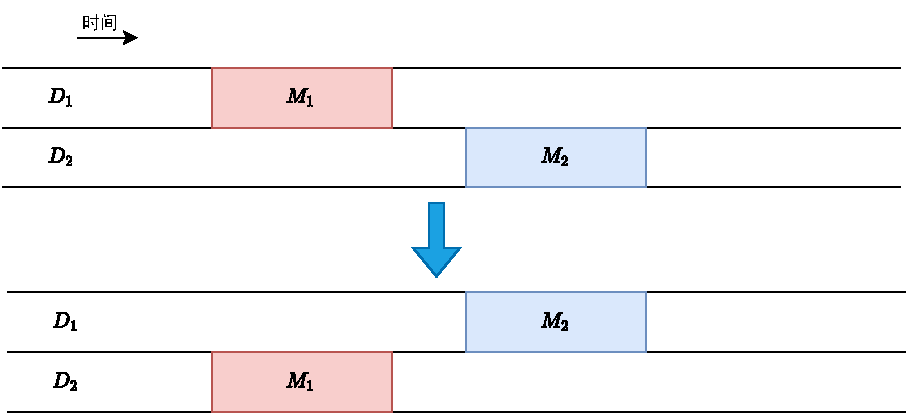
\includegraphics[width=0.7\textwidth]{images/基于边缘计算的任务资源调度算法_任务交换算子.pdf}
    \caption{任务交换邻域结构}
    \label{fig:任务交换邻域结构}
\end{figure}

第二种邻域结构为无人机间任务转移邻域结构,如图~\ref{fig:无人机间任务转移邻域结构}所示,具体操作流程如下:

\begin{enumerate}[label=(\arabic*)]
    \item {选取任务\(M_1\)、\(M_3\);}
    \item {获取用于处理任务\(M_1\)与\(M_3\)的无人机设备\(U_1\)与\(U_2\);}
    \item {将任务\(M_1\)分配给无人机设备\(U_2\)处理,即原本由无人机设备\(U_1\)处理任务\(M_1\),
    变为由无人机设备\(U_2\)处理任务\(M_1\)。}
\end{enumerate}

\begin{figure}[!htbp]
    \centering
    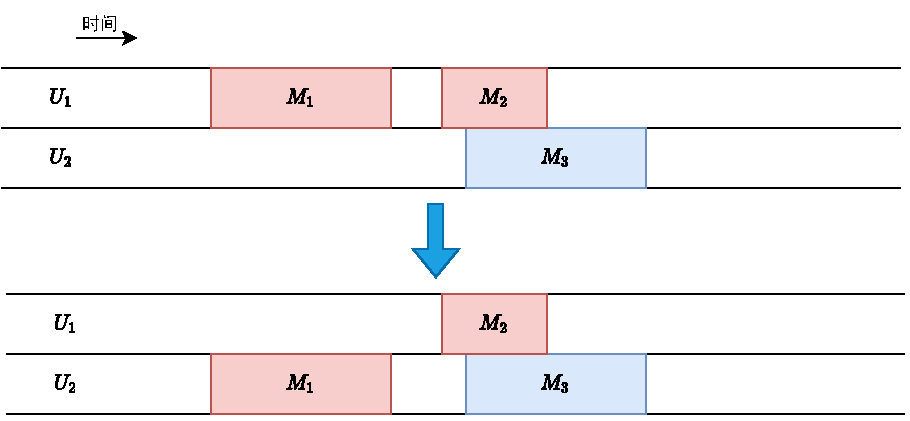
\includegraphics[width=0.7\textwidth]{images/基于边缘计算的任务资源调度算法_无人机间任务转移算子.pdf}
    \caption{无人机间任务转移邻域结构}
    \label{fig:无人机间任务转移邻域结构}
\end{figure}

第三种邻域结构为无人机向服务器转移任务邻域结构,如图~\ref{fig:无人机向服务器转移任务邻域结构}所示,具体操作流程如下:

\begin{enumerate}[label=(\arabic*)]
    \item {选取任务\(M_1\);}
    \item {获取用于处理任务\(M_1\)的无人机设备\(U\);}
    \item {将任务\(M_1\)分配给服务器设备\(C\)处理,即原本由无人机设备\(U\)处理任务\(M_1\),
    变为由服务器设备\(C\)处理任务\(M_1\)。}
\end{enumerate}

\begin{figure}[!htbp]
    \centering
    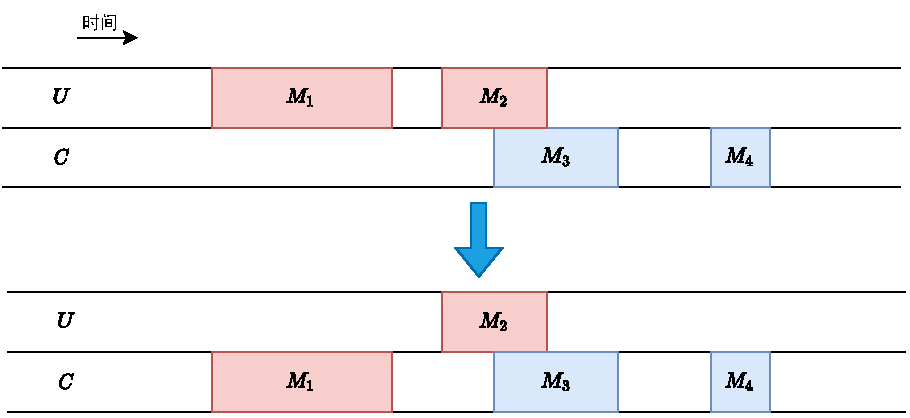
\includegraphics[width=0.7\textwidth]{images/基于边缘计算的任务资源调度算法_无人机向服务器转移任务算子.pdf}
    \caption{无人机向服务器转移任务邻域结构}
    \label{fig:无人机向服务器转移任务邻域结构}
\end{figure}

第四种邻域结构为服务器向无人机转移任务邻域结构,如图~\ref{fig:服务器向无人机转移任务邻域结构}所示,具体操作流程如下:

\begin{enumerate}[label=(\arabic*)]
    \item {选取由服务器处理的任务\(M_1\);}
    \item {获取无人机设备\(U\);}
    \item {将任务\(M_1\)分配给无人机设备\(U\)处理,即原本由服务器设备\(C\)处理任务\(M_1\),
    变为由无人机设备\(C\)处理任务\(M_1\)。}
\end{enumerate}

\begin{figure}[!htbp]
    \centering
    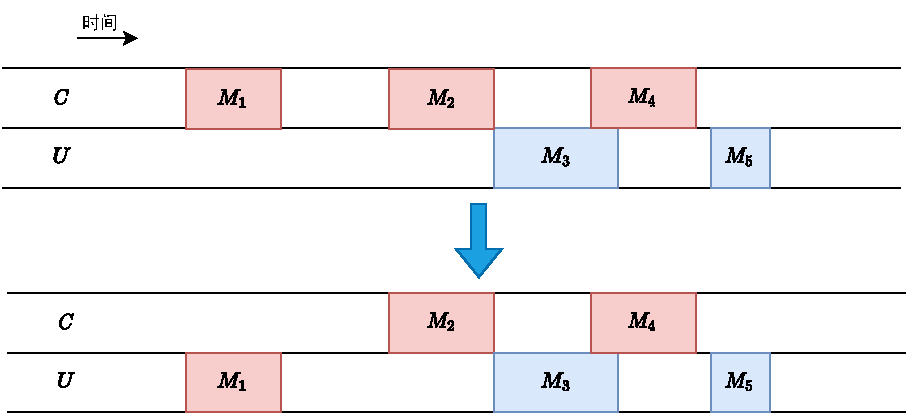
\includegraphics[width=0.7\textwidth]{images/基于边缘计算的任务资源调度算法_服务器向无人机转移任务算子.pdf}
    \caption{服务器向无人机转移任务邻域结构}
    \label{fig:服务器向无人机转移任务邻域结构}
\end{figure}

\subsubsection{自适应机制设计}

对于小节~\ref{sec:neighbor_design}中所述的邻域结构而言,在不同的情况下每个邻域结构的表现会存在差异,因此为使得算法性能更好,本文提出了基于优胜劣汰机制的邻域结构权重自适应机制,该机制能够使得表现优异的邻域结构在下次选择是被选到的机会更大,而表现较差的邻域结构则被选到的机会更小。

在算法初始化时,每个邻域结构的权重均初始化为1。在之后权重的迭代更新中,为了避免滚雪球现象,即某个邻域结构在连续非常多次表现优异后,即使此后该邻域领域的表现非常差,选择其他邻域结构也非常小,或是连续非常多次表现较差时,即使此后该邻域领域的表现非常优异,继续选择该邻域结构的概率非常小,因此在设计该机制时,本文根据生成的新解的质量与当前解的质量进行比较,此处引入\(w^r_i\)作为第\(i\)个邻域结构被第\(r\)次选中并计算完成后的权重,\(\Delta E\)为解的质量下降的值,那么有

\begin{equation}
    w^r_i = 
    \begin{aligned}
    \begin{cases}
        \bar{w^r} \quad &\text{if} \quad \Delta E > 0 \\
        0.8 \cdot w^{r-1}_i \quad &\text{if} \quad \Delta E < 0
    \end{cases} 
    \end{aligned}\nonumber
\end{equation}


另外,由于模拟退火算法在运行中会存在初期温度高,同时未达到局部最优解的情况,以及末期温度低,同时达到局部最优解的情况,导致其非更优解接受概率的利用程度不高,所以模拟退火算法的性能仍有待提高。

为提高模拟退火算法的性能,更充分地利用其跳出局部最优解的机制,此处采用了自适应温度机制取代了原有的温度机制。

此处引入\(r_{i}\)作为算法第\(i\)次运行后没有得到更优解的次数,即需要计算非更优解接受概率的次数,当直接得到了更优解时\(r_{i} = 0\),算法未运行时\(r_{0} = 0\),即

\begin{equation}
    r_i = 
    \begin{aligned} 
    \begin{cases}
        r_{i-1} + 1 \quad &\text{if} \quad \Delta E > 0\\
        r_{i-1} &\text{if} \quad \Delta E = 0 \\
        0 &\text{if} \quad \Delta E < 0
    \end{cases}
    \end{aligned}
    \nonumber
\end{equation}

同时使用迭代次数\(N\)来控制整个算法的逻辑。与模拟退火算法相比,其总的求解次数仅由\(N\)决定,而模拟退火算法的总求解次数为\(N \cdot \log_{r}\frac{T_{0}}{T_{\text{end}}}\)。

设定一个最低温度\(T_{\min}\),升温速率\(\rho\)以及温控参数\(\delta\),使得第\(i\)次计算温度\(T_{i}\)时使用如下公式:

\begin{equation}
    T_i = T_{\min} + \rho \cdot \ln (1 + \frac{r_i}{\delta})
    \nonumber
\end{equation}

如此便能够在能够寻求到最优解的情况下维持低温,在到达局部最优解、需要到达新的局部最优解时能够通过升高温度来跳出局部最优解,从而使算法具有更好的鲁棒性。

\subsection{基于FD的动态场景下的任务计算资源调度算法}

在计算资源调度的动态场景中,由于每个无人机有两种决策方式:将任务数据传输至地面端服务器,由地面端服务器进行计算;将任务数据传输至边缘端无人机,由边缘端无人机进行计算。

\begin{figure}[!htbp]
    \centering
    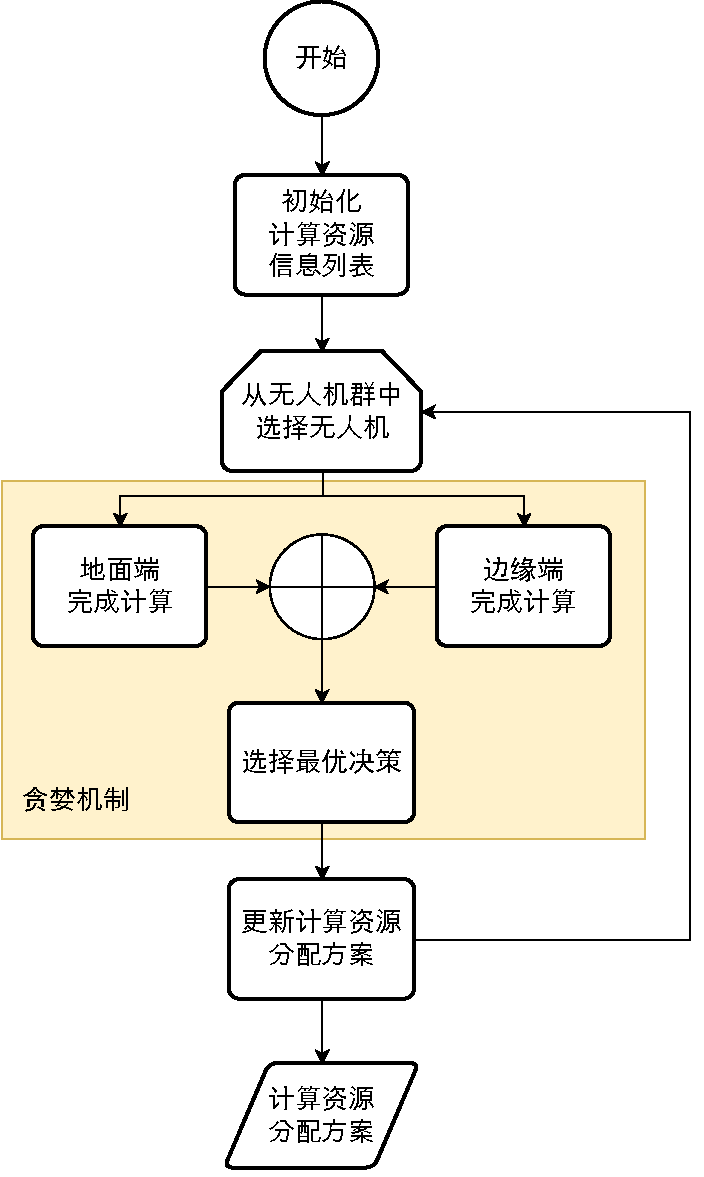
\includegraphics[width=0.6\textwidth]{./images/fd.pdf}
    \caption{FD算法流程图}
    \label{fig:FD算法流程图}
\end{figure}


因此,在满足算法生成的计算资源调度方案具有实用性的条件下,为使得算法的运行时间尽可能短,本算法在无人机决策时采用了贪婪机制(见图\ref{fig:FD算法流程图}),在对所有无人机进行遍历决策后,即可生成计算资源调度方案。

\subsection{算法流程图}

根据上述内容,本文提出的面向边缘计算的任务计算资源调度算法的运行流程如下,首先从对应数据库中获取当前的计算型侦察任务的具体信息以及无人机、服务器的计算资源的信息,在初始化算法参数后,根据以上信息生成初始解,然后进行一定次数的迭代;在每步迭代中,算法从任务交换邻域结构、无人机间任务转移邻域结构、无人机向服务器转移任务邻域结构、服务器向无人机转移任务邻域结构中选择一个进行当前解的邻域变动,得到优化结果,判断该优化结果与目前的最优解是否更优,若更优则保存,否则进行概率判断,按随机概率确定是否保存,保存则更新最优解,然后更新算法参数,直至迭代结束,在迭代结束后,即可得到当前任务的计算资源最优分配方案。总流程如图~\ref{fig:基于边缘计算的任务资源调度算法流程图}所示。

\begin{figure}[!htbp]
    \centering
    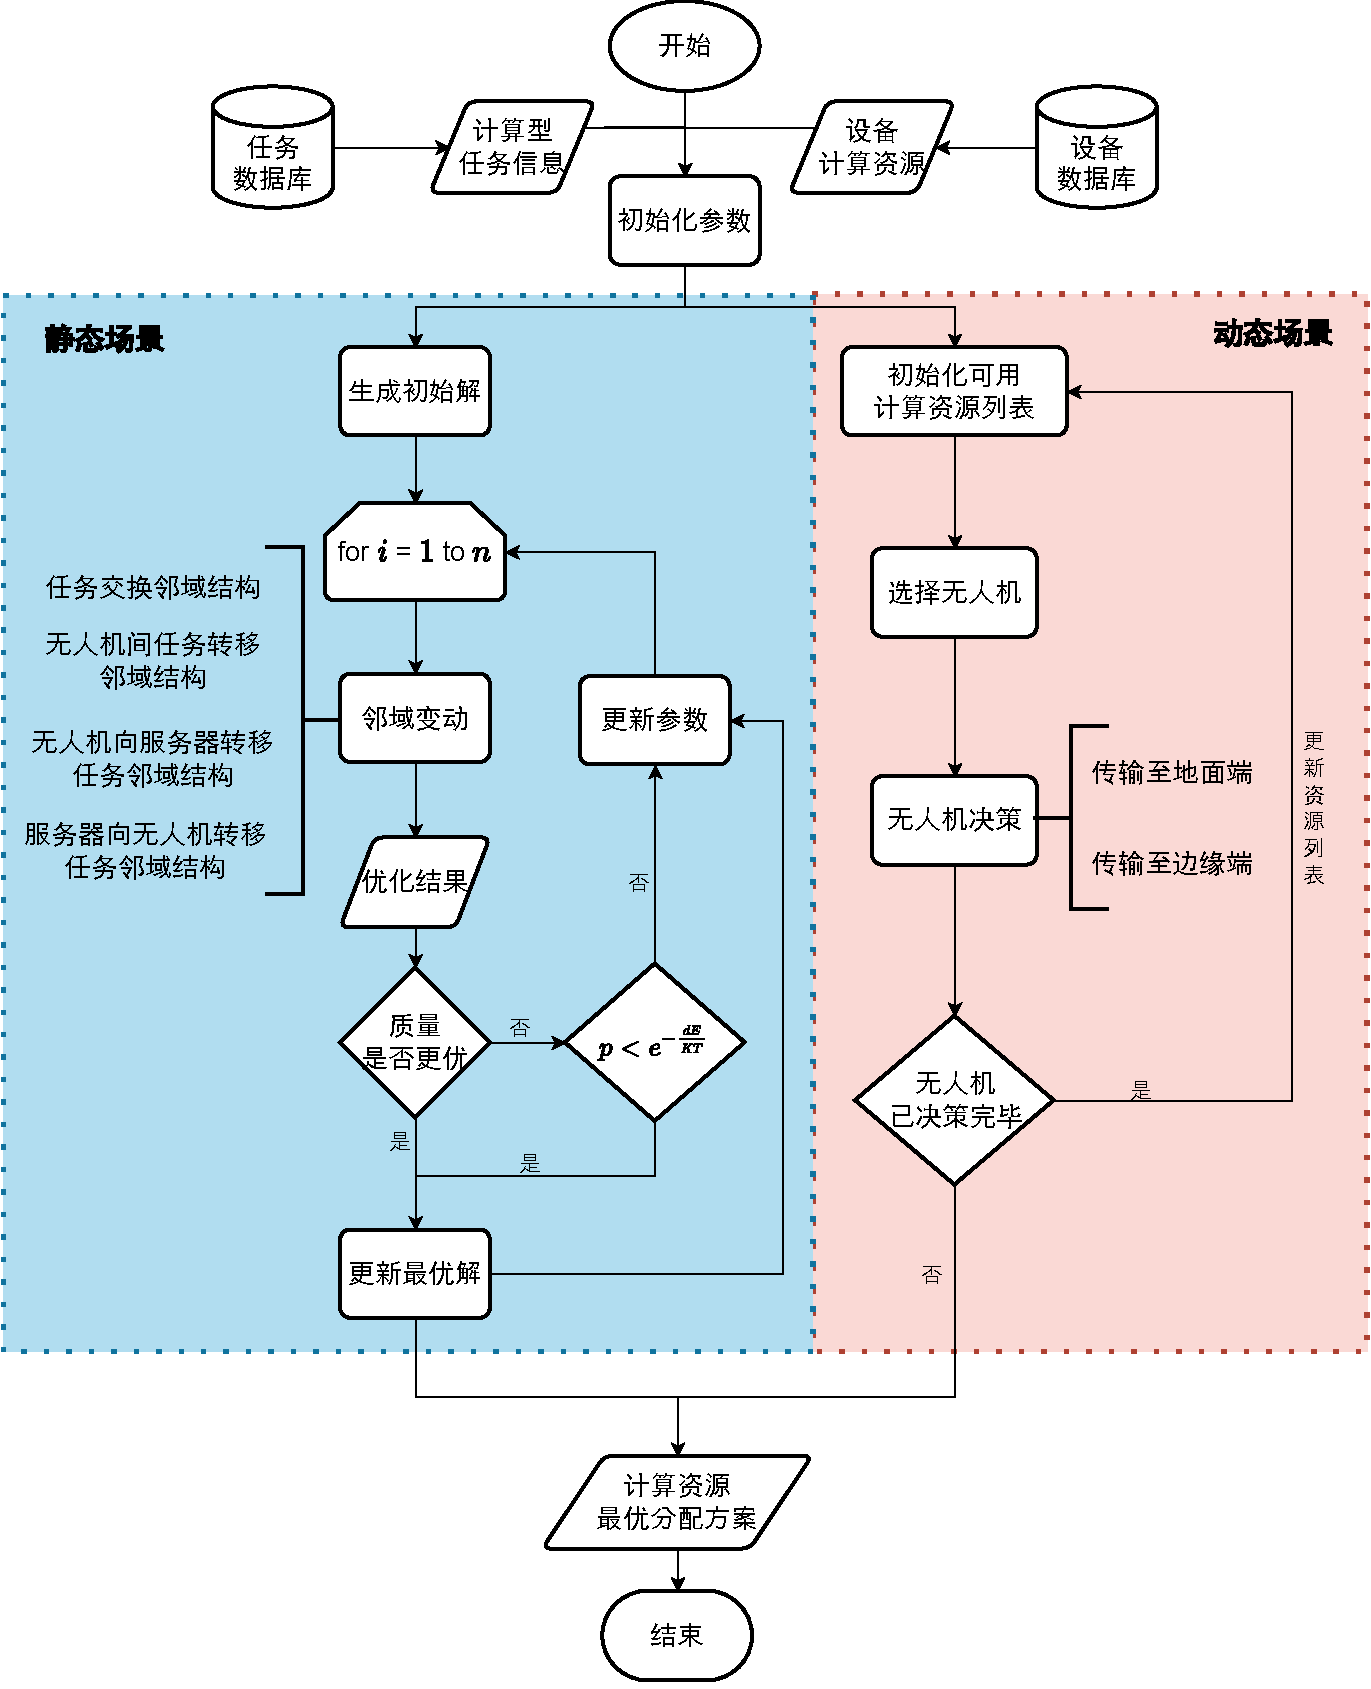
\includegraphics[width=\textwidth]{images/基于边缘计算的任务资源调度算法流程图.pdf}
    \caption{面向边缘计算的任务计算资源调度算法流程图}
    \label{fig:基于边缘计算的任务资源调度算法流程图}
\end{figure}



%!TEX root = ../../csuthesis_main.tex

\section{多无人机航迹规划及任务分配算法}

本节针对多无人机航迹规划及任务分配问题,构建了基于快速随机搜索树算法、A*算法、模拟退火算法、变邻域搜索算法的多无人机航迹规划及任务分配框架,该框架将多无人机航迹规划及任务分配问题划分为了无人机航迹规划阶段以及任务调度分配阶段,流程如图~\ref{fig:多无人机航迹规划及任务分配流程}所示,并针对这两个阶段,设计相应的算法。在无人机航迹规划阶段,提出了能够在静态场景下快速获得最优航迹的RRT*-Connect算法以及能够在动态场景下快速获得避障航迹的A*算法;在多无人机任务调度分配阶段,提出了基于模拟退火算法、变邻域算法以及温度自适应模拟退火算法\citep{wu2017SatelliteObservationSchedulinga}的变邻域结构搜索的温度自适应模拟退火算法(Temperature-adaptive Simulated Annealing Algorithm with Variable Neighborhood, TSAVN)。由RRT*-Connect生成无人机起飞点、任务点间的点与点的最优飞行航迹与航程,并利用生成的航程信息为TSAVN算法提供依据完成多无人机的任务调度。

\begin{figure}[!htbp]
    \centering
    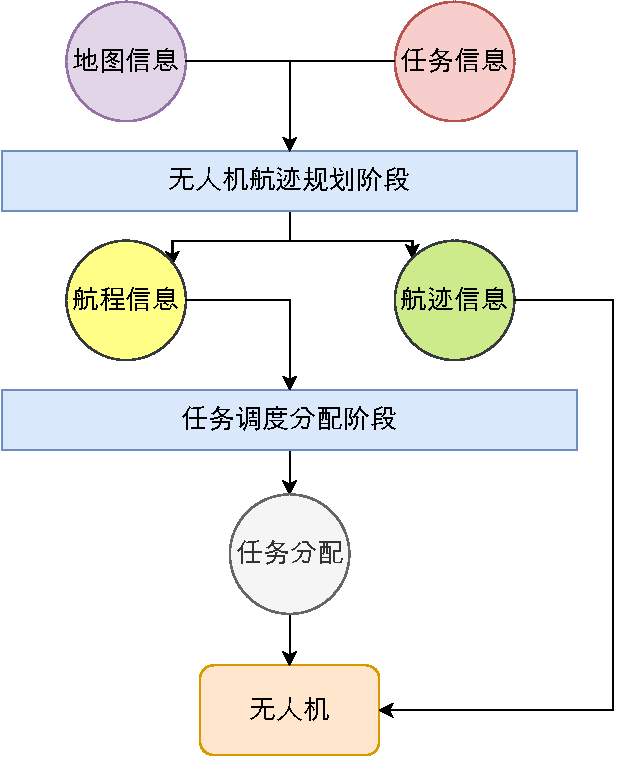
\includegraphics[width=0.5\textwidth]{images/多无人机任务分配及航迹规划流程.drawio.pdf}
    \caption{多无人机航迹规划及任务分配流程}
    \label{fig:多无人机航迹规划及任务分配流程}
\end{figure}

多无人机航迹规划及任务分配算法,是在无人机航迹规划及任务调度系统中由服务器为了解决无人机的配给及无人机航迹规划及任务分配问题所采用的算法,为了解决该问题,要求该算法能够在尽可能短的时间内确定最优的任务分配方案,包括

\begin{enumerate}[label=(\arabic*)]
    \item {所需无人机数目;}
    \item {各无人机所要执行的侦察任务有序序列;}
    \item {各无人机完成所给侦察任务有序序列的飞行航迹。}
\end{enumerate}

在服务器确定了以上内容后,会分配无人机并将对应的信息传输至无人机中,并由无人机自主根据所给指令完成所给侦察任务,在执行过程中,若出现了与飞行航迹冲突的障碍物,则再通过动态场景下的无人机航迹规划生成新的飞行航迹来规避障碍物。

\subsection{基于RRT*-Connect的静态场景下的无人机航迹规划算法设计}

静态场景下的无人机航迹规划算法,是用于在无人机执行任务前为无人机规划能够在尽可能短的时间内安全到达目标点执行任务的飞行航迹的措施。该算法根据已有的地图信息和任务信息,生成点间的最佳飞行航迹,以保障无人机飞行的安全性、稳定性,并确保能够快速到达任务地点执行任务。由于该算法是在任务执行前运行的,因此在可接受的运行时间下其生成的航迹规划结果的质量更为重要。

RRT算法是一种用于在高维非凸空间中通过构建路径树来生成路径的算法。这种树会通过随机在空间中采样来不断地拓展延伸,来探索未搜索的区域,最终达到目标点并得到起点至目标点的路径。\citet{lavalle1998RapidlyExploringRandomTrees}与\citet{lavalle2001RandomizedKinodynamicPlanninga}对RRT算法进行了延伸,使该算法能够解决存在着障碍物及不同约束的航迹规划问题中,也因此该算法被广泛运用在机器人的运动规划问题当中。

由于原始的RRT算法是完全在几何空间中随机采样,在运动规划问题当中会出现难以到达目标点,即难以收敛的现象,因此,为了改善这个问题,往往会在采样时让其有一定的概率选择目标点作为其采样点,并根据与目标点最近的树节点进行再取样,选取该树节点至目标点方向的不与障碍物相触碰的与该树节点间距不超过一定长度的新采样点作为新的树节点。

RRT-Connect算法是由\citet{kuffner2000RRTconnectEfficientApproachb}提出,在RRT算法的基础上,加入了Connect机制的新算法。Connect机制是在RRT的以起点为根节点的随机树的基础上,新增以目标点为根节点的随机树,在树的采样拓展过程中,两棵随机树交错着进行采样拓展,直至它们能够连接在一起,此时可以通过直接连接两棵树来得到从起点至目标点的路径。

RRT*算法则是用于解决RRT算法中存在的无法对路径进行优化的问题。该算法通过在路径采样拓展的过程中,采用了Rewire机制,通过对采样点与树节点的重布线,持续有效地对已有路径进行优化,使得在一定迭代次数和采样点的情况下,能够得到其中的最优且可行的路径。

\subsubsection{算法设计}

根据\citet{braun2019ComparisonRRTAlgorithmsa}的研究结果,由于RRT算法得到的路径是基于地图数据采样的结果,而非A*算法中基于启发式距离得到的路径,因此在精度高的地图中,使用RRT算法虽然得到的结果并不一定与A*算法得到的结果在质量上相当,但运算的速度会大幅提升。因此在无人机航迹规划算法的选择上,本文选择了以RRT算法为算法基础进行研究。

以上述所提及的算法为基础,本文采用了基于RRT*与RRT-Connect算法的RRT*-Connect算法,来完成无人机起飞点与任务点、任务点与任务点间的航迹规划及航程计算任务。

在RRT*-Connect算法中,给予所需的采样次数、选择随机采样的概率、地图信息、起点信息、目标点信息以及随机树单次拓展的最大长度,在每一次采样中,首先根据概率确定是选择从地图随机采样或是选择目标点,然后获取离随机树节点中离该采样点最近的树节点,随后根据给定的随机树单次拓展的最大长度进行重新采样,若点间长度符合长度约束则不需要重新采样,否则进行采样点进行调整,保证拓展的长度符合长度约束,然后再将采样点通过拓展的方式放入随机树中并对随机树使用Rewire机制进行路径优化,随后若该采样点能够放入另一棵随机树或已在另一棵随机树中,即两棵随机树能够进行连接,则将两颗树进行合并,此时即得到了最优解,然后在进入下一个循环前将两棵随机树的位置互换,确保两个树交错拓展,以上过程的伪代码如算法~\ref{alg:rrt*-connect}所示。

\begin{algorithm}[!htbp]
  \caption{RRT*-Connect算法} % 名称
  \label{alg:rrt*-connect}
  \begin{algorithmic}[1]
    \REQUIRE 
        \( n \):采样次数;
        \( p \):选择随机采样的概率;
        \( \mathcal{M} \):地图信息;
        \( \boldsymbol{x}_{\textrm{init}} \):起点信息;
        \( \boldsymbol{x}_{\textrm{goal}} \):目标点信息;
        \( \textrm{StepSize} \):随机树单次拓展的最大长度。
    \ENSURE 
        \( \Gamma \):从起点\( \boldsymbol{x}_{\textrm{init}} \)到目标点\( \boldsymbol{x}_{\textrm{goal}} \)的航迹;
        \( L \):从起点\( \boldsymbol{x}_{\textrm{init}} \)到目标点\( \boldsymbol{x}_{\textrm{goal}} \)的航迹的航程。
    \STATE 初始化随机树 \( \tau.\textrm{init}() \);
    \FOR{\( i = 1 \) to \( n \)}
        \IF{\( \textrm{Random()} \le p \)}
            \STATE \( \boldsymbol{x}_{\textrm{rand}} \gets \mathcal{M}.\textrm{sample}() \);
        \ELSE
            \STATE \( \boldsymbol{x}_{\textrm{rand}} \gets \boldsymbol{x}_{\textrm{goal}} \)
        \ENDIF
        \STATE \( \boldsymbol{x}_{\textrm{near}} \gets \textrm{Near}(\boldsymbol{x}_{\textrm{rand}}, \tau) \);
        \STATE \( \boldsymbol{x}_{\textrm{new}} \gets \textrm{Steer}(\boldsymbol{x}_{\textrm{rand}}, \boldsymbol{x}_{\textrm{near}}, \textrm{StepSize}) \);
        \IF{\( \textrm{Extend}(\tau, \boldsymbol{x}_{\textrm{new}}, \boldsymbol{x}_{\textrm{near}}) \ne \FALSE \)}
            \IF{\( \textrm{Connect}(\tau, \boldsymbol{x}_{\textrm{new}}) = \TRUE \)}
                \STATE \( \tau = \textrm{MergeTree}(\tau) \);
            \ENDIF
        \ENDIF
        \STATE \( \textrm{Swap}(\tau) \);
    \ENDFOR
    \STATE \( \Gamma \gets \tau.\textrm{getRoute}() \);
    \STATE \( L \gets \tau.\textrm{getRouteLength}() \);
  \end{algorithmic}
\end{algorithm}

在算法~\ref{alg:rrt*-connect}中,较为关键的部分为拓展函数,即Extend函数,该函数首先确定新的采样点在拓展进随机树后,新的航迹是否与障碍物发生碰撞,若发生碰撞则拓展失败;随后先获取一定数量的最近点,并寻找到能使树的根节点到该点的航程最小的树节点作为母节点进行拓展,如图~\ref{fig:寻找母节点进行拓展流程}所示,新拓展的节点为\( \boldsymbol{x}_{\textrm{new}} \),而以\( \boldsymbol{x}_{\textrm{init}} \)为根节点的随机树中,离该节点最近的\( \boldsymbol{x}_{\textrm{parent}} \)则为它默认的母节点,离该点稍远的\( \boldsymbol{x}_{\text{potential\_parent 1}} \)和\( \boldsymbol{x}_{\text{potential\_parent 2}} \)则为其潜在母节点,由于\( \boldsymbol{x}_{\textrm{potential\_parent 1}} \)至\( \boldsymbol{x}_{\textrm{new}} \)的线路上存在障碍物,故不考虑该点,而\( \boldsymbol{x}_{\textrm{potential\_parent 2}} \)与\( \boldsymbol{x}_{\textrm{new}} \)的路线上不会产生碰撞,且连接后从根节点\( \boldsymbol{x}_{\textrm{init}} \)到该节点的路径更短,因此将母节点修正为\( \boldsymbol{x}_{\textrm{potential\_parent 2}} \);

\begin{figure}[!htbp]
    \centering
    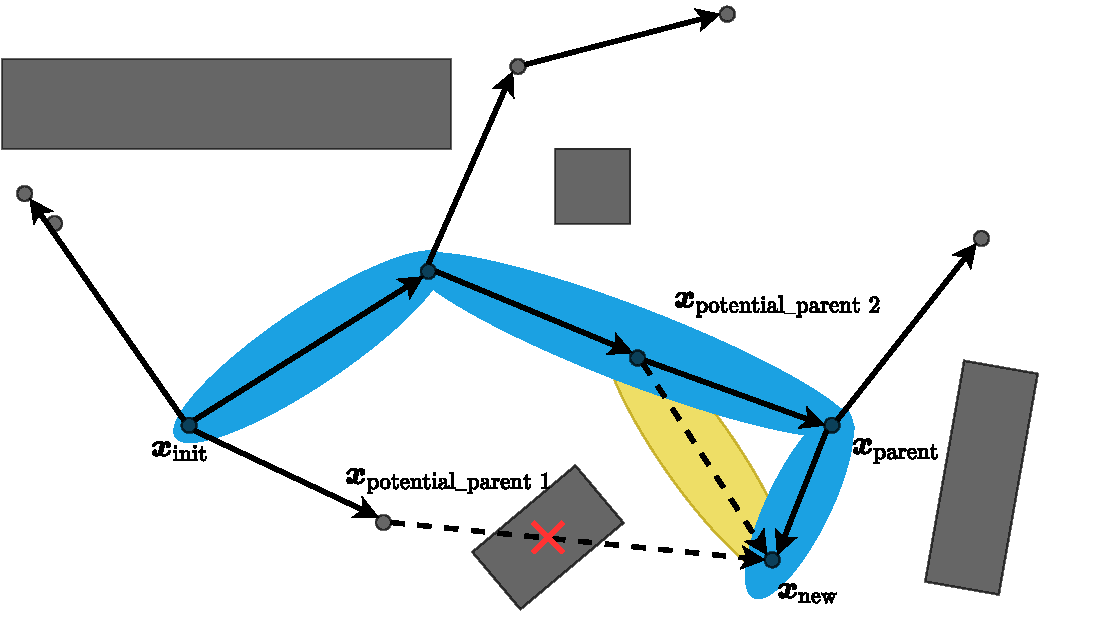
\includegraphics[width=0.8\textwidth]{images/choose_parent.pdf}
    \caption{寻找母节点进行拓展流程}
    \label{fig:寻找母节点进行拓展流程}
\end{figure}

在拓展完成后再以该点作为中间点,寻找是否存在一个树节点,使得根节点到新拓展的节点再到该树节点的航程,比根节点到该树节点的原本的航程要小,是则对该节点的连接方式进行调整,使起航迹的上一个节点为新拓展的节点,如图~\ref{fig:Rewire重布线流程}所示,在将采样点\( \boldsymbol{x}_{\textrm{new}} \)拓展入随机树后,存在着\( \boldsymbol{x}_{\textrm{potential\_child 1}} \)、\( \boldsymbol{x}_{\textrm{potential\_child 2}} \)以及\( \boldsymbol{x}_{\textrm{potential\_child 3}} \)三点潜在的子节点,但由于\( \boldsymbol{x}_{\textrm{init}} \to \boldsymbol{x}_{\textrm{new}} \to \boldsymbol{x}_{\textrm{potential\_child 1}} \)的航程大于\( \boldsymbol{x}_{\textrm{init}} \to \boldsymbol{x}_{\textrm{potential\_child 1}} \)的航程\( \boldsymbol{x}_{\textrm{init}} \to \boldsymbol{x}_{\textrm{new}} \to \boldsymbol{x}_{\textrm{potential\_child 3}} \)的航程大于\( \boldsymbol{x}_{\textrm{init}} \to \boldsymbol{x}_{\textrm{potential\_child 3}} \)的航程,\( \boldsymbol{x}_{\textrm{potential\_child 1}} \)和\( \boldsymbol{x}_{\textrm{potential\_child 3}} \)将不被考虑,而\( \boldsymbol{x}_{\textrm{init}} \to \boldsymbol{x}_{\textrm{new}} \to \boldsymbol{x}_{\textrm{potential\_child 2}} \)的航程小于\( \boldsymbol{x}_{\textrm{init}} \to \boldsymbol{x}_{\textrm{potential\_child 2}} \)的航程,故取消\( \boldsymbol{x}_{\textrm{potential\_child 2}} \)与\( \boldsymbol{x}_{\textrm{potential\_child 3}} \)的连接,新增\( \boldsymbol{x}_{\textrm{potential\_child 2}} \)与\( \boldsymbol{x}_{\textrm{new}} \)的连接,该机制为RRT-Connect算法的Rewire重布线机制。

\begin{figure}[!htbp]
    \centering
    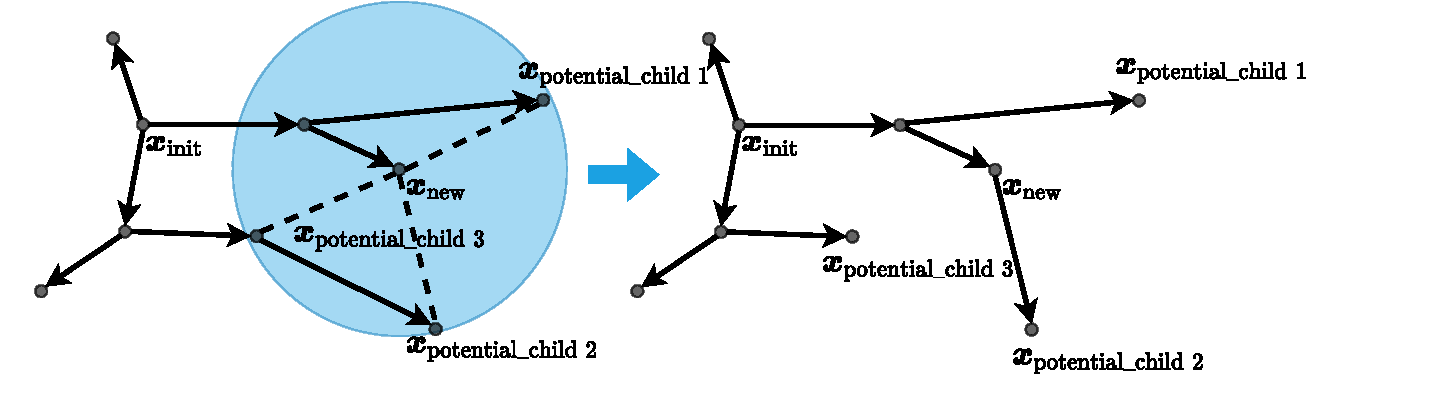
\includegraphics[width=\textwidth]{images/rewire.pdf}
    \caption{Rewire重布线流程}
    \label{fig:Rewire重布线流程}
\end{figure}

该函数的伪代码如算法~\ref{alg:extend_function}所示,为便于算法~\ref{alg:rrt*-connect}中判断采样点是否拓展入随机树成功,以便于接下来对随机树进行连接、合并等操作,故Extend函数需要将是否拓展如随机树成功的结果进行返回至上一层函数。

\begin{algorithm}[!htbp]
  \caption{Extend函数} % 名称
  \label{alg:extend_function}
  \begin{algorithmic}[1]
    \REQUIRE 
        \( \tau \):随机树;
        \( \boldsymbol{x}_{\textrm{new}} \):采样点;
        \( \boldsymbol{x}_{\textrm{near}} \):最近点。
    \ENSURE 
        \( S \):采样点拓展进随机树中是否成功。
    \IF{\( \textrm{CollisionFree}(\boldsymbol{x}_{\textrm{new}}) \)}
        \STATE \(\mathcal{X}_\textrm{near} \gets \textrm{NearC}(\tau, \boldsymbol{x}_{\textrm{new}}) \);
        \STATE \( \boldsymbol{x}_{\textrm{min}} \gets \textrm{ChooseParent}(\mathcal{X}_{\textrm{near}}, \boldsymbol{x}_{\textrm{near}}, \boldsymbol{x}_{\textrm{new}}) \);
        \STATE \( \tau.\textrm{addNodeEdge}(\boldsymbol{x}_{\textrm{min}}, \boldsymbol{x}_{\textrm{new}}) \);
        \STATE \( \tau.\textrm{rewire}() \);
        \RETURN \TRUE;
    \ENDIF
    \RETURN \FALSE;
  \end{algorithmic}
\end{algorithm}

\subsection{基于A*的动态场景下的无人机航迹规划算法设计}

动态场景下的无人机航迹规划算法,是用于为单体无人机提供应对可能存在突发事况的动态环境下的措施。该算法根据已有的地图信息和配备的传感器探测到的障碍物信息,对由服务器为其规划的路径进行修订,保障其飞行的安全性与稳定性,并确保能够及时到达任务地点。由于该算法是在无人机飞行过程中运行的,需要实时对飞行航迹进行修改,因此该算法对运行时间有着较高的要求。

\subsubsection{算法设计}

同样根据\citet{braun2019ComparisonRRTAlgorithmsa}的研究结果,在大小较大且精度较低或大小较小且精度较高的地图信息中寻找最短路径,使用A*及其派生算法得到的路径不论是从稳定性还是从运算速度上看,都远远好于RRT及其派生算法。而在单无人机的实时避障算法中,由于其对航迹修订的范围仅为无人机传感器能够感知的范围,属于精度较高但地图大小较小的类型,因此适用A*算法来解决该问题。

A*算法最初由\citet{hart1968FormalBasisHeuristica}提出,是将启发式的方法如BFS等,应用于常规的方法如Dijkstra算法等的一种算法。该算法通过逐步对每一个节点\( n \)进行从起点经过该点再至目标点的估计代价或距离,来不断更新优化,最终得到地图信息中从起点到目标点的最短路径,其距离的估计函数用公式表达为:

\begin{equation}
    f(n) = g(n) + h(n) \nonumber
\end{equation}

其中,\( f(n) \)为对于节点\( n \),从起点经过该点再至目标点的估计代价或距离;\( g(n) \)为从起点至节点\( n \)的实际距离;\( h(n) \)为从节点\( n \)至目标点的估计距离,通常用欧式距离,即\( d(\boldsymbol{x}_n, \boldsymbol{x}_0) = \parallel \boldsymbol{x}_n - \boldsymbol{x}_0 \parallel ^ 2\),进行估计。

A*算法的流程的伪代码如算法~\ref{alg:A-Star}所示。

\begin{algorithm}[!htbp]
  \caption{A*算法} % 名称
  \label{alg:A-Star}
  \begin{algorithmic}[1]
    \REQUIRE
      $M$: 地图信息;
      $S$: 起点信息;
      $D$: 目标点信息;
    \ENSURE
      $P$: 飞行航迹;
    \STATE 初始化集合 \( L \gets \text{init}(S)\);
    \WHILE {\( ! \text{L.isEmpty}() \)}
        \STATE 估计距离最小的节点 \( p_\textrm{min\_fn} \gets \textrm{FindMin}(L) \);
        \IF{\( p_\textrm{min\_fn} == D \)}
            \STATE \( P \gets \textrm{GetTrajectory}(p_{\textrm{min\_fn}}) \);
            \STATE break;
        \ENDIF
        \STATE 获取四周尚未搜索过的节点 \( p_\textrm{unexplored} \gets \text{FindNew} (p_{\textrm{min\_fn}}) \);
        \FORALL{\( p_{\textrm{cur}} \) in \(p_\textrm{unexplored}\)}
            \IF {\( \text{IsBlockedByEnv}(p_{\textrm{cur}}) \)}
                \STATE continue;
            \ENDIF
            \STATE 将可行节点添加入集合中 \( \text{L.add}(p_{\textrm{cur}})\);
        \ENDFOR
    \ENDWHILE
    \RETURN \( P \);
  \end{algorithmic}
\end{algorithm}

\subsubsection{算法应用流程}

以图~\ref{fig:单无人机避障实际场景示例}为例,假设实际场景中的障碍物如图~\ref{fig:单无人机避障实际场景示例}中的分布,此时无人机以到达图中的位置,继续沿着原定的飞行航迹前往目标点,而原本为该无人机规划的飞行航迹和已知的地图信息则如图~\ref{fig:单无人机避障规划示例}所示。很明显,已知的地图信息与实际信息存在可能在精细度上的差异,缺失了在飞行航迹中存在的障碍物,导致若无人机按照原本规划的飞行航迹不进行修订,则该无人机将会与障碍物发生碰撞从而造成无人机损毁及侦察任务的无法完成。

\begin{figure}[!htbp]
    \centering
    \begin{subfigure}[t]{0.48\textwidth}
        \captionsetup{justification=centering}
        \begin{minipage}[b]{\linewidth}
            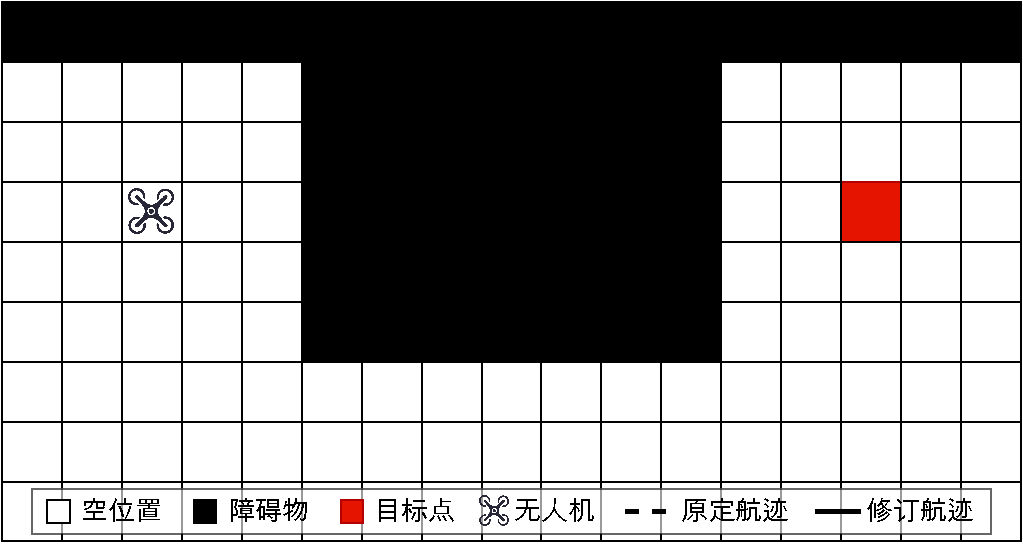
\includegraphics[width=\textwidth]{images/单无人机避障实际场景示例.pdf}
            \caption{单无人机避障实际场景示例}
            \label{fig:单无人机避障实际场景示例}
        \end{minipage}
    \end{subfigure}
    \begin{subfigure}[t]{0.48\textwidth}
        \captionsetup{justification=centering}
        \begin{minipage}[b]{\linewidth}
            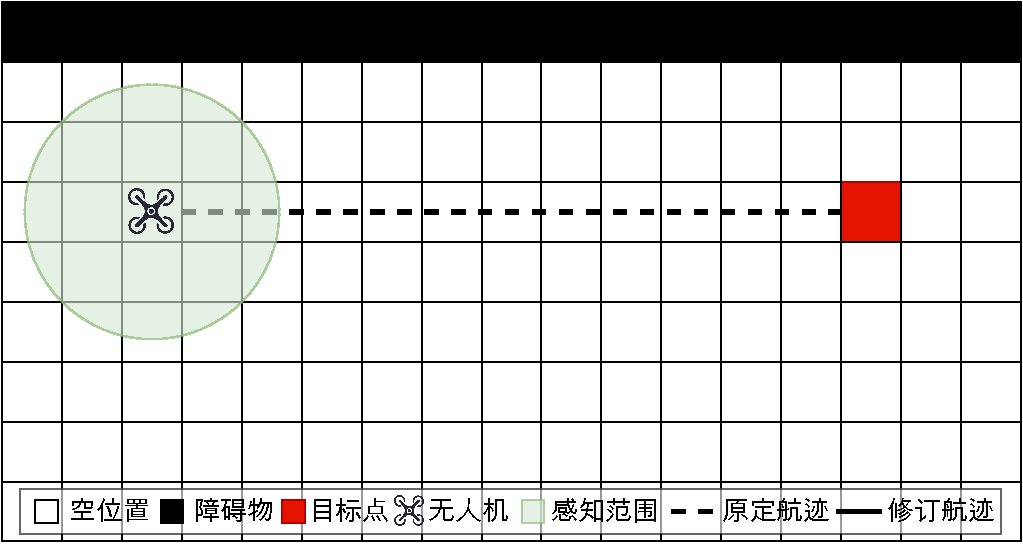
\includegraphics[width=\textwidth]{images/单无人机避障规划场景示例.pdf}
            \caption{单无人机避障规划示例}
            \label{fig:单无人机避障规划示例}
        \end{minipage}
    \end{subfigure}
    \caption{单无人机避障示例}
    \label{fig:单无人机避障示例}
\end{figure}

此时,该无人机可以根据其自身携带的能够探测障碍物的传感器设备,如成本高昂但精度与探测范围都很高的激光雷达、成本低廉但精度及探测范围较差的超声波探测器等,通过不断地对已有的地图信息进行修正,并运行A*算法来修订原有航迹,最终平安无事地到达任务点执行侦察任务。以图~\ref{fig:单无人机避障示例}中的情景为例,无人机在按照原有航迹进行飞行前行时,传感器探测到前方存在障碍物,此时运行A*算法进行航迹的修订,之后按照修订后的航迹进行飞行,如图~\ref{fig:单无人机第一次修订航迹进行避障}所示;但此时无人机所存储的地图信息明显与图~\ref{fig:单无人机避障实际场景示例}中不同,按新的航迹前行仍然会障碍物相撞,因此在无人机继续前行时,依然检测到了与航迹存在冲突的障碍物,此时需再运行A*算法,进一步修订飞行航迹,如图~\ref{fig:单无人机第二次修订航迹进行避障}所示;在完成对障碍物正面的绕行后,无人机继续检测到了与航迹冲突的障碍物,再一次运行了A*算法对航迹进行修订,如图~\ref{fig:单无人机第三次修订航迹进行避障}所示;不断重复以上过程,如图~\ref{fig:单无人机第四次修订航迹进行避障}、图~\ref{fig:单无人机第五次修订航迹进行避障}和图~\ref{fig:单无人机第六次修订航迹进行避障}所示,直至无人机能够顺利沿着修订航迹到达任务点的位置。

\begin{figure}[!htbp]
    \centering
    \begin{subfigure}[t]{0.48\textwidth}
        \captionsetup{justification=centering}
        \begin{minipage}[b]{\linewidth}
            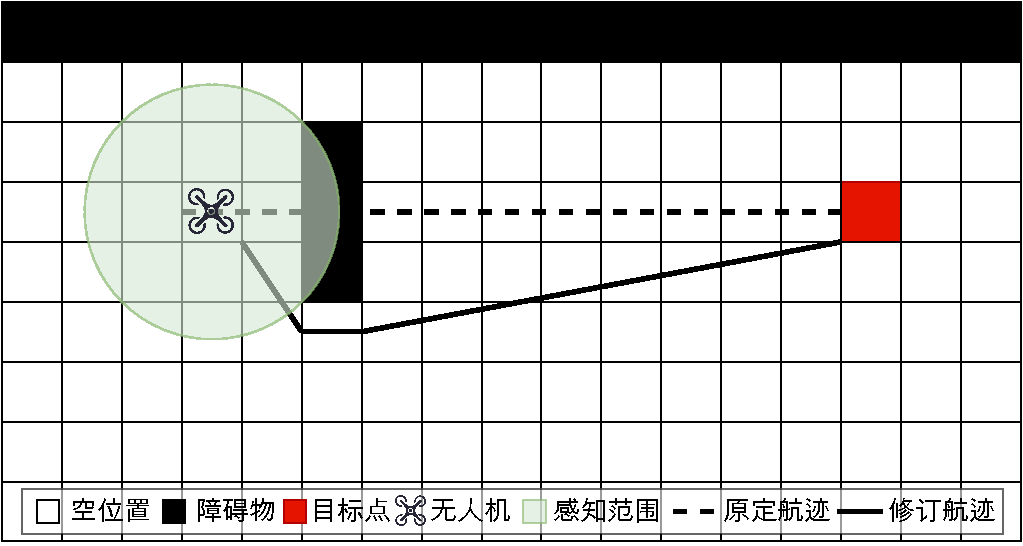
\includegraphics[width=\textwidth]{images/单无人机避障步骤示例1.pdf}
            \caption{无人机第一次修订航迹进行避障}
            \label{fig:单无人机第一次修订航迹进行避障}
        \end{minipage}
    \end{subfigure}
    \begin{subfigure}[t]{0.48\textwidth}
        \captionsetup{justification=centering}
        \begin{minipage}[b]{\linewidth}
            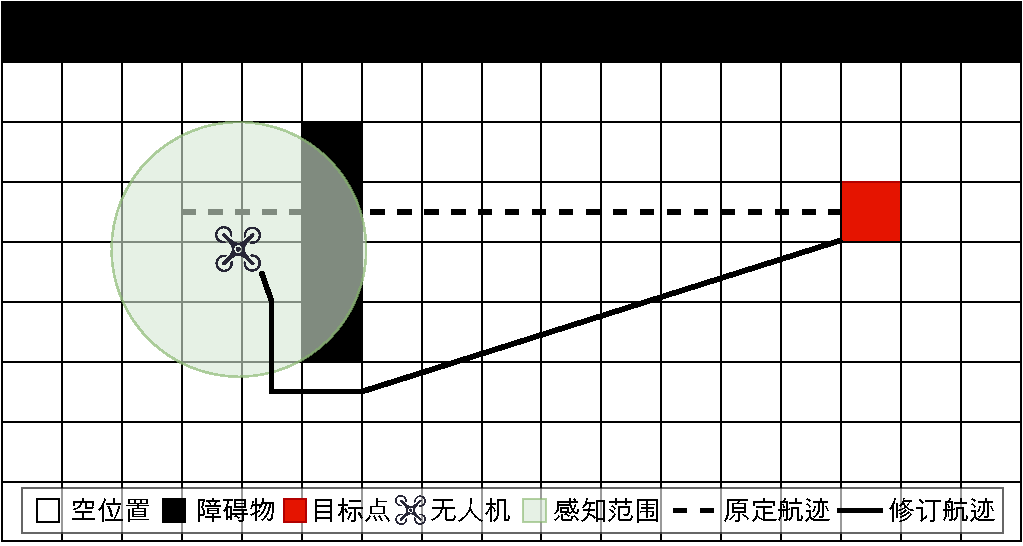
\includegraphics[width=\textwidth]{images/单无人机避障步骤示例2.pdf}
            \caption{无人机第二次修订航迹进行避障}
            \label{fig:单无人机第二次修订航迹进行避障}
        \end{minipage}
    \end{subfigure}
    \begin{subfigure}[t]{0.48\textwidth}
        \captionsetup{justification=centering}
        \begin{minipage}[b]{\linewidth}
            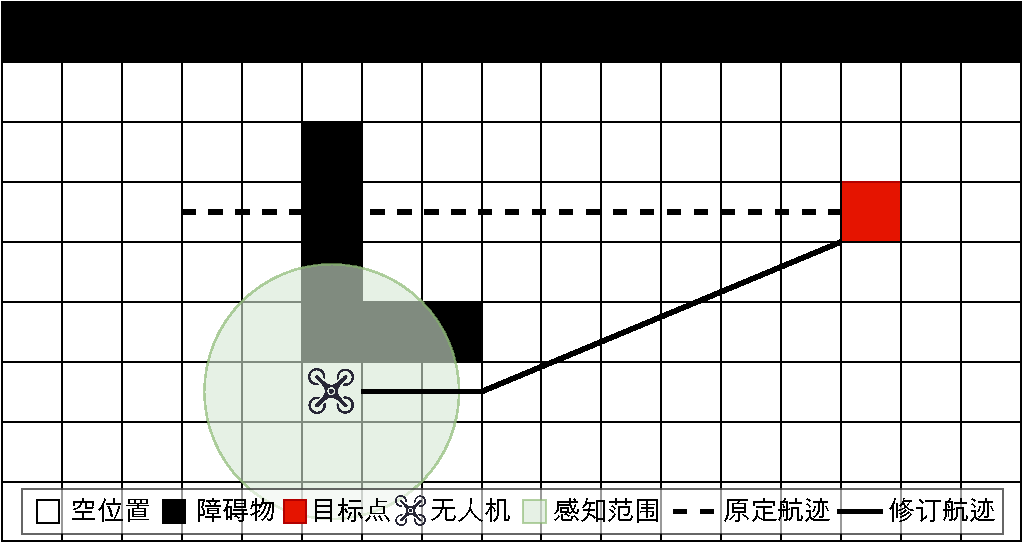
\includegraphics[width=\textwidth]{images/单无人机避障步骤示例3.pdf}
            \caption{无人机第三次修订航迹进行避障}
            \label{fig:单无人机第三次修订航迹进行避障}
        \end{minipage}
    \end{subfigure}
    \begin{subfigure}[t]{0.48\textwidth}
        \captionsetup{justification=centering}
        \begin{minipage}[b]{\linewidth}
            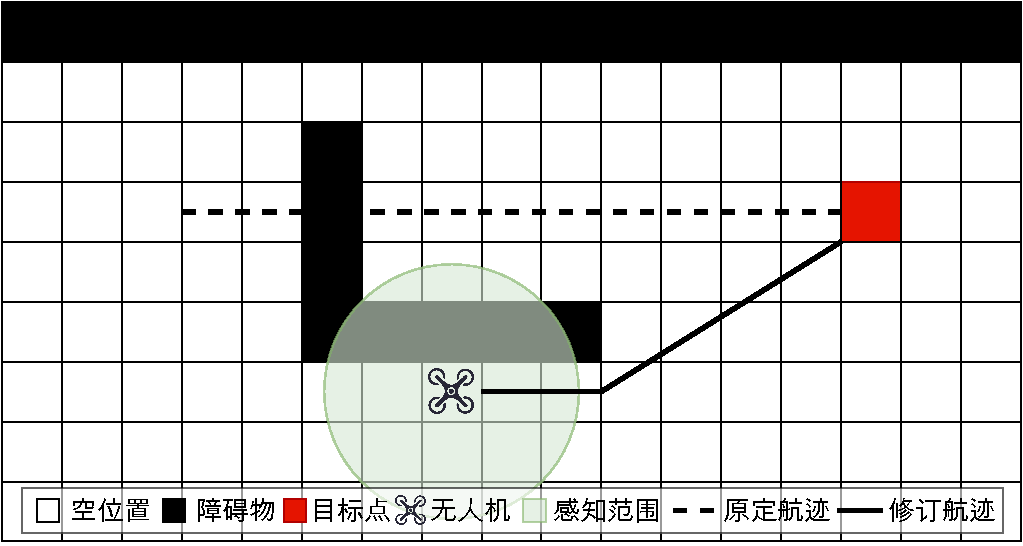
\includegraphics[width=\textwidth]{images/单无人机避障步骤示例4.pdf}
            \caption{无人机第四次修订航迹进行避障}
            \label{fig:单无人机第四次修订航迹进行避障}
        \end{minipage}
    \end{subfigure}
    \begin{subfigure}[t]{0.48\textwidth}
        \captionsetup{justification=centering}
        \begin{minipage}[b]{\linewidth}
            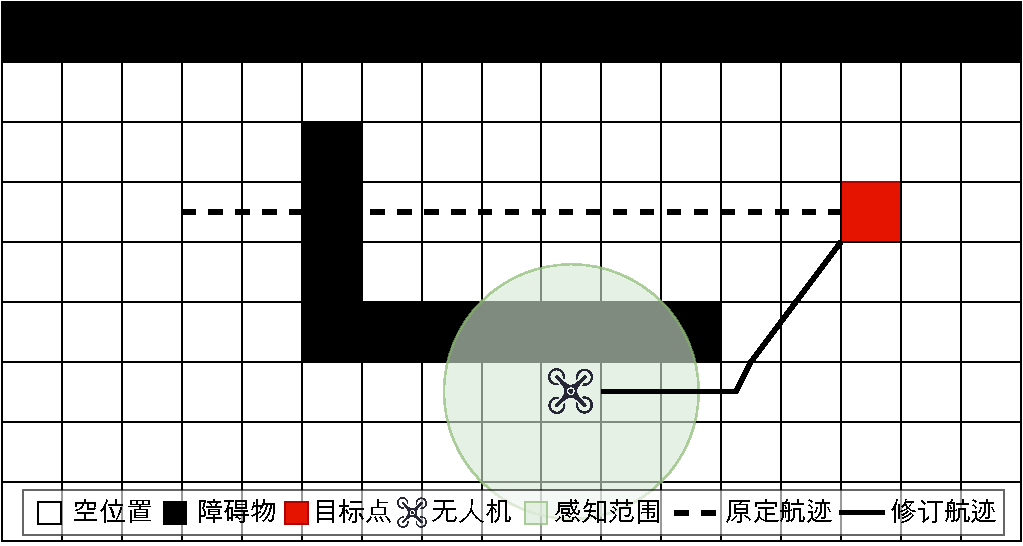
\includegraphics[width=\textwidth]{images/单无人机避障步骤示例5.pdf}
            \caption{无人机第五次修订航迹进行避障}
            \label{fig:单无人机第五次修订航迹进行避障}
        \end{minipage}
    \end{subfigure}
    \begin{subfigure}[t]{0.48\textwidth}
        \captionsetup{justification=centering}
        \begin{minipage}[b]{\linewidth}
            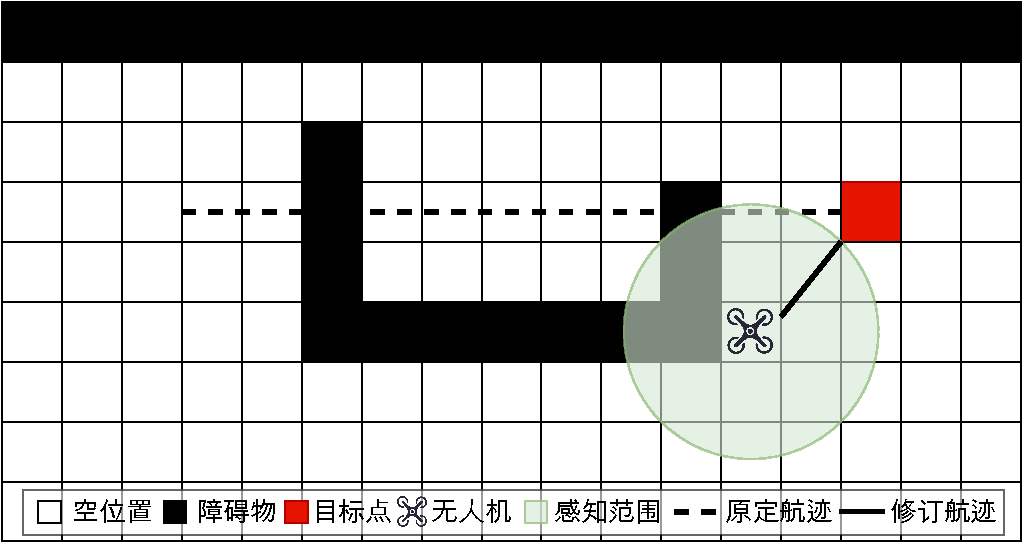
\includegraphics[width=\textwidth]{images/单无人机避障步骤示例6.pdf}
            \caption{无人机第六次修订航迹进行避障}
            \label{fig:单无人机第六次修订航迹进行避障}
        \end{minipage}
    \end{subfigure}
    \caption{无人机实时修订航迹进行避障}
    \label{fig:单无人机实时修订航迹进行避障}
\end{figure}

\subsubsection{算法流程图}

根据上述内容,本文提出的单无人机下的实时避障算法的运行流程如下,在无人机收到指令后或完成上一任务点的收集型侦察任务后,由无人机的飞行控制系统控制无人机按照所给飞行航迹进行飞行,并在飞行过程中不断地根据障碍物探测传感器的结果更新其地图数据库储存的地图信息,根据该地图信息来判断当前无人机的飞行航迹是否与已探测到的障碍物存在冲突,若存在冲突,则调用A*算法,先计算当前无人机与航迹点的估计距离,再更新周围点的估计距离,之后不断更新已知点中估计距离最小的点的周围点的估计距离,直到到达目标点,此时根据得到的修订航迹对原有飞行航迹进行修订,直到到达当前任务点开始执行收集型侦察任务。总流程如图~\ref{fig:单无人机避障算法流程图}所示。

\begin{figure}[!htbp]
    \centering
    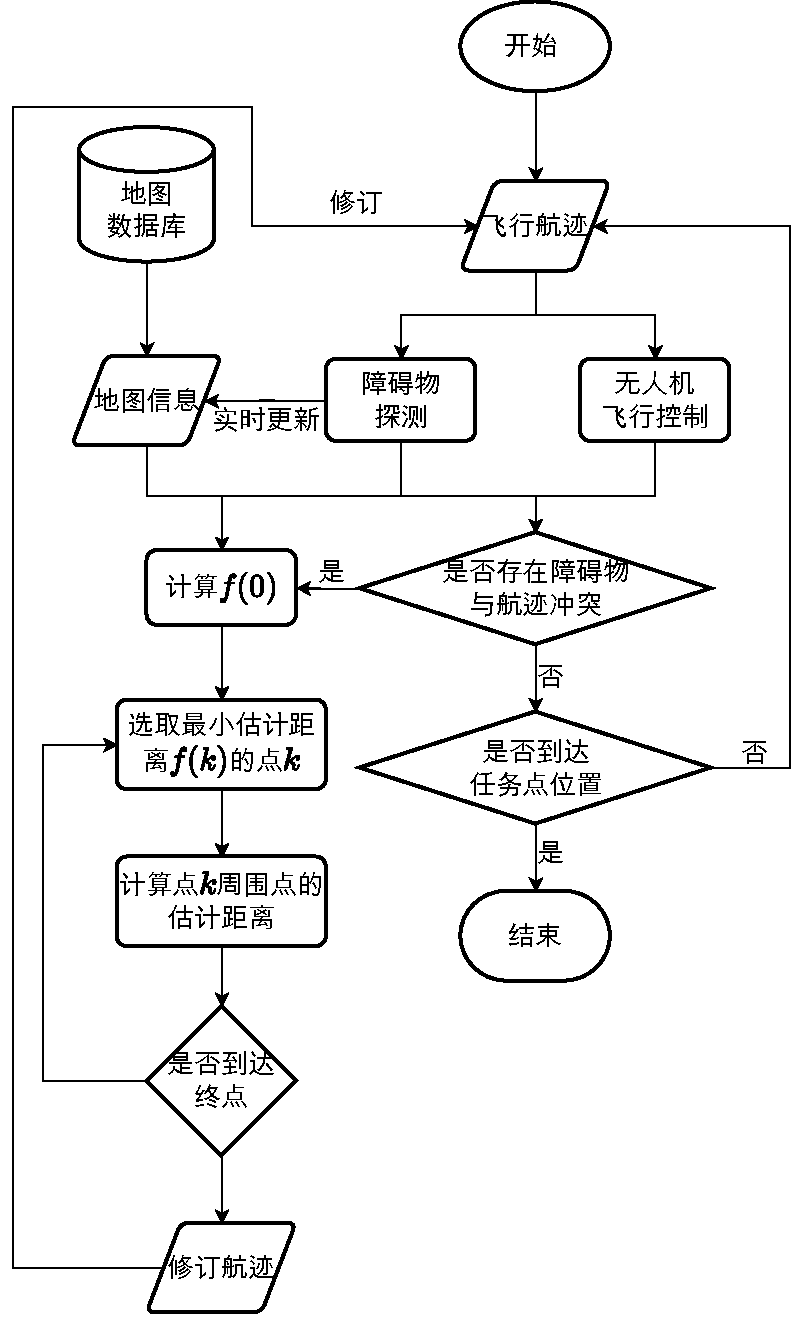
\includegraphics[width=0.7\textwidth]{images/单无人机避障算法总流程图.pdf}
    \caption{单无人机避障算法流程图}
    \label{fig:单无人机避障算法流程图}
\end{figure}


%!TEX root = ../../csuthesis_main.tex

\subsection{基于TSAVN的多无人机任务调度分配算法设计} \label{sec:TSAVN}

K-Means算法是一种机器学习中常用的聚类算法,其认为样本间距离越近,则这两个样本的相似性越大。其时间复杂度仅为\(tknm\),其中\(t\)为迭代次数,\(k\)为类别簇的个数,\(n\)为样本个数,\(m\)为样本的纬度,能够在很短时间内将\(n\)个样本根据欧式距离计算样本间的相似度,无需对样本进行任何标注,即可将其聚类分为\(k\)个类别。

模拟退火算法(Simulated Annealing Algorithm, SA)是一种模拟热力学中退火的过程,从某一较高的初始温度开始,随着算法迭代次数的增加而逐渐降低温度,结合概率跳跃的特性使得算法在温度高时具备跳出当前所在的局部最优解,在解的邻域结构中随机搜索全局最优解的启发式算法。

变邻域搜索算法(Varied Neighborhood Search Algorithm, VNS)是一种改进型的局部搜索算法,其利用了全局最优解必然在任意邻域结构中仍为局部最优解的特点,利用不同邻域动作所构成的邻域结构进行交替搜索,拓展了解的搜索范围,在集中性与疏散性之间达到了较好的平衡。

\subsubsection{算法设计} 

多无人机任务调度分配算法将分为两个阶段,分别是对任务进行预分配的预分配阶段,以及基于预分配的任务信息,得到无人机所需数量及各无人机的任务有序序列的再分配阶段,如图~\ref{fig:多无人机任务调度分配阶段示意图}所示,其中,在任务预分配阶段,由于对于无人机而言,若执行相邻任务距离较远,且跨过了数个其他任务点,那么其最终的航程通常较大,而执行相邻任务距离较远,且中途没有其他任务点,那么其最终的航程通常较小,因此可以通过对任务点间的飞行航迹的航程进行聚类来得到初步的任务预分配结果,是合理的;之后,由于任务预分配结果仅仅只是根据航程信息对任务进行聚类操作,不具备问题所需的无人机数量、各无人机所要执行的任务有序序列,因此在任务再分配阶段,本文提出了TSAVN算法,其流程图如图~\ref{fig:多无人机任务调度分配阶段示意图}所示。

\begin{figure}[!htbp]
    \centering
    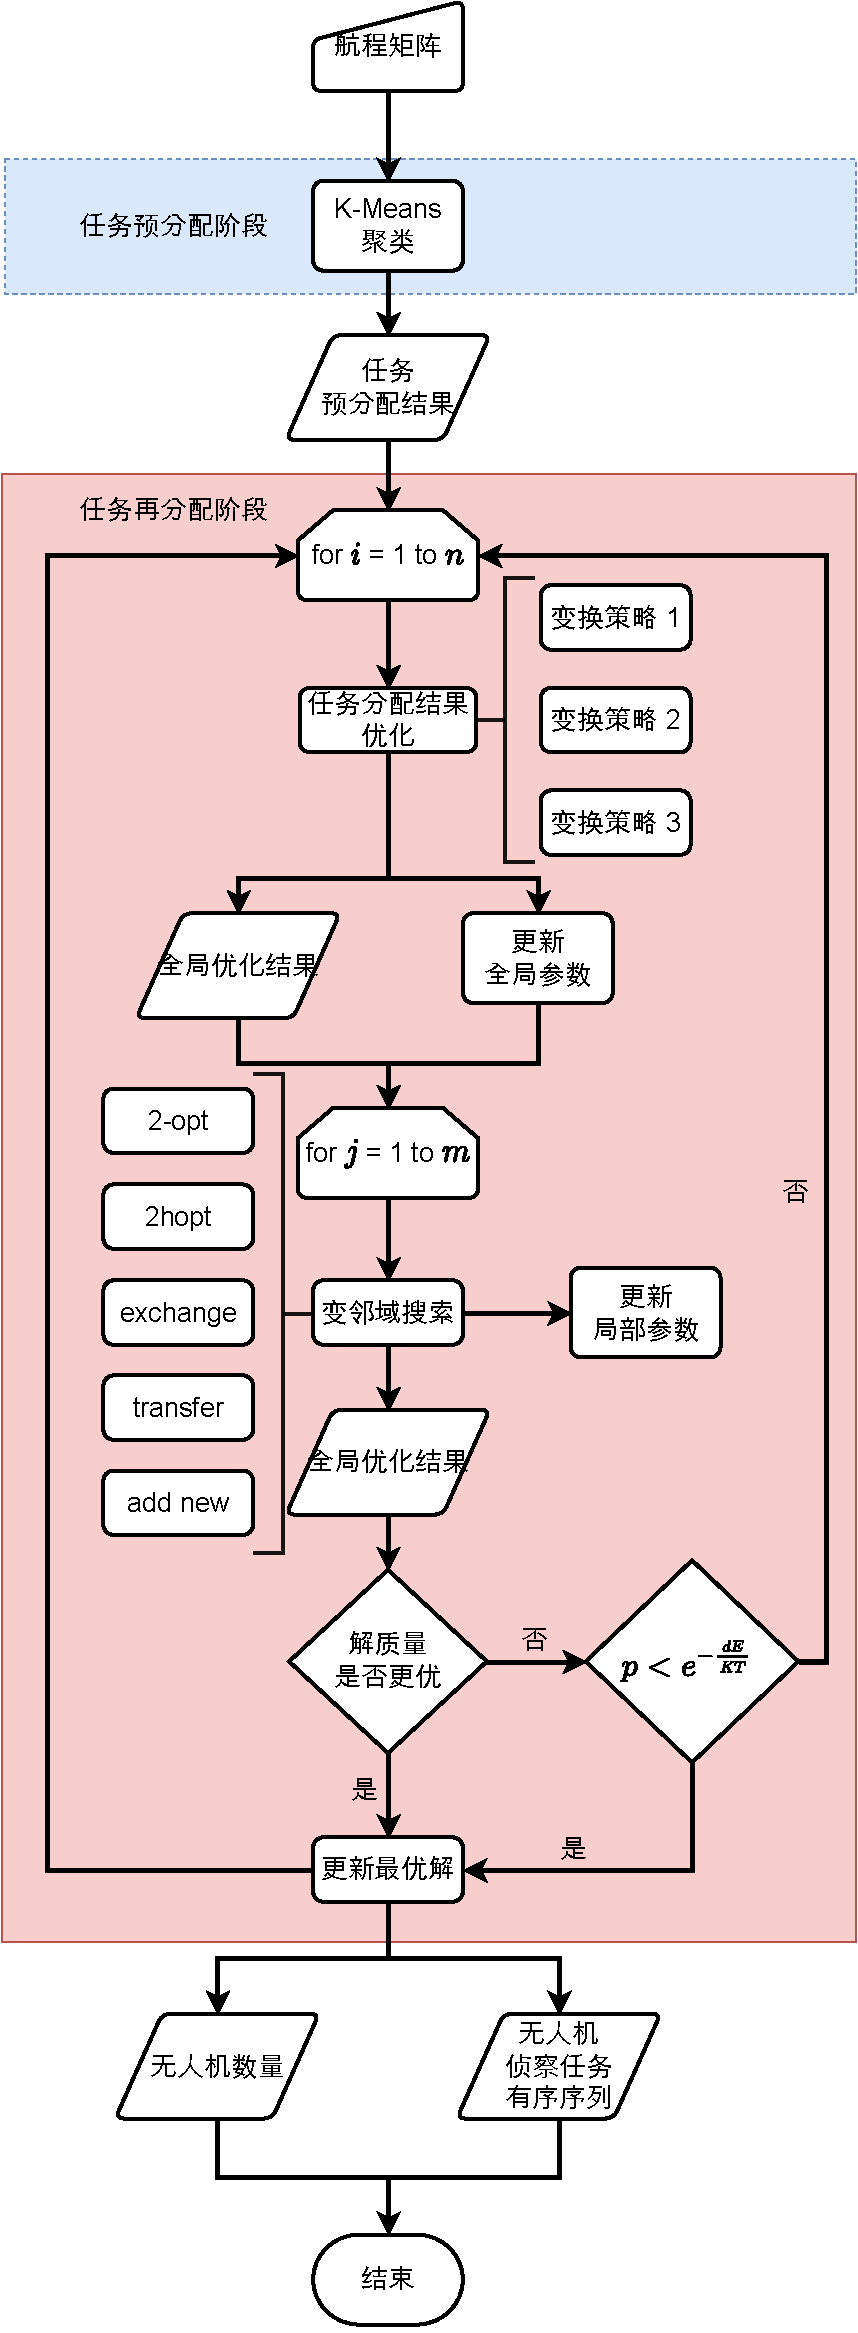
\includegraphics[width=0.55\textwidth]{images/多无人机任务调度分配阶段示意图.pdf}
    \caption{多无人机任务调度分配阶段示意图}
    \label{fig:多无人机任务调度分配阶段示意图}
\end{figure}

由于直接使用任务点数据会导致解空间过大的问题,故先使用K-Means算法根据点间的航程数据,对任务点数据进行聚类,使得各个类内距离尽可能近,类间距离尽可能远,实现任务的预分配,从而能够有效地降低各个部分的解空间,便于并行、高效地运行算法。

本小节以最小化航迹距离作为聚类依据,自下而上对各任务点进行聚类。同时为尽可能保证同一个簇里航迹之和最小,在聚类完成后,将结果放入局部优化器中生成各个簇中最优的车辆安排、配置及路径等数据,即初始解生成。

初始解生成的伪代码如算法\ref{alg:Solution Initialization}所示:

\begin{algorithm}[!htbp]
  \caption{初始解生成器} % 名称
  \label{alg:Solution Initialization}
  \begin{algorithmic}[1]
    \REQUIRE 
      \( V \): 无人机起飞点与任务点的点集;
      \( M \): 所有任务点的任务数据集;
      \( C \): 所有车型数据集;
    \ENSURE 
      \( S \): 初始解;
    \STATE 初始化类簇标签 \( L \);
    \REPEAT
        \STATE 获取距离矩阵 \(D \gets \textrm{CalcDistanceMatrix}(V, L) \);
        \STATE 获取所有拥有最小距离的两个簇的组合 \(C \gets \textrm{FindMinDisCombs}(L, D) \);
        \FOR{\( i, j \in C \)}
            \IF{\( \textrm{not} \textrm{ReachCriteria}(i, j, L) \)}
                \STATE 更新标签 \( L \gets \textrm{merge}(i, j, L) \);
            \ENDIF
        \ENDFOR
    \UNTIL {\( \textrm{AllReachCriteria}(L) \)}
    \STATE \( S \gets \textrm{PartialSolver}(L, V, M, C) \);
  \end{algorithmic}
\end{algorithm}

为了增加算法收敛至全局最优解的概率,以及尽可能避免算法生成的解质量较差的情况发生,本小节选取了3种不同的解的变化策略,以及5种基于这3种方式的邻域结构来对全局解中不同任务簇的分类进行一定的调整。

第一种变化策略为任务点的转移,将一个簇中的任务点转移至另一个簇中,过程如图\ref{fig:conversion_way_1}所示。基于该变化策略,本文提出了两种随机性不同的邻域结构。一种在两个簇中的选取及待转移的任务点的选取中全部依赖随机,即随机性较高,其动作过程的伪代码如算法\ref{alg:Stochastic Transfer Neighborhood Structure}所示;另一种则随机选取一个簇并随机选取簇中的一个任务点,将其转移至离该簇最近的另一个簇中,随机性相对于前者更低,但相应的计算时间更多,其动作过程的伪代码如算法\ref{alg:Proximity Transfer Neighborhood Structure}所示。

\begin{figure}[!htbp]
    \centering
    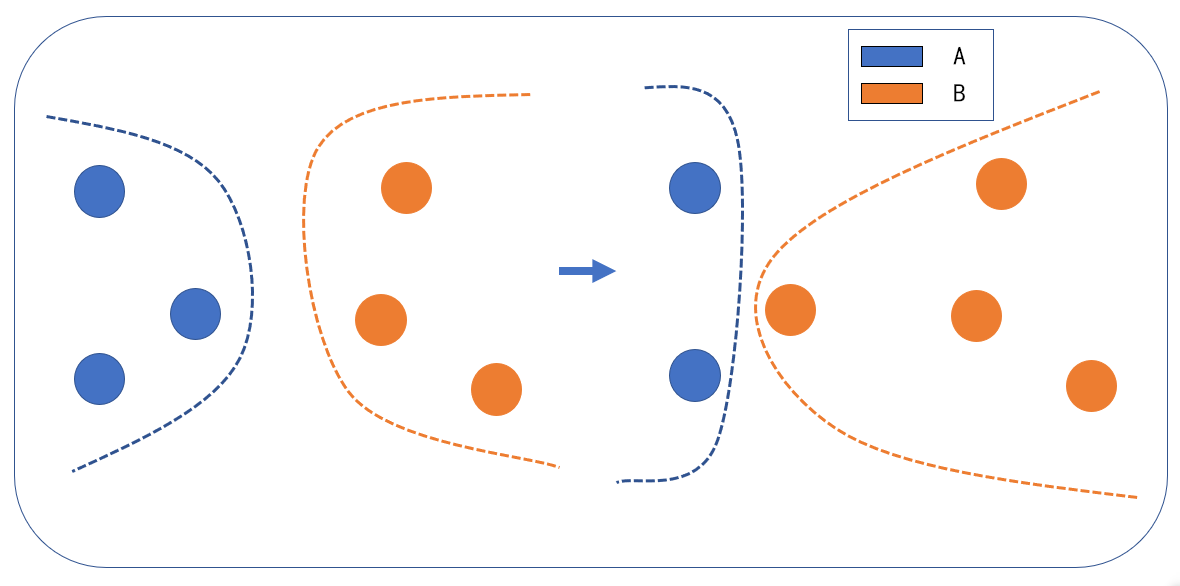
\includegraphics[width=0.7\textwidth]{images/全局邻域1_en.png}
    \caption{变化策略 1}
    \label{fig:conversion_way_1}
\end{figure}

\begin{algorithm}[!htbp]
  \caption{随机转移算子} % 名称
  \label{alg:Stochastic Transfer Neighborhood Structure}
  \begin{algorithmic}[1]
    \REQUIRE
      $V$: 无人机起飞点与任务点的点集;
      $L$: 先前的类簇标签;
    \ENSURE
      $L^*$: 新的类簇标签;
    \STATE 随机寻找两个类簇 $\ell_1, \ell_2 \gets$ FindTwoDifferentLabel($L$);
    \STATE 在类簇$\ell_1$中寻找一个随机的任务点$v_1$;
    \STATE 更新任务点 $v_1$'的标签从 $\ell_1$ 变为 $\ell_2$;
    \STATE $L^* \gets L$;
  \end{algorithmic}
\end{algorithm}

\begin{algorithm}[!htbp]
  \caption{就近转移算子} % 名称
  \label{alg:Proximity Transfer Neighborhood Structure}
  \begin{algorithmic}[1]
    \REQUIRE
      $V$: 无人机起飞点与任务点的点集;
      $L$: 先前的类簇标签;
    \ENSURE
      $L^*$: 新的类簇标签;
    \STATE 随机寻找一个类簇 $\ell_1 \gets$ FindLabel($L$);
    \STATE 寻找一个距离$\ell_1$最近的类簇 $\ell_2 \gets$ FindNearestLabel($L, \ell_1$);
    \STATE 在类簇$\ell_1$中寻找一个随机的任务点$v_1$;
    \STATE 更新任务点 $v_1$'的标签从 $\ell_1$ 变为 $\ell_2$;
    \STATE $L^* \gets L$;
  \end{algorithmic}
\end{algorithm}

第二种变化策略为任务点的交换,在两个不同的簇中各自选择一个任务点进行交换,其过程如算法\ref{fig:conversion_way_2}所示。基于该变化策略,本文提出了两种随机性不同的邻域结构,一种在两个簇的选取及各自的待交换的任务点的选取中全部依赖随机,即随机性较高,其动作过程的伪代码如算法\ref{alg:Stochastic Exchange Neighborhood Structure}所示;另一种则随机选取一个簇,并将离它最近的簇作为另一个簇,分别随机选取簇中的任务点进行交换,随机性相对于前者更低,但相应的计算时间会更多,其动作过程的伪代码如算法\ref{alg:Proximity Exchange Neighborhood Structure}所示。

\begin{figure}[!htbp]
    \centering
    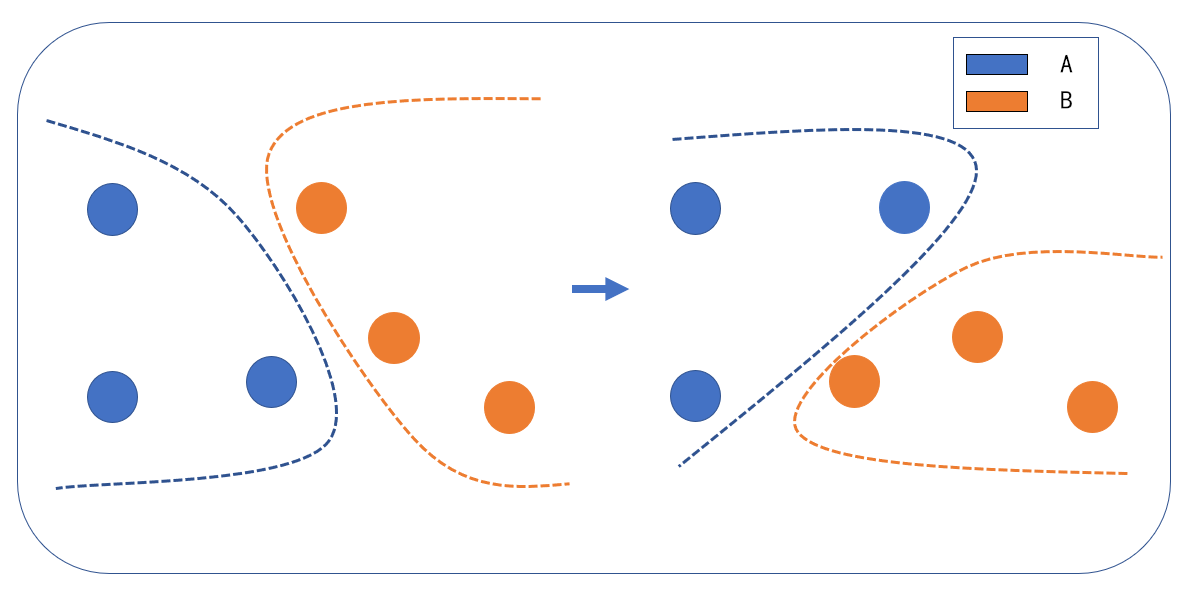
\includegraphics[width=0.7\textwidth]{images/全局邻域2_en.png}
    \caption{变化策略 2}
    \label{fig:conversion_way_2}
\end{figure}

\begin{algorithm}[!htbp]
  \caption{随机交换算子} % 名称
  \label{alg:Stochastic Exchange Neighborhood Structure}
  \begin{algorithmic}[1]
    \REQUIRE
      $V$: 无人机起飞点与任务点的点集;
      $L$: 先前的类簇标签;
    \ENSURE
      $L^*$: 新的类簇标签;
    \STATE 随机寻找两个类簇 $\ell_1, \ell_2 \gets$ FindTwoDifferentLabel($L$);
    \STATE 在类簇$\ell_1$中寻找一个随机的任务点$v_1$;
    \STATE 在类簇$\ell_2$中寻找一个随机的任务点$v_2$;
    \STATE 更新任务点 $v_1$'的标签从 $\ell_1$ 变为 $\ell_2$;
    \STATE 更新任务点 $v_2$'的标签从 $\ell_2$ 变为 $\ell_1$;
    \STATE $L^* \gets L$;
  \end{algorithmic}
\end{algorithm}

\begin{algorithm}[!htbp]
  \caption{就近交换算子} % 名称
  \label{alg:Proximity Exchange Neighborhood Structure}
  \begin{algorithmic}[1]
    \REQUIRE
      $V$: 无人机起飞点与任务点的点集;
      $L$: 先前的类簇标签;
    \ENSURE
      $L^*$: 新的类簇标签;
    \STATE 随机寻找一个类簇 $\ell_1 \gets$ FindLabel($L$);
    \STATE 寻找一个距离$\ell_1$最近的类簇 $\ell_2 \gets$ FindNearestLabel($L, \ell_1$);
    \STATE 在类簇$\ell_1$中寻找一个随机的任务点$v_1$;
    \STATE 在类簇$\ell_2$中寻找一个随机的任务点$v_2$;
    \STATE 更新任务点 $v_1$'的标签从 $\ell_1$ 变为 $\ell_2$;
    \STATE 更新任务点 $v_2$'的标签从 $\ell_2$ 变为 $\ell_1$;
    \STATE $L^* \gets L$;
  \end{algorithmic}
\end{algorithm}

第三种变化策略则是生成新的簇,选取一个任务点作为一个新的类,其过程如算法\ref{fig:Conversion_Way_3}所示。基于该变化策略,本文提出了一种邻域结构,该邻域结构为随机选取一个任务点,若该任务点所属的簇包含的任务点不止该任务点,则将该任务点作为一个新的簇,其动作过程的伪代码如算法\ref{alg:New Cluster Generation Neighborhood Structure}所示;

\begin{figure}[!htbp]
    \centering
    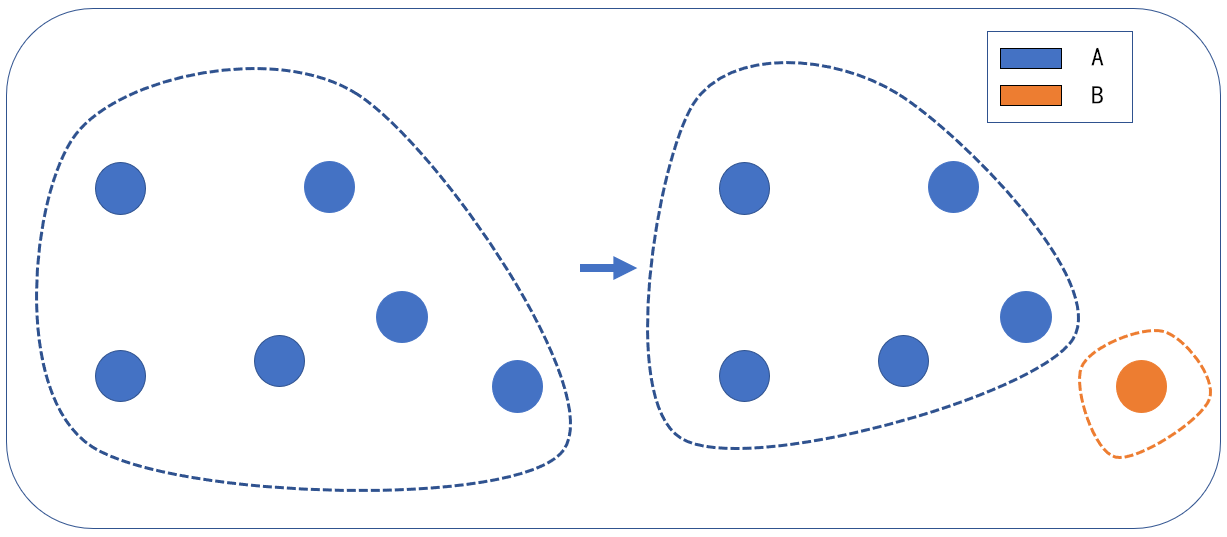
\includegraphics[width=0.7\textwidth]{images/全局邻域3_en.png}
    \caption{变化策略 3}
    \label{fig:Conversion_Way_3}
\end{figure}

\begin{algorithm}[!htbp]
  \caption{新簇生成算子} % 名称
  \label{alg:New Cluster Generation Neighborhood Structure}
  \begin{algorithmic}[1]
    \REQUIRE
      $V$: 无人机起飞点与任务点的点集;
      $L$: 先前的类簇标签;
    \ENSURE
      $L^*$: 新的类簇标签;
    \STATE 随机寻找一个类簇 $\ell_1 \gets$ FindLabel($L$);
    \STATE 在类簇$\ell_1$中寻找一个随机的任务点$v_1$;
    \STATE 设置 $v_1$'的类簇标签为一个新的标签;
    \STATE $L^* \gets L$;
  \end{algorithmic}
\end{algorithm}

为了能够在每一个任务类簇中得到最优解,以获得全局的最优解,同时避免每个任务类簇中发生得到质量较差的解的情况,本小节选取了5种不同的邻域结构来对无人机的侦察任务执行序列进行调整和优化。

第一种邻域结构为2-opt方法\citep{croes1958MethodSolvingTravelingSalesman},如图~\ref{fig:2-opt邻域结构}所示。2-opt方法是选取两任务点\( i \)和\( k \),将\( i \)之前的任务序列保持不变,将\( k \)之后的任务序列保持不变,将\( i \)、\( k \)及其中间的任务的顺序进行翻转,来得到新的任务序列。

\begin{figure}[!htbp]
    \centering
    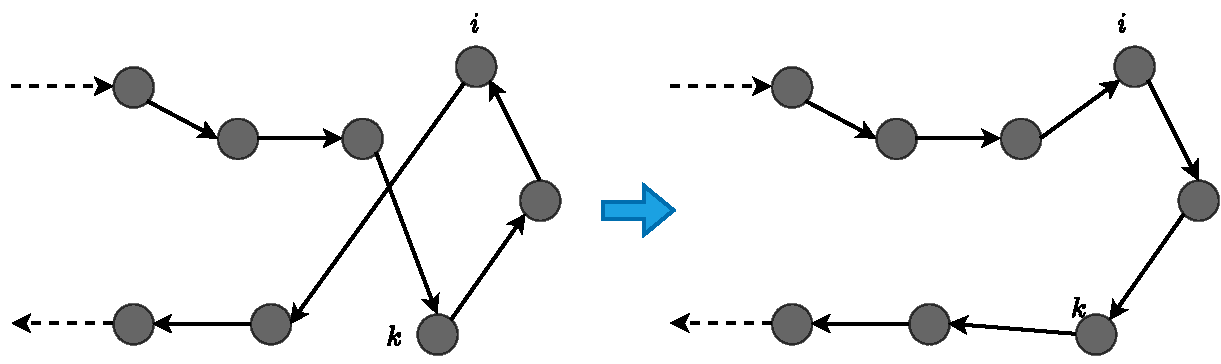
\includegraphics[width=0.8\textwidth]{images/2-opt.pdf}
    \caption{2-opt邻域结构}
    \label{fig:2-opt邻域结构}
\end{figure}

第二种邻域结构为2hopt方法,如图~\ref{fig:2hopt邻域结构}所示。2hopt方法是选取两任务点\( i \)和\( k \),将\( i \)之前的任务序列保持不变,将\( i \)与\( k \)之间的任务保持不变,将\( k \)之后的任务序列保持不变,仅将任务\( i \)、\( k \)进行交换,来得到新的任务序列。

\begin{figure}[!htbp]
    \centering
    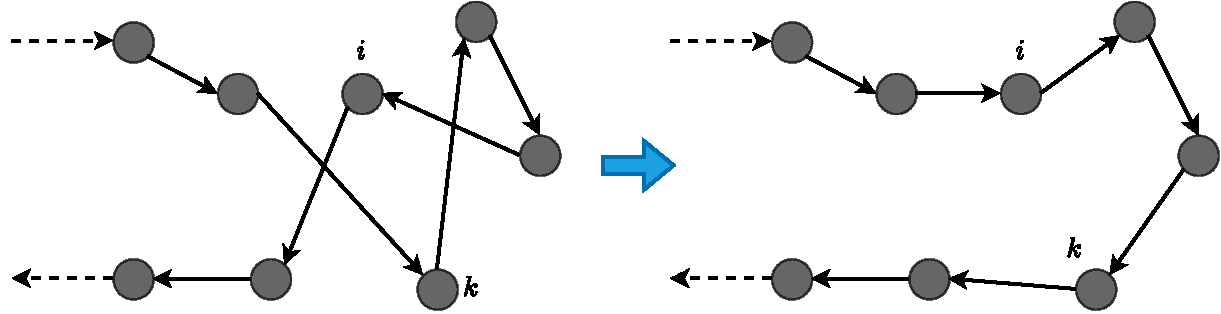
\includegraphics[width=0.8\textwidth]{images/2hopt.pdf}
    \caption{2hopt邻域结构}
    \label{fig:2hopt邻域结构}
\end{figure}

第三种邻域结构为exchange方法,如图~\ref{fig:exchange邻域结构}所示。exchange方法是对于两个无人机的任务序列而言,各选择其中的一个任务点\( i \)和\( k \),将任务点\( i \)和任务点\( k \)进行交换,其余任务点及序列保持不变,以此来得到两条新的任务序列。

\begin{figure}[!htbp]
    \centering
    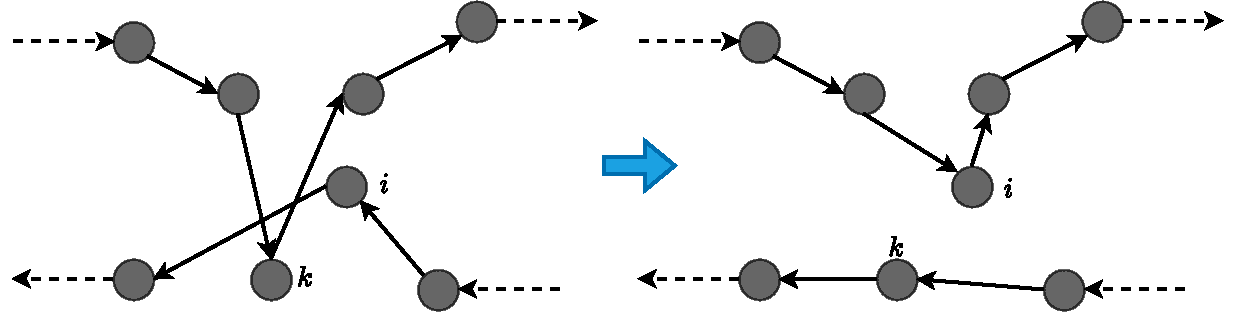
\includegraphics[width=0.8\textwidth]{images/exchange.pdf}
    \caption{exchange邻域结构}
    \label{fig:exchange邻域结构}
\end{figure}

第四种邻域结构为transfer方法,如图~\ref{fig:transfer邻域结构}所示。transfer方法是选取两任务点\( i \)和\( k \),将任务点\( i \)移出原任务序列,并将其插入至任务点\( k \)后,其余任务点及序列保持不变,以此来得到两条新的任务序列。

\begin{figure}[!htbp]
    \centering
    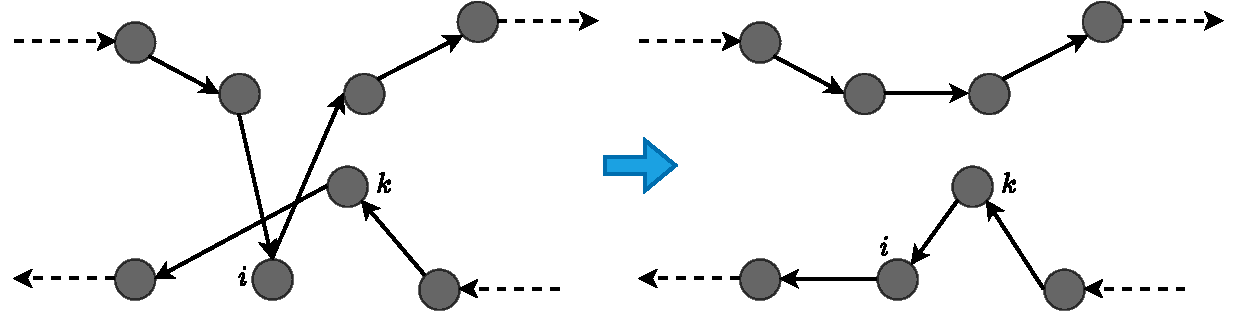
\includegraphics[width=0.8\textwidth]{images/transfer.pdf}
    \caption{transfer邻域结构}
    \label{fig:transfer邻域结构}
\end{figure}

第五种邻域结构为add new方法,如图~\ref{fig:add new邻域结构}所示。add new方法是选取一个任务点\( i \),将其从原任务序列中移除,其余任务点及序列保持不变,并将其作为新的无人机的任务序列,以此来得到两条新的任务序列。

\begin{figure}[!htbp]
    \centering
    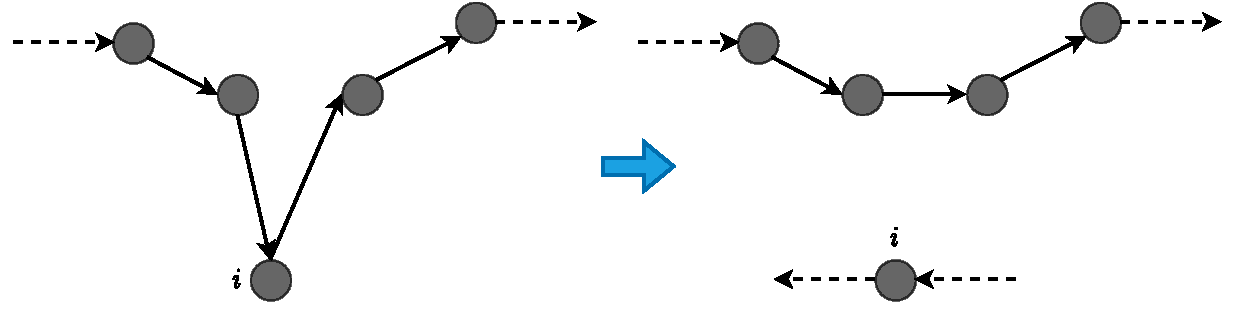
\includegraphics[width=0.8\textwidth]{images/add_new.pdf}
    \caption{add new邻域结构}
    \label{fig:add new邻域结构}
\end{figure}

由于模拟退火算法在运行中会存在初期温度高,同时未达到局部最优解的情况,以及末期温度低,同时达到局部最优解的情况,导致其非更优解接受概率的利用程度不高,所以模拟退火算法的性能仍有待提高。

为提高模拟退火算法的性能,更充分地利用其跳出局部最优解的机制,此处采用了自适应温度机制取代了原有的温度机制。

此处引入\(r_{i}\)作为算法第\(i\)次运行后没有得到更优解的次数,即需要计算非更优解接受概率的次数,当直接得到了更优解时\(r_{i} = 0\),算法未运行时\(r_{0} = 0\),即

\begin{equation}
    r_i = 
    \begin{aligned} 
    \begin{cases}
        r_{i-1} + 1 \quad &\text{if} \quad \Delta E > 0\\
        r_{i-1} &\text{if} \quad \Delta E = 0 \\
        0 &\text{if} \quad \Delta E <     0
    \end{cases}
    \end{aligned}
    \nonumber
\end{equation}

同时使用迭代次数\(N\)来控制整个算法的逻辑。与模拟退火算法相比,其总的求解次数仅由\(N\)决定,而模拟退火算法的总求解次数为\(N \cdot \log_{r}\frac{T_{0}}{T_{\text{end}}}\)。

设定一个最低温度\(T_{\min}\),升温速率\(\rho\)以及温控参数\(\delta\),使得第\(i\)次计算温度\(T_{i}\)时使用如下公式:

\begin{equation}
    T_i = T_{\min} + \rho \cdot \ln (1 + \frac{r_i}{\delta})
    \nonumber
\end{equation}

如此便能够在能够寻求到最优解的情况下维持低温,在到达局部最优解、需要到达新的局部最优解时能够通过升高温度来跳出局部最优解,从而使算法具有更好的鲁棒性。

\subsection{多无人机航迹规划及任务分配算法流程图}

由上述内容可知,本文提出的航迹规划及任务分配算法的流程如下,在任务开始前,服务器分别从贮存任务数据的数据库和地图信息的数据库中获取任务数据、地图数据,再将以上数据一齐输入进RRT*-Connect算法中,得到起飞点与任务点、任务点与任务点之间的无人机飞行航迹和飞行航程信息,将航程信息矩阵输入进K-Means算法中对任务进行预分配,再将任务的预分配结果、航程矩阵以及无人机的最大航程一齐输入进TSAVN算法中,便得到了完成任务所需的无人机数量以及每个无人机需完成的收集型侦察任务有序序列,再根据该序列从此前得到的点间飞行航迹中进行拼接得到各个无人机的飞行航迹,再将以上信息作为指令发送给无人机,由无人机完成所给任务。该算法的总流程如图~\ref{fig:航迹规划及任务分配流程图}所示。

\begin{figure}[!htbp]
    \centering
    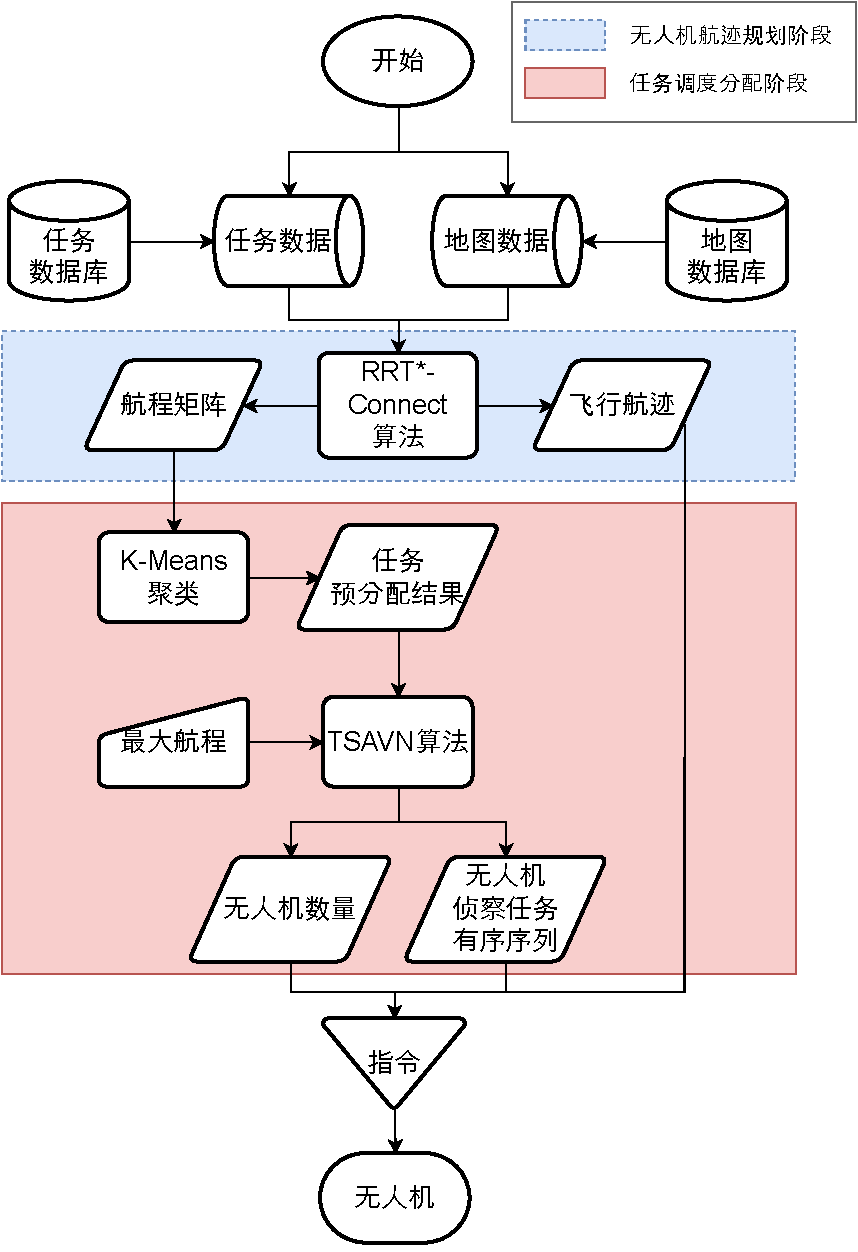
\includegraphics[width=0.7\textwidth]{images/任务分配及航迹规划算法流程图.drawio.pdf}
    \caption{航迹规划及任务分配流程图}
    \label{fig:航迹规划及任务分配流程图}
\end{figure}

\newpage
\section{本章小结}

本章主要对面向边缘计算的任务计算资源调度优化问题、多无人机的航迹规划及任务分配问题分别进行分析,并按照分析内容提出对应的求解算法,并详细说明了各个算法的关键机制、运行流程等内容。

\newpage


%!TEX root = ../../csuthesis_main.tex
\chapter{算法仿真实验}

\section{任务计算资源调度算法仿真实验}

为验证任务计算资源调度算法ASA和FD的有效性和优越性,本节完成并应用了任务生成器来随机生成包含着任务起始时间、所需计算资源、在不同设备上的计算时间、上传时延等的任务数据,并与采用了与ASA算法相同的邻域结构的SA算法进行测试对比。

\subsection{参数设置}

在设置任务生成器的参数时,本节使用了表~\ref{tab:资源分配算法任务生成参数}中的参数来生成近似真实应用场景下的计算型任务数据,其中任务总数\( N \)为50,每个任务的起始时间\(S_i\)为上下界分别为1000、0的离散型均匀分布,每个任务的计算所需资源\(R_i\)为上下界分别为100、1的离散型均匀分布,每个任务在无人机上计算需要花费的时间\(U_i\)为上下界300、1的离散性均匀分布,每个任务在服务器上计算需要花费的时间\(C_i\)为上下界\(U_i-1\)、0的离散性均匀分布,上传时延\(D_i\)为上下界100、1的离散型均匀分布。

\begin{table}[!htbp]
    \caption{资源分配算法任务生成参数}
    \label{tab:资源分配算法任务生成参数}
    \centering
    \begin{tabular}{c c c}
        \toprule
        \textbf{参数} & \textbf{含义} & \textbf{值}\\
        \midrule
        \( N \) & 任务总数 & 50 \\
        \( S_i \) & 第\(i\)个任务的起始时间 & \([0, 1000]\) \\
        \( R_i \) & 第\(i\)个任务所花费的资源 & \([1, 100]\) \\
        \( U_i \) & 第\(i\)个任务在无人机上计算需要花费的时间 & \([1, 300]\) \\
        \( C_i \) & 第\(i\)个任务在服务器上计算需要花费的时间 & \([0, U_i-1]\) \\
        \( D_i \) & 第\(i\)个任务上传至其他设备的时延 & \([1, 100]\) \\
        \bottomrule
    \end{tabular}
\end{table}

\begin{table}[!htbp]
    \caption{任务计算资源调度算法实验参数设置}
    \label{tab:任务计算资源调度算法实验参数设置}
    \centering
    \begin{tabular}{c c c}
        \toprule
        \textbf{参数} & \textbf{含义} & \textbf{值}\\
        \midrule
        \( N_u \) & 无人机数量 & 30 \\
        \( R_u \) & 无人机最大可用计算资源 & 100 \\
        \( N_c \) & 服务器数量 & 1 \\
        \( R_c \) & 服务器最大可用计算资源 & 2000 \\
        \bottomrule
    \end{tabular}
\end{table}


测试中采用的实验参数如表~\ref{tab:任务计算资源调度算法实验参数设置}所示,其中无人机的数量\( N_u \)为30,每架无人机最大可用的计算资源\(R_u\)为100,服务器的数量\( N_c \)为1,每台服务器最大可用的计算资源\( R_c \)为2000。

\begin{table}[!htbp]
    \caption{算法参数设置}
    \label{tab:算法参数设置}
    \centering
    \begin{tabular}{c c c c c c}
        \toprule
        \multicolumn{3}{c}{\textbf{SA}} & \multicolumn{3}{c}{\textbf{ASA}} \\
        \cmidrule(lr){1-3} \cmidrule(lr){4-6} 
        参数 & 含义 & 值 & 参数 & 含义 & 值\\
        \midrule
        \( T_{\textrm{init}} \) & 初始温度 & 1,000 & \( N \) & 总迭代次数 & 1000 \\
        \( T_{\textrm{end}} \) & 终止温度 & 1 & \( T_{\textrm{min}} \) & 最低温度 & 1 \\
        \( \rho_{\textrm{cool}} \) & 冷却速率 & 0.9 & \( \rho \) & 升温速率 & 1 \\
        \( n_T \) & 每个温度下的迭代次数 & 15 & \( \delta \) & 温控参数 & 0.01 \\
        \bottomrule
    \end{tabular}
\end{table}

本文所提出的ASA算法以及对比算法SA的参数设置如表~\ref{tab:算法参数设置}所示,即对于SA来说,其初始温度\( T_{\textrm{init}} \)为\(10^4\),终止温度\( T_{\textrm{end}} \)为\(10^{-1}\),冷却速率\( \rho_{\textrm{cool}} \)为0.9,每个温度下的迭代次数\(n_T\)为10,而对于ASA来说,其总迭代次数\(N\)为1000,最低温度\(T_{\textrm{min}}\)为1,升温速率\( \rho \)为1,温控参数\( \delta \)为1。

\subsection{算法性能对比实验结果}

为了能够直观地体现ASA算法的有效性及优越性,本节统计了十次性能测试的性能指标,其具体的性能结果如表~\ref{tab:资源分配算法性能比较结果}所示。

\begin{table}[!htbp]
    \caption{资源分配算法性能比较结果}
    \label{tab:资源分配算法性能比较结果}
    \centering
    \begin{tabular}{c c c c c c c}
        \toprule
        \multirow{2}{*}{\textbf{测试数据}} & \multicolumn{2}{c}{\textbf{SA}} & \multicolumn{2}{c}{\textbf{ASA}} & \multicolumn{2}{c}{\textbf{FD}}\\
        \cmidrule(lr){2-3} \cmidrule(lr){4-5} \cmidrule(lr){6-7}
        & \makecell{运行时间\\(秒)} & 目标值 & \makecell{运行时间\\(秒)} & 目标值 & \makecell{运行时间(秒)} & 目标值 \\
        \midrule
        1 & 203.324 & 30372 & 198.497 & 30313 & 0.038 & 30480\\
        2 & 223.149 & 29809 & 177.082 & 29809 & 0.039 & 29809\\
        3 & 216.077 & 31359 & 174.673 & 31359 & 0.039 & 31408\\
        4 & 234.679 & 31732 & 172.580 & 31686 & 0.041 & 32188\\
        5 & 227.150 & 31067 & 197.496 & 30597 & 0.040 & 31116\\
        6 & 238.868 & 30780 & 185.066 & 30888 & 0.041 & 31272\\
        7 & 209.149 & 31986 & 187.116 & 31309 & 0.042 & 31986\\
        8 & 252.184 & 32551 & 179.438 & 32467 & 0.041 & 32683\\
        9 & 221.427 & 29638 & 179.438 & 29152 & 0.039 & 29915\\
        10 & 195.529 & 30699 & 160.609 & 30606 & 0.040 & 30883\\
        \textbf{平均值} & 222.238 & 30956.4 & 184.156 & \textbf{30818.6} & \textbf{0.040} & 31174\\
        \bottomrule
    \end{tabular}
\end{table}

根据表~\ref{tab:资源分配算法性能比较结果}的试验结果,在目标值方面,本文所提出的ASA算法相较其他对比算法,得到的解质量更好,这体现了ASA算法在解决无人机任务执行开始前的任务计算资源调度静态问题时的有效性;在运行时间方面,ASA算法相较于SA算法有着更少的算法运行时间,同时FD算法的运行时间与其他算法的运行时间更是有着明显的差距,而FD算法虽然得到的解的质量较差,但由于其用于无人机任务执行开始后的动态问题,相较于目标性能,其运行时间更为重要。因此本文的ASA算法与FD算法在该问题下的优越性明显。

\section{静态场景下的无人机航迹规划算法仿真实验}

为验证本文所提出的静态场景下的无人机航迹规划算法RRT*-Connect的有效性及优越性,本节完成并应用了地图生成器来随机生成包含着不同障碍物、起终点的地图信息进行测试,并与其他同样能够用于航迹规划的Basic RRT算法、基于概率的RRT算法、RRT-Connect以及RRT*算法进行测试比较。

\subsection{仿真参数设置}

在设置地图生成器的参数时,本节使用了表~\ref{tab:航迹规划算法仿真环境参数}中的参数来生成近似真实城市环境的三维地图,其中该地图的大小为\( B_x \times B_y \times B_z \),每个位置的生成建筑物的概率\( P_b \)为10\%,建筑物的高度分布为均值\( \mu = B_z / 2\)的均值分布,建筑物所占地面面积\( S_b \)为固定为1,共生成\( N \)个测试地图。

\begin{table}[!htbp]
    \caption{静态场景下的无人机航迹规划算法仿真环境参数}
    \label{tab:航迹规划算法仿真环境参数}
    \centering
    \begin{tabular}{c c c}
        \toprule
        \textbf{参数} & \textbf{含义} & \textbf{值}\\
        \midrule
        \(B_x\) & 地图在\(x\)轴上的长度 & \(100\) \\
        \(B_y\) & 地图在\(y\)轴上的长度 & \(100\) \\
        \(B_z\) & 地图在\(z\)轴上的长度 & \(10\) \\
        \(P_b\) & 建筑物的生成概率 & \(10\%\)\\
        \( \mu \) & 建筑物高度的分布均值 & \(50\) \\
        \( S_b \) & 建筑物所占地面面积 & \(1\) \\
        \(N\) & 进行测试的地图数量 & \(100\) \\
        \bottomrule
    \end{tabular}
\end{table}

本文提出的RRT*-Connect算法与对比算法Basic RRT算法、基于概率的RRT算法、RRT-Connect算法与RRT*算法均采用相同的参数设置,即表~\ref{tab:无人机航迹规划算法参数设置}中所示,即对于上述每一个算法生成的随机树来说,其可容许的最大的步进拓展的长度\(S\)为1,在对地图进行采样时选取目标点的概率\(P_t\)为0.2。

\begin{table}[!htbp]
    \caption{静态场景下的无人机航迹规划算法参数设置}
    \label{tab:无人机航迹规划算法参数设置}
    \centering
    \begin{tabular}{c c c}
        \toprule
        \textbf{参数} & \textbf{含义} & \textbf{值}\\
        \midrule
        \( S \) & 步进长度 & 1\\
        \( P_t \) & 采样时选取目标点的概率 & 0.2\\
        \bottomrule
    \end{tabular}
\end{table}

\subsection{仿真实验结果}

为了直观地体现RRT*-Connect算法的有效性,本节选取了其中一次测试的结果并使其可视化,其建筑分布、飞行航迹等信息如图~\ref{fig:RRT*-Connect在三维地图下的仿真结果}所示,从图中可以明显看出,基于RRT*-Connect的航迹规划算法在模拟城市的三维环境下成功地躲避了环境中的建筑物,并成功地在较短航程下到达了目标点。

\begin{figure}[!htbp]
    \centering
    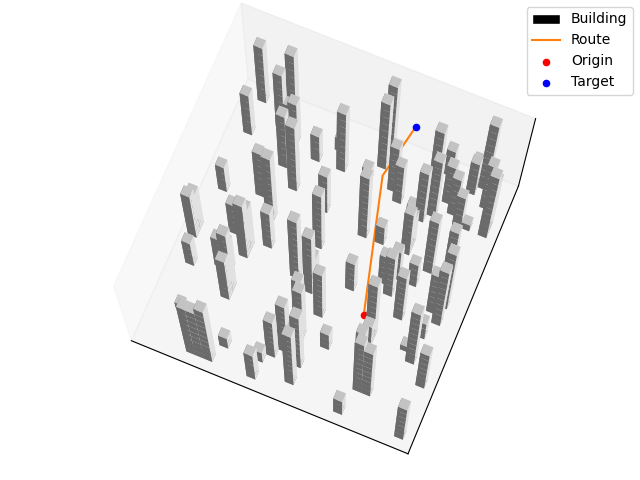
\includegraphics[width=0.75\textwidth]{./images/test_1_Connect_RRT_Star_1.png}
    \caption{基于RRT*-Connect的航迹规划算法在三维地图下的仿真结果}
    \label{fig:RRT*-Connect在三维地图下的仿真结果}
\end{figure}

\subsection{算法性能对比实验结果}

为了直观地体现RRT*-Connect算法的优越性,本节统计了性能测试中得到的性能指标,具体结果如表~\ref{tab:航迹规划算法性能比较结果}所示。

\begin{table}[!htbp]
    \caption{航迹规划算法性能比较结果}
    \label{tab:航迹规划算法性能比较结果}
    \centering
    \begin{tabular}{c c c}
        \toprule
        \textbf{算法} & \textbf{目标值} & \textbf{运行时间} \\
        \midrule
        Basic RRT & 105.313 & 4.008  \\
        基于概率的RRT & 87.878 & 3.710  \\
        RRT-Connect & 83.699 & \textbf{0.076} \\
        RRT* & 81.686 & 0.498 \\
        RRT*-Connect & \textbf{79.312} & 0.132 \\
        \bottomrule
    \end{tabular}:
\end{table}

根据表~\ref{tab:航迹规划算法性能比较结果}的试验结果,在目标值方面,本文所提出的RRT*-Connect算法相较其他对比算法,得到的解质量更好,这体现出了本文RRT*-Connect算法在解决城市密集障碍物环境下静态场景下的无人机航迹规划问题时的优越性;在运行时间方面,本文算法相较大部分对比算法而言有着更短的平均计算时间,仅相对于RRT-Connect在计算时间方面有着微小的差距,这是由于RRT*-Connect算法采用的Rewire机制导致算法计算量增加,进而造成计算时间的略微增加,但其求解结果却有了明显的提升。于此同时,由于本文研究的无人机航迹规划算法是在无人机任务执行开始之前,在服务器上运行生成航迹规划方案,相较于算法运行时间,其目标性能更为重要,因此本文的RRT*-Connect算法在该场景下的优越性更加明显。

\section{动态场景下的无人机航迹规划算法仿真实验}

为验证无人机实时避障算法A*的有效性及优越性,本节完成并应用了地图生成器来随机生成包含着不同障碍物、起终点的地图信息进行测试,并与同样能够应用于避障航迹生成的Basic RRT算法、基于概率的RRT算法、RRT-Connect、RRT*以及RRT*-Connect算法进行测试比较。

\subsection{仿真实验参数}

与静态场景下的航迹规划算法所解决的问题不同,动态场景下的无人机航迹规划算法所解决的动态场景下的无人机航迹规划问题的地图数据相对更小,且其实时性使得对算法的运行速度有着很高的要求,因此本文在设置地图生成器的参数时,为便于观察可视化结果,采用了表~\ref{tab:实时避障算法仿真环境参数}中的参数来随机生成包含不同障碍物、起终点的二维地图信息来生成算法的测试数据,其中,该地图大小为\( B_x \times B_y \),每个位置生成障碍物的概率\( P_b \)为\(10\%\),共生成\( N \)个测试地图。

\begin{table}[!htbp]
    \caption{动态场景下的无人机航迹规划算法仿真环境参数}
    \label{tab:实时避障算法仿真环境参数}
    \centering
    \begin{tabular}{c c c}
        \toprule
        \textbf{参数} & \textbf{含义} & \textbf{值}\\
        \midrule
        \(B_x\) & 地图在\(x\)轴上的长度 & \(30\) \\
        \(B_y\) & 地图在\(y\)轴上的长度 & \(30\) \\
        \(P_b\) & 障碍物的生成概率 & \(10\%\) \\
        \(N\) & 进行测试的地图数量 & \(100\) \\
        \bottomrule
    \end{tabular}
\end{table}

本文所使用的A*算法与对比算法Basic RRT算法、基于概率的RRT算法、RRT-Connect算法、RRT*算法与RRT*-Connect算法均采用相同的参数设置,即表~\ref{tab:实时避障算法参数设置}中所示,对于Basic RRT及其他基于Basic RRT的算法,采用RRT及其衍生算法下的参数,即其随机树的可容许最大步进拓展长度\(S\)为1,在对地图进行采样时选取目标点的概率\(P_t\)为0.2;对于A*算法而言,仅需设置其每一步的步进长度\(S\)为1。

\begin{table}[!htbp]
    \caption{动态场景下的无人机航迹规划算法参数设置}
    \label{tab:实时避障算法参数设置}
    \centering
    \begin{tabular}{c c c c c c}
        \toprule
        \multicolumn{3}{c}{\textbf{RRT及其衍生算法}} & \multicolumn{3}{c}{\textbf{A*}} \\
        \cmidrule(lr){1-3} \cmidrule(lr){4-6}
        参数 & 含义 & 值 & 参数 & 含义 & 值 \\
        \midrule
        \( S \) & 步进长度 & 1 & \( S \) & 步进长度 & 1 \\
        \( P_t \) & 采样时选取目标点的概率 & 0.2 & & & \\
        \bottomrule
    \end{tabular}
\end{table}

\subsection{仿真实验结果}

为了能够直观地体现A*的有效性,本节选取其中一次测试的结果并将其可视化,其障碍物分布、避障航迹如图~\ref{fig:A*算法在二维地图下的仿真结果}所示,从图中能够看出A*算法成功地根据已知障碍物信息规划出了一条能够躲避障碍物的飞行航迹。

\begin{figure}[!htbp]
    \centering
    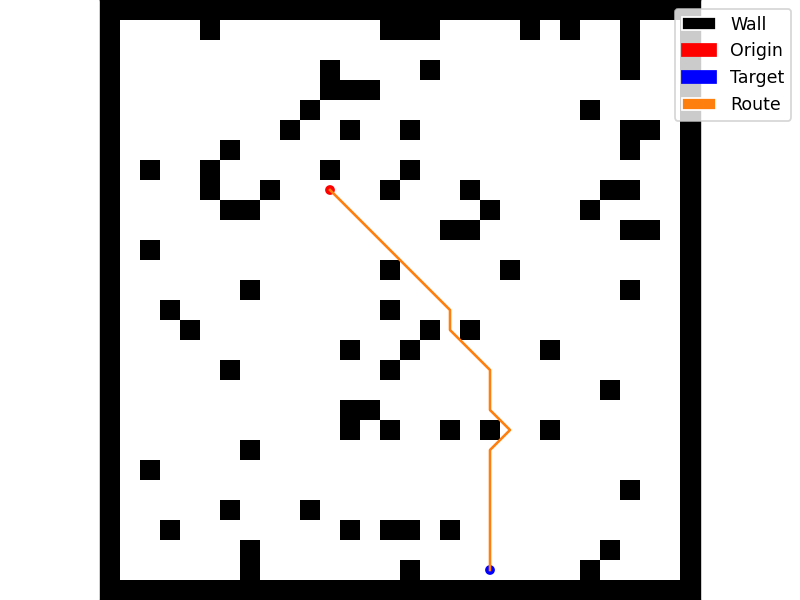
\includegraphics[width=0.65\textwidth]{images/test_8_A_Star.png}
    \caption{A*算法在二维地图下的仿真结果}
    \label{fig:A*算法在二维地图下的仿真结果}
\end{figure}

\subsection{算法性能对比实验结果}

为了直观地体现A*算法的优越性,本节统计了性能测试中得到的性能指标,具体的性能结果如表~\ref{tab:实时避障算法性能比较结果}所示,

\begin{longtable}{c c c}
    \caption{实时避障算法性能比较结果}
    \label{tab:实时避障算法性能比较结果}\\
        \toprule
        \textbf{算法} & \textbf{目标值} & \textbf{运行时间} \\
        \midrule
        Basic RRT & 29.459 & 0.070 \\
        基于概率的RRT & 24.876 & 0.077 \\
        RRT-Connect & 24.553 & 0.017 \\
        RRT* & 25.893 & 0.096 \\
        RRT*-Connect & 24.183 & 0.026 \\
        A* & \textbf{18.380} & \textbf{0.006} \\
        \bottomrule
\end{longtable}

根据表~\ref{tab:实时避障算法性能比较结果}的实验结果,在目标值方面,本文所使用的A*算法相较其他对比算法,得到的解质量更好,这体现了本文A*在解决城市密集障碍物环境下的动态场景下的无人机航迹规划问题的有效性;在运行时间方面,本文相较其他对比算法而言同样有着更少的平均计算时间。综上所述,本文的A*算法与其他算法相比具有显著的优越性。

\section{多无人机任务分配算法仿真实验}

为验证无人机任务分配算法TSAVN的有效性及优越性,考虑到无人机任务分配问题可以抽象为VRP问题,本节采用了\citet{gehring2002ParallelizationTwoPhaseMetaheuristic}的1000节点的硬时间窗VRP测试集中的\textit{c1\_10\_1}数据的前100个节点的位置信息作为测试数据,并加入了无人机最大航程的约束,并与同样能够用于无人机任务分配的基于RFCS(Routing First and Cluster Second,先规划后分配,在本问题中为先规划任务序列,再将该任务序列分配至无人机中)的遗传算法与模拟退火算法进行测试比较。

\subsection{实验参数设置}

本节采用的实验参数如表~\ref{tab:多无人机任务分配算法实验参数设置}所示,其中测试中采用的无人机飞行速度\(V_u\)为1,无人机最大航程\(\ell_{\textrm{max}}\)为3000,在目标函数中,无人机数量的惩罚系数\(P_u\)为1000。

\begin{table}[!htbp]
    \caption{多无人机任务分配算法实验参数设置}
    \label{tab:多无人机任务分配算法实验参数设置}
    \centering
    \begin{tabular}{c c c}
        \toprule
        \textbf{参数} & \textbf{含义} & \textbf{值} \\
        \midrule
        \( V_u \) & 无人机飞行速度 & 1 \\
        \( \ell_{\textrm{max}} \) & 无人机最大航程 & 3000 \\
        \( P_u \) & 无人机数量惩罚系数 & 1000\\
        \bottomrule
    \end{tabular}
\end{table}

本文所提出的TSAVN算法与对比算法GA、SA算法采用的参数设置如表~\ref{tab:无人机任务分配算法参数设置}中所示,即对于GA来说,其种群大小\(S_p\)为100,最大迭代次数\(N\)为1000,染色体的变异概率\(P_m\)为0.01,对于SA来说,其初始的温度\(T_{\textrm{init}}\)为100,最低温度\( T_{\textrm{min}} \)为\(10^{-7}\),马尔可夫链长度\( n_T \)为300,对于TSAVN来说,最大迭代次数\(N\)为1000,终止温度\( T_{\textrm{end}} \)为1升温速率\( \rho \)为1,温控参数\( \delta \)为1。

\begin{table}[!htbp]
    \caption{无人机任务分配算法参数设置}
    \label{tab:无人机任务分配算法参数设置}
    \centering
    \begin{tabular}{c c c c c c c c c}
        \toprule
        \multicolumn{3}{c}{\textbf{GA}} & \multicolumn{3}{c}{\textbf{SA}} & \multicolumn{3}{c}{\textbf{TSAVN}} \\
        \cmidrule(lr){1-3} \cmidrule(lr){4-6} \cmidrule(lr){7-9}
        参数 & 含义 & 值 & 参数 & 含义 & 值 & 参数 & 含义 & 值 \\
        \midrule
        \( S_p \) & 种群大小 & 100 & \( T_{\textrm{init}} \) & 初始温度 & 100 & \( N \) & 总迭代次数 & 1000\\
        \( N \) & 迭代次数 & 1000 & \( T_{\textrm{end}} \) & 终止温度 & \(10^{-7}\) & \( T_{\textrm{min}} \) & 最低温度 & 1\\
        \( P_m \) & 变异概率 & 0.01 & \( n_T \) & \makecell[c]{每个温度下的 \\ 迭代次数} & 300 &\( \rho \) & 升温速率 & 1\\
        & & & 冷却速率 & 0.9 & \( \rho \)  & \( \delta \) & 温控参数 & 1 \\
        \bottomrule
    \end{tabular}
\end{table}

\subsection{仿真实验结果}

为了直观地体现TSAVN算法的有效性,本节选取其中一次测试的结果并使其可视化,其所需无人机的数量、每个无人机的任务序列等信息如图~\ref{fig:基于TSAVN的多无人机算法仿真结果}所示,其中每一个叉为任务点的位置,每一种颜色的直线为每一个无人机的任务执行序列。各个无人机之间的规划路径不存在明显交叉情况,表明所提出的TSAVN算法在解决多无人机任务分配问题方面的有效性。

\begin{figure}[!htbp]
    \centering
    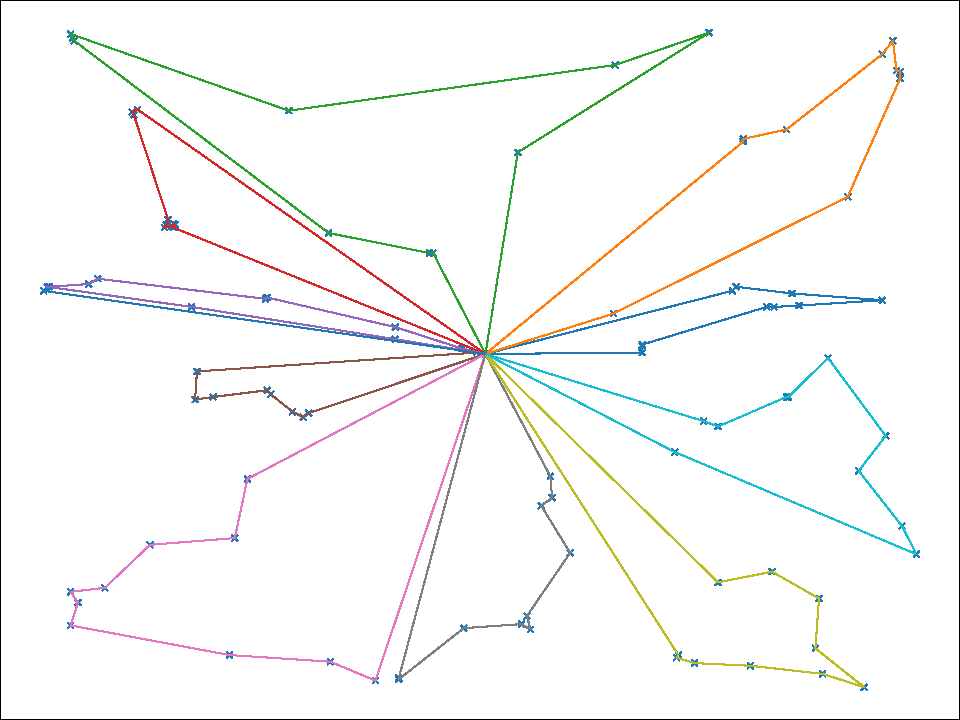
\includegraphics[width=0.45\textwidth]{images/TSAVN算法结果可视化.pdf}
    \caption{基于TSAVN的多无人机任务分配算法仿真结果}
    \label{fig:基于TSAVN的多无人机算法仿真结果}
\end{figure}

\subsection{算法性能对比实验结果}

为了直观地体现TSAVN算法的优越性,本节统计了性能测试中得到的性能指标,具体结果如表~\ref{tab:任务分配算法性能比较结果}所示。

\begin{table}[!htbp]
    \caption{任务分配算法性能比较结果}
    \label{tab:任务分配算法性能比较结果}
    \centering
    \begin{tabular}{c c c c c c c}
        \toprule
        \multirow{2}{*}{\textbf{运行次数}} & \multicolumn{2}{c}{\textbf{GA}} & \multicolumn{2}{c}{\textbf{SA}} & \multicolumn{2}{c}{\textbf{TSAVN}} \\
        \cmidrule(lr){2-3} \cmidrule(lr){4-5} \cmidrule(lr){6-7}
        & \makecell{运行时间\\(秒)} & 目标值 & \makecell{运行时间\\(秒)} & 目标值 & \makecell{运行时间\\(秒)} & 目标值 \\
        \midrule
        1 & 2086.7 & 66764.45 & 222.1 & 20759.26 & 9.731 & 18172.71\\
        2 & 1189.4 & 55713.22 & 204.2 & 19708.96 & 9.690 & 17882.67\\
        3 & 1181.4 & 52783.19 & 319.3 & 19358.90 & 9.155 & 17812.66\\
        4 & 1185.5 & 52623.57 & 127.6 & 20409.14 & 8.901 & 18052.71\\
        5 & 1182.3 & 55103.41 & 533.7 & 19009.00 & 8.200 & 17772.66\\
        6 & 1179.9 & 53380.95 & 541.9 & 18658.84 & 9.291 & 17962.69\\
        7 & 1177.1 & 55751.29 & 142.6 & 20059.25 & 9.759 & 17862.59\\
        8 & 1176.2 & 54941.32 & 205.4 & 19709.03 & 9.200 & 17772.56\\
        9 & 1179.6 & 53533.34 & 213.9 & 19708.96 & 9.119 & 18222.80\\
        10 & 1185.5 & 53222.29 & 167.2 & 20059.34 & 8.725 & 17542.58\\
        \textbf{平均值} & 1272.370 & 55381.703 & 267.790 & 19744.068 & \textbf{9.1771} & \textbf{17905.663} \\
        \bottomrule
    \end{tabular}
\end{table}

根据表~\ref{tab:任务分配算法性能比较结果}的试验结果,在目标值方面,本文所提出的TSAVN算法相较其他对比算法,得到的解质量更好,这体现了本文TSAVN在解决基于城市交通侦察场景下的无人机任务分配问题的有效性;在运行时间方面,本文算法相较其他对比算法而言同样有着更少的平均计算时间。综上所述,本文的TSAVN算法与其他算法相比具有显著的优越性。

\section{本章小结}

本章主要对本文所提出的任务计算资源的调度优化算法、多无人机航迹规划及任务分配算法在仿真环境下与不同的算法进行了性能测试,并进行了本文提出的算法与不同的算法在算法求解、运算时间等方面进行了性能的比较,进而得到本文所提出的算法的有效性及优越性。

\newpage


%!TEX root = ../../csuthesis_main.tex
\chapter{总结与展望}

\section{总结}

本文的主要研究成果如下:

\begin{enumerate}[leftmargin=2em]
    \item {对无人机航迹规划及任务调度问题进行了具体的描述与内容分析,在基于边缘计算架构将其分解为面向边缘计算的任务计算资源调度优化问题、多无人机的航迹规划及任务分配问题等两个子问题,基于合理假设为这两个子问题分别构建任务计算资源的调度优化模型、多无人机航迹规划及任务分配模型,为系统研究这两个问题提供了研究基础;}

    \item {针对任务计算资源的调度优化问题,考虑静态和动态两种不同的场景,设计了面向边缘计算的任务资源调度算法ASA、FD,在性能测试中,通过与SA算法的比较,表明ASA算法在任务完成时间、设备空闲时间等目标值上更优,并且与SA算法相比运行时间有所减少,而FD算法虽然得到的解的质量较差,但是其运行时间非常短,能够满足动态场景下的计算资源调度问题的实时性要求;}

    \item {针对多无人机的任务分配及轨迹规划问题,设计了基于RRT*-Connect的静态场景下的无人机航迹规划算法、基于A*的动态场景下的无人机航迹规划算法和基于TSAVN的多无人机任务调度分配算法。在算法性能测试方面,将其与多种算法进行对比,验证了所提算法在求解相应问题时的有效性和优越性。}
\end{enumerate}

\section{展望}

本文使用的多种算法虽然系统地解决了无人机航迹规划及任务调度问题的两个子问题,取得了较好的成功,但在研究过程中还存在着一些不足,
未来需要对本文的研究问题和所用算法进行进一步的优化,主要的展望如下:

\begin{enumerate}[leftmargin=2em]
    \item {无人机实时避障算法中,设置的位置障碍物为固定的,且无人机传感器能够检测到,但实际环境中可能存在着细小的障碍物,例如电线、未知无人机等物体,对于这些物体,由于其可能因为动态性或无法侦测性,可能导致无人机出现损毁等现象,因此有必要进一步研究无人机对于动态或细小的障碍物的动态场景下的航迹规划算法;}

    \item {在任务计算资源调度优化问题中,为简化问题,本文假设无人机与无人机、无人机与服务器的通信延迟、计算型任务在无人机和服务器上计算所需要的时间是可以通过例如神经网络、支持向量机等模型进行预测的,但并没有进行深入研究及实现,且该问题对任务计算资源调度优化问题中起着非常大的影响作用,因此有必要进一步研究无人机与无人机、无人机与服务器的通信延迟、计算型任务在无人机和服务器上计算所需要的时间的预测方法;}

    \item {本文将无人机航迹规划及任务调度问题分解为了两个子问题,但并未将两个子问题合并后进行求解,因此本文的研究成果离实际应用还有一定距离。}
\end{enumerate}

\newpage







% % 主文件有代码去掉页眉章节编号的“.”,但这会因为bug导致无编号章节显示一个错误编号,所以这里在无编号章节之前再次重定义sectionmark。
% \renewcommand{\sectionmark}[1]{\markright{#1}}


%%%%%%%%%%%%%%%%%%%%%%%%%%%%%%%%%%%%%%%%%%%%%%%%%%
% 致谢
%
% 存储在\content\acknowledgements.tex文件中
% 根据本科生院的要求,致谢应该在参考文献的前面,不编章号,而附录应该位于参考文献后。
%%%%%%%%%%%%%%%%%%%%%%%%%%%%%%%%%%%%%%%%%%%%%%%%%%
%!TEX root = ../csuthesis_main.tex
\begin{acknowledgements} 

\end{acknowledgements}


%%%%%%%%%%%%%%%%%%%%%%%%%%%%%%%%%%%%%%%%%%%%%%%%%%
% 参考文献
%
% 编译过程自动生成参考文献
% 根据学校要求文中引用的文献应依次编序,
% 其序号用方括号括起,如[5]、[6],置于右上角。
%%%%%%%%%%%%%%%%%%%%%%%%%%%%%%%%%%%%%%%%%%%%%%%%%%
% 由于参考文献不是chapter,这句把参考文献加入目录
% \addcontentsline{toc}{chapter}{参考文献} 
\phantomsection 
\addcontentsline{toc}{chapter}{参考文献} 
\printbibliography
\newpage


%%%%%%%%%%%%%%%%%%%%%%%%%%%%%%%%%%%%%%%%%%%%%%%%%%
% 附录部分
%
% 存储在\content\appendix.tex文件中
% 不宜收入正文中,又有价值的内容可编入毕业论文(设计)的附录中。
% 大号的设计图纸;篇幅较大的计算机程序(以研究软件程序
% 为主的毕业论文(设计)题目,其程序可作为正文的一部分);
% 过长的公式推演过程
%%%%%%%%%%%%%%%%%%%%%%%%%%%%%%%%%%%%%%%%%%%%%%%%%%
\appendix
%!TEX root = ../csuthesis_main.tex
% \begin{appendixs} % 无章节编号
% \chapter{附录代码}


% \end{appendixs}



%%%%%%%%%%%%%%%%%%%%%%%%%%%%%%%%%%%%%%%%%%%%%%%%%%
% 科研成果
%
% TODO: 硕士博士学位论文需添加
%%%%%%%%%%%%%%%%%%%%%%%%%%%%%%%%%%%%%%%%%%%%%%%%%%

\end{document}
